
% Default to the notebook output style

    


% Inherit from the specified cell style.




    
\documentclass[12pt]{article}


    
    \usepackage{graphicx} % Used to insert images
    \usepackage{adjustbox} % Used to constrain images to a maximum size 
    \usepackage{color} % Allow colors to be defined
    \usepackage{enumerate} % Needed for markdown enumerations to work
    \usepackage{geometry} % Used to adjust the document margins
    \usepackage{amsmath} % Equations
    \usepackage{amssymb} % Equations
    \usepackage{eurosym} % defines \euro
    \usepackage[mathletters]{ucs} % Extended unicode (utf-8) support
    \usepackage[utf8x]{inputenc} % Allow utf-8 characters in the tex document
    \usepackage{fancyvrb} % verbatim replacement that allows latex
    \usepackage{grffile} % extends the file name processing of package graphics 
 % to support a larger range 
    % The hyperref package gives us a pdf with properly built
    % internal navigation ('pdf bookmarks' for the table of contents,
    % internal cross-reference links, web links for URLs, etc.)
    \usepackage{hyperref}
    \usepackage{longtable} % longtable support required by pandoc >1.10
    \usepackage{booktabs}  % table support for pandoc > 1.12.2
    \usepackage{ulem} % ulem is needed to support strikethroughs (\sout)
    \usepackage{rotating}

\newcommand{\areps}{\textit{Ann.\ Rev.\ Earth Planet\ Sci.}, }
\newcommand{\bssa}{\textit{Bull.\ Seism.\ Soc.\ Am.}, }
\newcommand{\eos}{\textit{Eos Trans.\ AGU}, } 
\newcommand{\eps}{\textit{Earth~Planets~Space},}
\newcommand{\epsl}{\textit{Earth~Planet.\ Sci.\ Lett.}, }
\newcommand{\gca}{\textit{Geochim.\ Cosmochim.\ Acta}, }
\newcommand{\geo}{\textit{Geology}, }
\newcommand{\geop}{\textit{Geophysics}, }
\newcommand{\gji}{\textit{Geophys.\ J\ Int.}, }
\newcommand{\gjras}{\textit{Geophys.\ J.\ R.\ Astr.\ Soc.}, }
\newcommand{\grl}{\textit{Geophys.\ Res.\ Lett.}, }
\newcommand{\gsab}{\textit{Geol.\ Soc.\ Am.\ Bull.},}
\newcommand{\gs}{\textit{Geophys.\ Surv.}, }
\newcommand{\jgr}{\textit{J.\ Geophys.\ Res.}, }
\newcommand{\jpo}{\textit{J.\ Phys.\ Oceanogr.}, } 
\newcommand{\jseis}{\textit{J.~Seismology}, }
\newcommand{\mnras}{\textit{Mon.\ Not.\ R.\ Astr.\ Soc.}, } 
\newcommand{\pag}{\textit{Pure Appl.\ Geophys.},}
\newcommand{\pepi}{\textit{Phys.\ Earth Planet.\ Inter.}, }
\newcommand{\rg}{\textit{Rev.\ Geophys.}, }
\newcommand{\tecto}{\textit{Tectonophysics}, }
\newcommand{\srl}{\textit{Seis. Res. Lett.}, }
    
    \definecolor{orange}{cmyk}{0,0.4,0.8,0.2}
    \definecolor{darkorange}{rgb}{.71,0.21,0.01}
    \definecolor{darkgreen}{rgb}{.12,.54,.11}
    \definecolor{myteal}{rgb}{.26, .44, .56}
    \definecolor{gray}{gray}{0.45}
    \definecolor{lightgray}{gray}{.95}
    \definecolor{mediumgray}{gray}{.8}
    \definecolor{inputbackground}{rgb}{.95, .95, .85}
    \definecolor{outputbackground}{rgb}{.95, .95, .95}
    \definecolor{traceback}{rgb}{1, .95, .95}
    % ansi colors
    \definecolor{red}{rgb}{.6,0,0}
    \definecolor{green}{rgb}{0,.65,0}
    \definecolor{brown}{rgb}{0.6,0.6,0}
    \definecolor{blue}{rgb}{0,.145,.698}
    \definecolor{purple}{rgb}{.698,.145,.698}
    \definecolor{cyan}{rgb}{0,.698,.698}
    \definecolor{lightgray}{gray}{0.5}
    
    % bright ansi colors
    \definecolor{darkgray}{gray}{0.25}
    \definecolor{lightred}{rgb}{1.0,0.39,0.28}
    \definecolor{lightgreen}{rgb}{0.48,0.99,0.0}
    \definecolor{lightblue}{rgb}{0.53,0.81,0.92}
    \definecolor{lightpurple}{rgb}{0.87,0.63,0.87}
    \definecolor{lightcyan}{rgb}{0.5,1.0,0.83}
    
    % commands and environments needed by pandoc snippets
    % extracted from the output of `pandoc -s`
    \providecommand{\tightlist}{%
      \setlength{\itemsep}{0pt}\setlength{\parskip}{0pt}}
    \DefineVerbatimEnvironment{Highlighting}{Verbatim}{commandchars=\\\{\}}
    % Add ',fontsize=\small' for more characters per line
    \newenvironment{Shaded}{}{}
    \newcommand{\KeywordTok}[1]{\textcolor[rgb]{0.00,0.44,0.13}{\textbf{{#1}}}}
    \newcommand{\DataTypeTok}[1]{\textcolor[rgb]{0.56,0.13,0.00}{{#1}}}
    \newcommand{\DecValTok}[1]{\textcolor[rgb]{0.25,0.63,0.44}{{#1}}}
    \newcommand{\BaseNTok}[1]{\textcolor[rgb]{0.25,0.63,0.44}{{#1}}}
    \newcommand{\FloatTok}[1]{\textcolor[rgb]{0.25,0.63,0.44}{{#1}}}
    \newcommand{\CharTok}[1]{\textcolor[rgb]{0.25,0.44,0.63}{{#1}}}
    \newcommand{\StringTok}[1]{\textcolor[rgb]{0.25,0.44,0.63}{{#1}}}
    \newcommand{\CommentTok}[1]{\textcolor[rgb]{0.38,0.63,0.69}{\textit{{#1}}}}
    \newcommand{\OtherTok}[1]{\textcolor[rgb]{0.00,0.44,0.13}{{#1}}}
    \newcommand{\AlertTok}[1]{\textcolor[rgb]{1.00,0.00,0.00}{\textbf{{#1}}}}
    \newcommand{\FunctionTok}[1]{\textcolor[rgb]{0.02,0.16,0.49}{{#1}}}
    \newcommand{\RegionMarkerTok}[1]{{#1}}
    \newcommand{\ErrorTok}[1]{\textcolor[rgb]{1.00,0.00,0.00}{\textbf{{#1}}}}
    \newcommand{\NormalTok}[1]{{#1}}
    
    % Additional commands for more recent versions of Pandoc
    \newcommand{\ConstantTok}[1]{\textcolor[rgb]{0.53,0.00,0.00}{{#1}}}
    \newcommand{\SpecialCharTok}[1]{\textcolor[rgb]{0.25,0.44,0.63}{{#1}}}
    \newcommand{\VerbatimStringTok}[1]{\textcolor[rgb]{0.25,0.44,0.63}{{#1}}}
    \newcommand{\SpecialStringTok}[1]{\textcolor[rgb]{0.73,0.40,0.53}{{#1}}}
    \newcommand{\ImportTok}[1]{{#1}}
    \newcommand{\DocumentationTok}[1]{\textcolor[rgb]{0.73,0.13,0.13}{\textit{{#1}}}}
    \newcommand{\AnnotationTok}[1]{\textcolor[rgb]{0.38,0.63,0.69}{\textbf{\textit{{#1}}}}}
    \newcommand{\CommentVarTok}[1]{\textcolor[rgb]{0.38,0.63,0.69}{\textbf{\textit{{#1}}}}}
    \newcommand{\VariableTok}[1]{\textcolor[rgb]{0.10,0.09,0.49}{{#1}}}
    \newcommand{\ControlFlowTok}[1]{\textcolor[rgb]{0.00,0.44,0.13}{\textbf{{#1}}}}
    \newcommand{\OperatorTok}[1]{\textcolor[rgb]{0.40,0.40,0.40}{{#1}}}
    \newcommand{\BuiltInTok}[1]{{#1}}
    \newcommand{\ExtensionTok}[1]{{#1}}
    \newcommand{\PreprocessorTok}[1]{\textcolor[rgb]{0.74,0.48,0.00}{{#1}}}
    \newcommand{\AttributeTok}[1]{\textcolor[rgb]{0.49,0.56,0.16}{{#1}}}
    \newcommand{\InformationTok}[1]{\textcolor[rgb]{0.38,0.63,0.69}{\textbf{\textit{{#1}}}}}
    \newcommand{\WarningTok}[1]{\textcolor[rgb]{0.38,0.63,0.69}{\textbf{\textit{{#1}}}}}
    
    
    % Define a nice break command that doesn't care if a line doesn't already
    % exist.
    \def\br{\hspace*{\fill} \\* }
    % Math Jax compatability definitions
    \def\gt{>}
    \def\lt{<}
    % Document parameters
    \title{ An introduction to SeisTomoPy }
\author{S. Durand, R. Abreu \& C. Thomas}
\date{}


      % Pygments definitions
    
\makeatletter
\def\PY@reset{\let\PY@it=\relax \let\PY@bf=\relax%
    \let\PY@ul=\relax \let\PY@tc=\relax%
    \let\PY@bc=\relax \let\PY@ff=\relax}
\def\PY@tok#1{\csname PY@tok@#1\endcsname}
\def\PY@toks#1+{\ifx\relax#1\empty\else%
    \PY@tok{#1}\expandafter\PY@toks\fi}
\def\PY@do#1{\PY@bc{\PY@tc{\PY@ul{%
    \PY@it{\PY@bf{\PY@ff{#1}}}}}}}
\def\PY#1#2{\PY@reset\PY@toks#1+\relax+\PY@do{#2}}

\expandafter\def\csname PY@tok@gd\endcsname{\def\PY@tc##1{\textcolor[rgb]{0.63,0.00,0.00}{##1}}}
\expandafter\def\csname PY@tok@gu\endcsname{\let\PY@bf=\textbf\def\PY@tc##1{\textcolor[rgb]{0.50,0.00,0.50}{##1}}}
\expandafter\def\csname PY@tok@gt\endcsname{\def\PY@tc##1{\textcolor[rgb]{0.00,0.27,0.87}{##1}}}
\expandafter\def\csname PY@tok@gs\endcsname{\let\PY@bf=\textbf}
\expandafter\def\csname PY@tok@gr\endcsname{\def\PY@tc##1{\textcolor[rgb]{1.00,0.00,0.00}{##1}}}
\expandafter\def\csname PY@tok@cm\endcsname{\let\PY@it=\textit\def\PY@tc##1{\textcolor[rgb]{0.25,0.50,0.50}{##1}}}
\expandafter\def\csname PY@tok@vg\endcsname{\def\PY@tc##1{\textcolor[rgb]{0.10,0.09,0.49}{##1}}}
\expandafter\def\csname PY@tok@vi\endcsname{\def\PY@tc##1{\textcolor[rgb]{0.10,0.09,0.49}{##1}}}
\expandafter\def\csname PY@tok@mh\endcsname{\def\PY@tc##1{\textcolor[rgb]{0.40,0.40,0.40}{##1}}}
\expandafter\def\csname PY@tok@cs\endcsname{\let\PY@it=\textit\def\PY@tc##1{\textcolor[rgb]{0.25,0.50,0.50}{##1}}}
\expandafter\def\csname PY@tok@ge\endcsname{\let\PY@it=\textit}
\expandafter\def\csname PY@tok@vc\endcsname{\def\PY@tc##1{\textcolor[rgb]{0.10,0.09,0.49}{##1}}}
\expandafter\def\csname PY@tok@il\endcsname{\def\PY@tc##1{\textcolor[rgb]{0.40,0.40,0.40}{##1}}}
\expandafter\def\csname PY@tok@go\endcsname{\def\PY@tc##1{\textcolor[rgb]{0.53,0.53,0.53}{##1}}}
\expandafter\def\csname PY@tok@cp\endcsname{\def\PY@tc##1{\textcolor[rgb]{0.74,0.48,0.00}{##1}}}
\expandafter\def\csname PY@tok@gi\endcsname{\def\PY@tc##1{\textcolor[rgb]{0.00,0.63,0.00}{##1}}}
\expandafter\def\csname PY@tok@gh\endcsname{\let\PY@bf=\textbf\def\PY@tc##1{\textcolor[rgb]{0.00,0.00,0.50}{##1}}}
\expandafter\def\csname PY@tok@ni\endcsname{\let\PY@bf=\textbf\def\PY@tc##1{\textcolor[rgb]{0.60,0.60,0.60}{##1}}}
\expandafter\def\csname PY@tok@nl\endcsname{\def\PY@tc##1{\textcolor[rgb]{0.63,0.63,0.00}{##1}}}
\expandafter\def\csname PY@tok@nn\endcsname{\let\PY@bf=\textbf\def\PY@tc##1{\textcolor[rgb]{0.00,0.00,1.00}{##1}}}
\expandafter\def\csname PY@tok@no\endcsname{\def\PY@tc##1{\textcolor[rgb]{0.53,0.00,0.00}{##1}}}
\expandafter\def\csname PY@tok@na\endcsname{\def\PY@tc##1{\textcolor[rgb]{0.49,0.56,0.16}{##1}}}
\expandafter\def\csname PY@tok@nb\endcsname{\def\PY@tc##1{\textcolor[rgb]{0.00,0.50,0.00}{##1}}}
\expandafter\def\csname PY@tok@nc\endcsname{\let\PY@bf=\textbf\def\PY@tc##1{\textcolor[rgb]{0.00,0.00,1.00}{##1}}}
\expandafter\def\csname PY@tok@nd\endcsname{\def\PY@tc##1{\textcolor[rgb]{0.67,0.13,1.00}{##1}}}
\expandafter\def\csname PY@tok@ne\endcsname{\let\PY@bf=\textbf\def\PY@tc##1{\textcolor[rgb]{0.82,0.25,0.23}{##1}}}
\expandafter\def\csname PY@tok@nf\endcsname{\def\PY@tc##1{\textcolor[rgb]{0.00,0.00,1.00}{##1}}}
\expandafter\def\csname PY@tok@si\endcsname{\let\PY@bf=\textbf\def\PY@tc##1{\textcolor[rgb]{0.73,0.40,0.53}{##1}}}
\expandafter\def\csname PY@tok@s2\endcsname{\def\PY@tc##1{\textcolor[rgb]{0.73,0.13,0.13}{##1}}}
\expandafter\def\csname PY@tok@nt\endcsname{\let\PY@bf=\textbf\def\PY@tc##1{\textcolor[rgb]{0.00,0.50,0.00}{##1}}}
\expandafter\def\csname PY@tok@nv\endcsname{\def\PY@tc##1{\textcolor[rgb]{0.10,0.09,0.49}{##1}}}
\expandafter\def\csname PY@tok@s1\endcsname{\def\PY@tc##1{\textcolor[rgb]{0.73,0.13,0.13}{##1}}}
\expandafter\def\csname PY@tok@ch\endcsname{\let\PY@it=\textit\def\PY@tc##1{\textcolor[rgb]{0.25,0.50,0.50}{##1}}}
\expandafter\def\csname PY@tok@m\endcsname{\def\PY@tc##1{\textcolor[rgb]{0.40,0.40,0.40}{##1}}}
\expandafter\def\csname PY@tok@gp\endcsname{\let\PY@bf=\textbf\def\PY@tc##1{\textcolor[rgb]{0.00,0.00,0.50}{##1}}}
\expandafter\def\csname PY@tok@sh\endcsname{\def\PY@tc##1{\textcolor[rgb]{0.73,0.13,0.13}{##1}}}
\expandafter\def\csname PY@tok@ow\endcsname{\let\PY@bf=\textbf\def\PY@tc##1{\textcolor[rgb]{0.67,0.13,1.00}{##1}}}
\expandafter\def\csname PY@tok@sx\endcsname{\def\PY@tc##1{\textcolor[rgb]{0.00,0.50,0.00}{##1}}}
\expandafter\def\csname PY@tok@bp\endcsname{\def\PY@tc##1{\textcolor[rgb]{0.00,0.50,0.00}{##1}}}
\expandafter\def\csname PY@tok@c1\endcsname{\let\PY@it=\textit\def\PY@tc##1{\textcolor[rgb]{0.25,0.50,0.50}{##1}}}
\expandafter\def\csname PY@tok@o\endcsname{\def\PY@tc##1{\textcolor[rgb]{0.40,0.40,0.40}{##1}}}
\expandafter\def\csname PY@tok@kc\endcsname{\let\PY@bf=\textbf\def\PY@tc##1{\textcolor[rgb]{0.00,0.50,0.00}{##1}}}
\expandafter\def\csname PY@tok@c\endcsname{\let\PY@it=\textit\def\PY@tc##1{\textcolor[rgb]{0.25,0.50,0.50}{##1}}}
\expandafter\def\csname PY@tok@mf\endcsname{\def\PY@tc##1{\textcolor[rgb]{0.40,0.40,0.40}{##1}}}
\expandafter\def\csname PY@tok@err\endcsname{\def\PY@bc##1{\setlength{\fboxsep}{0pt}\fcolorbox[rgb]{1.00,0.00,0.00}{1,1,1}{\strut ##1}}}
\expandafter\def\csname PY@tok@mb\endcsname{\def\PY@tc##1{\textcolor[rgb]{0.40,0.40,0.40}{##1}}}
\expandafter\def\csname PY@tok@ss\endcsname{\def\PY@tc##1{\textcolor[rgb]{0.10,0.09,0.49}{##1}}}
\expandafter\def\csname PY@tok@sr\endcsname{\def\PY@tc##1{\textcolor[rgb]{0.73,0.40,0.53}{##1}}}
\expandafter\def\csname PY@tok@mo\endcsname{\def\PY@tc##1{\textcolor[rgb]{0.40,0.40,0.40}{##1}}}
\expandafter\def\csname PY@tok@kd\endcsname{\let\PY@bf=\textbf\def\PY@tc##1{\textcolor[rgb]{0.00,0.50,0.00}{##1}}}
\expandafter\def\csname PY@tok@mi\endcsname{\def\PY@tc##1{\textcolor[rgb]{0.40,0.40,0.40}{##1}}}
\expandafter\def\csname PY@tok@kn\endcsname{\let\PY@bf=\textbf\def\PY@tc##1{\textcolor[rgb]{0.00,0.50,0.00}{##1}}}
\expandafter\def\csname PY@tok@cpf\endcsname{\let\PY@it=\textit\def\PY@tc##1{\textcolor[rgb]{0.25,0.50,0.50}{##1}}}
\expandafter\def\csname PY@tok@kr\endcsname{\let\PY@bf=\textbf\def\PY@tc##1{\textcolor[rgb]{0.00,0.50,0.00}{##1}}}
\expandafter\def\csname PY@tok@s\endcsname{\def\PY@tc##1{\textcolor[rgb]{0.73,0.13,0.13}{##1}}}
\expandafter\def\csname PY@tok@kp\endcsname{\def\PY@tc##1{\textcolor[rgb]{0.00,0.50,0.00}{##1}}}
\expandafter\def\csname PY@tok@w\endcsname{\def\PY@tc##1{\textcolor[rgb]{0.73,0.73,0.73}{##1}}}
\expandafter\def\csname PY@tok@kt\endcsname{\def\PY@tc##1{\textcolor[rgb]{0.69,0.00,0.25}{##1}}}
\expandafter\def\csname PY@tok@sc\endcsname{\def\PY@tc##1{\textcolor[rgb]{0.73,0.13,0.13}{##1}}}
\expandafter\def\csname PY@tok@sb\endcsname{\def\PY@tc##1{\textcolor[rgb]{0.73,0.13,0.13}{##1}}}
\expandafter\def\csname PY@tok@k\endcsname{\let\PY@bf=\textbf\def\PY@tc##1{\textcolor[rgb]{0.00,0.50,0.00}{##1}}}
\expandafter\def\csname PY@tok@se\endcsname{\let\PY@bf=\textbf\def\PY@tc##1{\textcolor[rgb]{0.73,0.40,0.13}{##1}}}
\expandafter\def\csname PY@tok@sd\endcsname{\let\PY@it=\textit\def\PY@tc##1{\textcolor[rgb]{0.73,0.13,0.13}{##1}}}

\def\PYZbs{\char`\\}
\def\PYZus{\char`\_}
\def\PYZob{\char`\{}
\def\PYZcb{\char`\}}
\def\PYZca{\char`\^}
\def\PYZam{\char`\&}
\def\PYZlt{\char`\<}
\def\PYZgt{\char`\>}
\def\PYZsh{\char`\#}
\def\PYZpc{\char`\%}
\def\PYZdl{\char`\$}
\def\PYZhy{\char`\-}
\def\PYZdq{\char`\'}
\def\PYZdq{\char`\"}
\def\PYZti{\char`\~}
% for compatibility with earlier versions
\def\PYZat{@}
\def\PYZlb{[}
\def\PYZrb{]}
\makeatother

\usepackage{color}
\newcommand{\N}[1]{\textcolor{red}{#1}}
\newcommand{\D}[1]{\textcolor{blue}{\tiny #1}}
\newcommand{\C}[1]{\textcolor{green}{#1}}


\usepackage{hyperref} 
\usepackage[sort&compress,square,comma,authoryear]{natbib}

    % Exact colors from NB
    \definecolor{incolor}{rgb}{0.0, 0.0, 0.5}
    \definecolor{outcolor}{rgb}{0.545, 0.0, 0.0}
    
    % Prevent overflowing lines due to hard-to-break entities
    \sloppy 
    % Setup hyperref package
    \hypersetup{
      breaklinks=true,  % so long urls are correctly broken across lines
      colorlinks=true,
      urlcolor=blue,
      linkcolor=darkorange,
      citecolor=darkgreen,
      }
    % Slightly bigger margins than the latex defaults
    
    \geometry{verbose,tmargin=1in,bmargin=1in,lmargin=1in,rmargin=1in}
    
    \begin{document}
    
\vfill
\maketitle 
\begin{center}
 
\includegraphics[scale=0.8]{SeisTomoPy_notebook/figures/logo2.png}
\end{center}
\vfill



\newpage
\tableofcontents

\newpage
  
\section{What is SeisTomoPy}

SeisTomoPy is a Python tool that facilitates the use of a suite of tomographic models available to the public, with a single program. SeisTomoPy provides six tools that allow to visualize tomographic models, compare them and extract information for further scientific purposes. The tool comes with a graphical interface with intuitive buttons and simple parameters but the same information can also be gained by using the Python class that can be run routinely in Python scripts. SeisTomoPy is  suited for global and spherical tomographic models  and is provided with a default list of recent tomographic models. However, the user can also upload additional models if desired.

SeisTomoPy  includes several recent tomographic models that are available to the community. In Table \ref{summary} we summarize the characteristics of the different models included in the first version of SeisTomoPy. For detailed information on each model the reader is referred to the original publication. 

\begin{sidewaystable}
\caption{Summary of the characteristics of every tomographic model included in SeisTomoPy. Abbreviations in the table: SW - Surface waves, BW - body waves, NM - normal modes, T - period, Sph. Harm. - spherical harmonics, $V_s, V_p, V_{sh}, V_{sv}$ - shear velocity, compressional velocity, horizontal shear velocity, vertical shear velocity, $\nu_\alpha, \nu_\rho$ - scaling factors such that $d\ln(V_p)=\nu_\alpha d\ln(V_s)$ and $d\ln(\rho)=\nu_\rho d\ln(V_s)$.}
\label{summary}
\scalebox{0.6}{
\begin{tabular}{|c|c|c|c|c|c|c|c|c|c|}\hline
Model & Data & Inverted & Lateral & Radial   & Theory & Reference & Scaling & Crustal & Global\\
&&parameter & param. & param. & used & model & laws & model & or upper mantle \\
\hline
 & SW phase velocities  && Sph. Harm. up to & 21 cubic  & &  & $\nu_\alpha$ varies from & Corrected &\\\
 S40RTS & BW travel times &$V_s$&   degree 40  & spline functions &  Ray theory & PREM iso. & 2 (surf) to 3 (CMB) & CRUST2.0& Global\\
\tiny  \citep{ritsema11}&  NM splitting coefficients &&  & &  &  &$\nu_\rho = 0.3$ & \tiny \citep{bassin00}&\\
\hline
 &SW phase velocities &&Spherical&16 cubic&& & & &\\
S362WMANI+M& Long period BW waveforms & $V_{sh}$, $V_{sv}$ &splines&splines&Ray theory&STW105&$\nu_\alpha = 0.55$&Corrected& Global\\
\tiny \citep{moulik13}&BW travel times& &&discontinuous&&\tiny \citep{kustowski08}&$\nu_\rho = 0$&  CRUST2.0&\\
&NM splitting coefficients& &&across 650 km&&&&&\\
\hline
& SW wavforms (T $>$ 60 s) & &Spherical & 20 cubic & 3-D synthetics & their own &$\nu_\alpha = 0.5$ &Corrected&\\
SEMUCB-WM1 & BW waveforms  & $V_{sh}$, $V_{sv}$ & splines &  splines  & and NACT & model & $\nu_\rho = 0$&smoothed version& Global\\
 \tiny \citep{french14} &(T $ >$ 36 s and T $>$ 32 s) &  &  &   &&  \tiny \citep{french14} && CRUST2.0& \\
\hline
SGLOBE-rani &SW phase velocities&$V_{sh}$, $V_{sv}$ &Sph. Harm. up to & 20 cubic &Ray theory & PREM aniso.& $\nu_\alpha = 0.5$&Corrected&  Global\\
 \tiny \citep{chang15}&BW travel times&&degree 35 &splines&&&$\nu_\rho = 0.4$& CRUST2.0&\\
\hline
 & SW phase velocities  && Sph. Harm. up to & 21 cubic  &  & &  $\nu_\alpha = 0.55$& &\\
  SEISGLOB1& NM splitting and &$V_s$&   degree 20  & spline functions & Ray theory &  PREM iso. &$\nu_\rho = 0.2$ & Inverted& Global\\
 \tiny \citep{durand16}&  coupling coefficients && & &  &  &&& \\
\hline
 & SW phase velocities  && Sph. Harm. up to & 21 cubic  &  & & &Corrected&\\
SP12RTS & BW travel times &$V_s$, $V_p$&   degree 12  & spline functions & Ray theory &   PREM iso. & $\nu_\rho = 0.3$&CRUST2.0&  Global\\
  \tiny \citep{koelemeijer16}&  NM splitting coefficients &&  & &  &  & &&\\
\hline
 & SW phase velocities  && &  &&  && &\\
  SEISGLOB2& NM splitting coefficients &$V_s$&   Sph. Harm. up to   &  21 cubic & Ray theory   & PREM iso. & $\nu_\alpha = 0.55$ & Corrected& Global\\
\tiny \citep{durand17} &  NM splitting and &&degree 40   & spline functions  &  &  &$\nu_\rho = 0.2$ & CRUST2.0&\\
  &  coupling coefficients && & &  &  &&& \\
\hline
  3D2016-09S& SW phase velocities &$V_{sv}$, $V_{sh}$&   Correlation length 200 km down to 750~km  &  Correlation length & Path average   & PREM aniso. &  & Corrected 3SMAC & Upper mantle\\
\tiny \citep{debayle16} &  && increases to 800 km down to 1000~km  &  50~km &  &  & & \tiny \citep{nataf93}&\\
\hline
\end{tabular}}
\end{sidewaystable}

Associated to this first library of models, we provide six tools that will aid  extracting  information about each of these models:
\begin{itemize}
\item Cross section for generating cross sections and extracting values of $V_s$, $V_p$ and density as input for AxiSEM to generate synthetic seismograms,
\item Map for producing global tomographic maps at a given depth,
\item Spectrum for computing the amplitude spectrum at any depth,
\item Correlation for computing the correlation at any depth between the different models,
\item Path for plotting wave paths on the top of tomographic models,
\item Travel Time for computing travel times of body waves for the different tomographic models.
\end{itemize}

SeisTomoPy has been developed for saving the generated results from each of the functions in output files or figures that can be used for further scientific studies. 

It is also possible to upload a model if desired. A package is provided in order to create new model files. Our choice was to  develop models in spherical harmonics which:
\begin{itemize}
\item 1) enables to store the models quite efficiently, and avoids to deal with huge model files,
\item 2) is an efficient way to compute any section, map, spectrum, etc, in a reasonable amount of time.
\end{itemize}
This means that certain tomographic models are not suitable to be included in the tool, in particular those with irregular parametrization and regional models. 

\newpage

\section{Requirements}

SeisTomoPy is a Python software that can run on any version of Python from 2.6 to 3.6. However, we highly recommend to install Python 3.6, since Python 2.7 will be maintained until 1$^\textrm{rst}$ January 2020 only. You can download anaconda using this link:

\noindent \url{https://www.anaconda.com/download/#macos}
\\
\\
SeisTomoPy has a number of dependencies listed below.

\begin{itemize}
    \item gfortran : GNU Fortran (MacPorts gcc48 4.8.5\_0) 4.8.5
\item Python 2.7, 3.5, 3.6
\item iPython 5.3.0
\item matplotlib 2.0.2
\item  numpy 1.11.0
\item obspy 1.0.1
\item pyqt 5.6.0
\item scipy 0.17.0
\end{itemize}
For installing the Python dependencies, please run :\\
\verb?conda install -c conda-forge matplotlib numpy obspy pyqt scipy pyqtgraph basemap proj4?\\

\noindent If there is any problem with the compilation of fortran source files, we recommand to install fortran using:\\
\url{https://gcc.gnu.org/wiki/GFortranBinaries}

\section{Installation}

Clone the git repository and install in an editable fashion:\\

\verb?$ git clone https://github.com/stephaniedurand/SeisTomoPy.git?

\verb?$ cd SeisTomoPy?

\verb?$ pip install -v -e .?
\\
\\
\noindent   \textcolor{red}{\textbf{This will install the package on your computer and it will create a directory}} \verb?SeisTomoPy_files? \textcolor{red}{\textbf{in your home directory that should not be modified or removed for any reason, otherwise, the package won't work.}} \\
\\
  \textcolor{red}{\textbf{It is possible to uninstall SeisTomoPy from anywhere on your computer with the command}}

\verb?$ pip uninstall SeisTomoPy?

\section{Reported bugs}

There is currently some bugs with the installation of Basemap package with Python 3.6 or more. This is not related to SeisTomoPy and the solution seems to depend on the installation of conda the user has. Many people reported that an installation of 

\verb?$ conda install -c conda-forge  proj4?\\
works. But it may not be sufficient.

  \section{How to use SeisTomoPy class}\label{how-to-use-SeisTomoPy-class }\label{important-starting-notes} 

Launch iPython. The first thing to do is to import SeisTomoPy so that you will
be able to use the various SeisTomoPy functions. 

    \begin{Verbatim}[commandchars=\\\{\}]
\PY{k+kn}{import} \PY{n+nn}{SeisTomoPy} 
\end{Verbatim}

\subsection{Cross sections}\label{crosspy}

The user can generate cross sections through \(V_p\), \(V_s\) or \(\rho\)
variations anywhere on Earth in some default tomographic models provided with the tool using \verb?SeisTomoPy.cross_section_plot?. This
generates directly the plot of the cross section. However, the user
could also be interested in getting the values of the cross section and
then perform some further calculations. This can also be achieved
running \verb?SeisTomoPy.cross_section?. The latter function returns as
outputs the matrix containing the cross section ($Z$) as well as the angle
($th$) and radius vectors ($r$) that the user would need if he desires to
perform further calculations with this cross section.

Below is an example of how to get a cross section beneath Africa using
both class. Pink circles show hot spot locations, white circles denote earthquake
locations and green, red and yellow circles the starting, ending and
mid-point, respectively, along the profile.

    \begin{Verbatim}[commandchars=\\\{\},fontsize=\footnotesize]
\PY{c+c1}{\PYZsh{} Setting parameters}
\PY{c+c1}{\PYZsh{} Model to be plotted}
\PY{c+c1}{\PYZsh{} Choose between: }
\PY{c+c1}{\PYZsh{} SEISGLOB2, S40RTS, SEMUCBWM1, S362WMANIM, SEISGLOB1, SP12RTS, SGLOBE, 3D2016, MYMODEL}
\PY{n}{model} \PY{o}{=} \PY{l+s+s1}{\PYZdq{}}\PY{l+s+s1}{SEISGLOB2}\PY{l+s+s1}{\PYZdq{}}  
\PY{c+c1}{\PYZsh{} Parameter to be plotted}
\PY{c+c1}{\PYZsh{} Choose between: VS, VP, RHO}
\PY{n}{para} \PY{o}{=} \PY{l+s+s1}{\PYZdq{}}\PY{l+s+s1}{VS}\PY{l+s+s1}{\PYZdq{}}    
\PY{c+c1}{\PYZsh{} Latitude of the starting point of the cross section}
\PY{n}{elat} \PY{o}{=} \PY{o}{\PYZhy{}}\PY{l+m+mi}{60}    
\PY{c+c1}{\PYZsh{} Longitude of the starting point of the cross section}
\PY{n}{elon} \PY{o}{=} \PY{o}{\PYZhy{}}\PY{l+m+mi}{49}   
\PY{c+c1}{\PYZsh{} Latitude of the ending point of the cross section}
\PY{n}{slat} \PY{o}{=} \PY{l+m+mi}{60} 
\PY{c+c1}{\PYZsh{} Longitude of the ending point of the cross section}
\PY{n}{slon} \PY{o}{=} \PY{l+m+mi}{119}  
\PY{c+c1}{\PYZsh{} Depth of the cross section}
\PY{n}{depth} \PY{o}{=} \PY{l+m+mi}{2890}      
\PY{c+c1}{\PYZsh{} Spherical harmonic degrees to be used}
\PY{n}{NSmax} \PY{o}{=} \PY{l+m+mi}{40}     
\PY{c+c1}{\PYZsh{} Maximal velocity perturbations for the colorbar}
\PY{n}{Vmax} \PY{o}{=} \PY{l+m+mi}{2}     

\PY{c+c1}{\PYZsh{} Running cross\PYZus{}section\PYZus{}plot}
\PY{n}{SeisTomoPy}\PY{o}{.}\PY{n}{cross\PYZus{}section\PYZus{}plot}\PY{p}{(}\PY{n}{model}\PY{p}{,}\PY{n}{para}\PY{p}{,}\PY{n}{elat}\PY{p}{,}\PY{n}{elon}\PY{p}{,}\PY{n}{slat}\PY{p}{,}\PY{n}{slon}\PY{p}{,}\PY{n}{depth}\PY{p}{,}\PY{n}{NSmax}\PY{p}{,}\PY{n}{Vmax}\PY{p}{)}

\PY{c+c1}{\PYZsh{} Running cross\PYZus{}section}
\PY{n}{Z}\PY{p}{,} \PY{n}{th}\PY{p}{,} \PY{n}{r} \PY{o}{=} \PY{n}{SeisTomoPy}\PY{o}{.}\PY{n}{cross\PYZus{}section}\PY{p}{(}\PY{n}{model}\PY{p}{,}\PY{n}{para}\PY{p}{,}\PY{n}{elat}\PY{p}{,}\PY{n}{elon}\PY{p}{,}\PY{n}{slat}\PY{p}{,}\PY{n}{slon}\PY{p}{,}\PY{n}{depth}\PY{p}{,}\PY{n}{NSmax}\PY{p}{)}
\end{Verbatim}

    \begin{center}
    \adjustimage{max size={0.6\linewidth}{0.9\paperheight}}{SeisTomoPy_notebook/figures/crosspy_51.png}
    \end{center}
    

    \subsection{Maps}\label{mappy}

The user can create maps at a given depth for the whole globe using
\verb?SeisTomoPy.tomomap_plot?. This generates directly the plot of the map.
It is also possible to obtain the  values of the
map and then perform some further calculations using \verb?SeisTomoPy.tomomap?

Below is an example of how to obtain a map for the tomographic model
3D2016-S09 at 50 km depth using both class. Pink circles show hotspot
locations and gray lines the plate boundaries.

    \begin{Verbatim}[commandchars=\\\{\},fontsize=\footnotesize]
\PY{c+c1}{\PYZsh{} Setting parameters}
\PY{c+c1}{\PYZsh{} Model to be plotted}
\PY{n}{model} \PY{o}{=} \PY{l+s+s1}{\PYZdq{}}\PY{l+s+s1}{3D2016}\PY{l+s+s1}{\PYZdq{}}   
\PY{c+c1}{\PYZsh{} Parameter to be plotted}
\PY{n}{para} \PY{o}{=} \PY{l+s+s1}{\PYZdq{}}\PY{l+s+s1}{VS}\PY{l+s+s1}{\PYZdq{}}  
\PY{c+c1}{\PYZsh{} Depth of the map to be plotted}
\PY{n}{depth} \PY{o}{=} \PY{l+m+mi}{50}   
\PY{c+c1}{\PYZsh{} Spherical harmonic degrees to be used}
\PY{n}{NSmax} \PY{o}{=} \PY{l+m+mi}{60}    
\PY{c+c1}{\PYZsh{} Central longitude}
\PY{c+c1}{\PYZsh{} default value 140 degrees}
\PY{n}{lon0} \PY{o}{=} \PY{l+m+mi}{140}  
\PY{c+c1}{\PYZsh{} Maximal velocity perturbations for the colorbar}
\PY{n}{Vmax} \PY{o}{=} \PY{l+m+mi}{2}      

\PY{c+c1}{\PYZsh{} Running tomomap\PYZus{}plot}
\PY{n}{SeisTomoPy}\PY{o}{.}\PY{n}{tomomap\PYZus{}plot}\PY{p}{(}\PY{n}{model}\PY{p}{,}\PY{n}{para}\PY{p}{,}\PY{n}{depth}\PY{p}{,}\PY{n}{NSmax}\PY{p}{,}\PY{n}{Vmax}\PY{p}{,}\PY{n}{lon0}\PY{p}{)}

\PY{c+c1}{\PYZsh{} Changing the central longitude}
\PY{n}{lon0} \PY{o}{=} \PY{l+m+mi}{0}  
\PY{n}{SeisTomoPy}\PY{o}{.}\PY{n}{tomomap\PYZus{}plot}\PY{p}{(}\PY{n}{model}\PY{p}{,}\PY{n}{para}\PY{p}{,}\PY{n}{depth}\PY{p}{,}\PY{n}{NSmax}\PY{p}{,}\PY{n}{Vmax}\PY{p}{,}\PY{n}{lon0}\PY{p}{)}

\PY{c+c1}{\PYZsh{} Running tomomap}
\PY{n}{Z}\PY{p}{,} \PY{n}{lat}\PY{p}{,} \PY{n}{lon} \PY{o}{=} \PY{n}{SeisTomoPy}\PY{o}{.}\PY{n}{tomomap}\PY{p}{(}\PY{n}{model}\PY{p}{,}\PY{n}{para}\PY{p}{,}\PY{n}{depth}\PY{p}{,}\PY{n}{NSmax}\PY{p}{)}
\end{Verbatim}

    \begin{center}
    \adjustimage{max size={0.6\linewidth}{0.9\paperheight}}{SeisTomoPy_notebook/figures/mappy_521.png}
    \end{center}

    \begin{center}
    \adjustimage{max size={0.6\linewidth}{0.9\paperheight}}{SeisTomoPy_notebook/figures/mappy_522.png}
    \end{center}
It is possible to change \(NSmax\) to a value below 60 in order to filter the model.

    \begin{Verbatim}[commandchars=\\\{\},fontsize=\footnotesize]
\PY{c+c1}{\PYZsh{} Filtering the model}
\PY{n}{NSmax} \PY{o}{=} \PY{l+m+mi}{18}
\PY{n}{SeisTomoPy}\PY{o}{.}\PY{n}{tomomap\PYZus{}plot}\PY{p}{(}\PY{n}{model}\PY{p}{,}\PY{n}{para}\PY{p}{,}\PY{n}{depth}\PY{p}{,}\PY{n}{NSmax}\PY{p}{,}\PY{n}{Vmax}\PY{p}{)}
\end{Verbatim}

    \begin{center}
    \adjustimage{max size={0.6\linewidth}{0.9\paperheight}}{SeisTomoPy_notebook/figures/mappy_523.png}
    \end{center}
    
  \textcolor{red}{\textbf{These first tools can also be used with an uploaded tomographic model (see section 7 for details). The user would then refer to the new model by setting:}}

 \begin{Verbatim}[commandchars=\\\{\},fontsize=\footnotesize]
\PY{n}{model} \PY{o}{=} \PY{l+s+s1}{\PYZdq{}}\PY{l+s+s1}{MYMODEL}\PY{l+s+s1}{\PYZdq{}}   
\end{Verbatim}

    \subsection{Spectrum}\label{specpy}

The user can compute the amplitude spectrum, \(S(X,z,l)\), for a given
model at a given depth, \(z\), for a given parameter, \(X\), and for a
certain spherical harmonic degree, \(l\), using \verb?SeisTomoPy.spectrum? and
\verb?SeisTomoPy.spectrum_fromfile?. The first one computes the spectrum for
the models included by default in SeisTomoPy while the second one
enables the user to compute the spectrum in another model as
long as the correct input file is uploaded. Please refer to  section \ref{format} for details about these files.

The spectrum is defined by:
\begin{equation}
    S\left(X,z,l\right)= \sqrt{\frac{1}{4\pi}\sum_{m=-l}^{l} \left(\frac{\delta X}{X}(z)\right)_{lm} \, \left(\frac{\delta X}{X}(z)\right)_{lm}^\star },
\end{equation}
where the exponent ``\(^{\star}\)'' denotes the complex conjugate and
$\left(\frac{\delta X}{X}(z)\right)_{lm}$ the spherical harmonic
coefficients of the considered parameter \(X\) for a given tomographic
model at depth \(z\). \(X\) stands for \(V_s\), \(V_p\) or density.

Below is first an example of obtained spectrum for various models at 520 km
depth, for parameter \(V_s\) and up to spherical harmonic degree 40. We 
then show how to get the spectrum for another model not included in SeisTomoPy.

    \begin{Verbatim}[commandchars=\\\{\},fontsize=\footnotesize]
\PY{k}{print}\PY{p}{(}\PY{l+s+s1}{\PYZdq{}}\PY{l+s+s1}{!!!!!!!!!!!!!!!!!!!!!!!!!!!!!!!!!!!!!!!!!!!!!!!!!!!!!!!!!!!!!!!}\PY{l+s+s1}{\PYZdq{}}\PY{p}{)}
\PY{k}{print}\PY{p}{(}\PY{l+s+s1}{\PYZdq{}}\PY{l+s+s1}{ Example of spectrum computed in the default tomographic models }\PY{l+s+s1}{\PYZdq{}}\PY{p}{)}
\PY{k}{print}\PY{p}{(}\PY{l+s+s1}{\PYZdq{}}\PY{l+s+s1}{!!!!!!!!!!!!!!!!!!!!!!!!!!!!!!!!!!!!!!!!!!!!!!!!!!!!!!!!!!!!!!!}\PY{l+s+s1}{\PYZdq{}}\PY{p}{)}

\PY{c+c1}{\PYZsh{} Setting parameters}
\PY{c+c1}{\PYZsh{} Models to be used for computing the spectrum}
\PY{n}{model1} \PY{o}{=} \PY{l+s+s1}{\PYZdq{}}\PY{l+s+s1}{SEISGLOB2}\PY{l+s+s1}{\PYZdq{}}     
\PY{n}{model2} \PY{o}{=} \PY{l+s+s1}{\PYZdq{}}\PY{l+s+s1}{SGLOBE}\PY{l+s+s1}{\PYZdq{}}
\PY{n}{model3} \PY{o}{=} \PY{l+s+s1}{\PYZdq{}}\PY{l+s+s1}{S40RTS}\PY{l+s+s1}{\PYZdq{}}
\PY{n}{model4} \PY{o}{=} \PY{l+s+s1}{\PYZdq{}}\PY{l+s+s1}{SEMUCBWM1}\PY{l+s+s1}{\PYZdq{}}
\PY{n}{model5} \PY{o}{=} \PY{l+s+s1}{\PYZdq{}}\PY{l+s+s1}{S362WMANIM}\PY{l+s+s1}{\PYZdq{}}
\PY{c+c1}{\PYZsh{} Depth at which the spectrum is computed}
\PY{n}{depth} \PY{o}{=} \PY{l+m+mi}{520}    
\PY{c+c1}{\PYZsh{} Parameter used for computing the spectrum}
\PY{n}{para} \PY{o}{=} \PY{l+s+s1}{\PYZdq{}}\PY{l+s+s1}{VS}\PY{l+s+s1}{\PYZdq{}}     
\PY{c+c1}{\PYZsh{} Maximum spherical harmonic degree up to which the spectrum is computed}
\PY{n}{NSmax} \PY{o}{=} \PY{l+m+mi}{40}       

\PY{c+c1}{\PYZsh{} Running spectrum}
\PY{n}{sp1} \PY{o}{=} \PY{n}{SeisTomoPy}\PY{o}{.}\PY{n}{spectrum}\PY{p}{(}\PY{n}{model1}\PY{p}{,}\PY{n}{para}\PY{p}{,}\PY{n}{depth}\PY{p}{,}\PY{n}{NSmax}\PY{p}{)}
\PY{n}{sp2} \PY{o}{=} \PY{n}{SeisTomoPy}\PY{o}{.}\PY{n}{spectrum}\PY{p}{(}\PY{n}{model2}\PY{p}{,}\PY{n}{para}\PY{p}{,}\PY{n}{depth}\PY{p}{,}\PY{n}{NSmax}\PY{p}{)}
\PY{n}{sp3} \PY{o}{=} \PY{n}{SeisTomoPy}\PY{o}{.}\PY{n}{spectrum}\PY{p}{(}\PY{n}{model3}\PY{p}{,}\PY{n}{para}\PY{p}{,}\PY{n}{depth}\PY{p}{,}\PY{n}{NSmax}\PY{p}{)}
\PY{n}{sp4} \PY{o}{=} \PY{n}{SeisTomoPy}\PY{o}{.}\PY{n}{spectrum}\PY{p}{(}\PY{n}{model4}\PY{p}{,}\PY{n}{para}\PY{p}{,}\PY{n}{depth}\PY{p}{,}\PY{n}{NSmax}\PY{p}{)}
\PY{n}{sp5} \PY{o}{=} \PY{n}{SeisTomoPy}\PY{o}{.}\PY{n}{spectrum}\PY{p}{(}\PY{n}{model5}\PY{p}{,}\PY{n}{para}\PY{p}{,}\PY{n}{depth}\PY{p}{,}\PY{n}{NSmax}\PY{p}{)}

\PY{c+c1}{\PYZsh{} Plotting the results }
\PY{n}{plt}\PY{o}{.}\PY{n}{plot}\PY{p}{(}\PY{n}{sp1}\PY{p}{[}\PY{p}{:}\PY{p}{,}\PY{l+m+mi}{0}\PY{p}{]}\PY{p}{,} \PY{n}{sp1}\PY{p}{[}\PY{p}{:}\PY{p}{,}\PY{l+m+mi}{1}\PY{p}{]}\PY{o}{/}\PY{n}{np}\PY{o}{.}\PY{n}{amax}\PY{p}{(}\PY{n}{sp1}\PY{p}{[}\PY{p}{:}\PY{p}{,}\PY{l+m+mi}{1}\PY{p}{]}\PY{p}{)}\PY{p}{,} \PY{n}{linewidth}\PY{o}{=}\PY{l+m+mf}{1.0}\PY{p}{,}\PY{n}{color}\PY{o}{=}\PY{l+s+s2}{\PYZdq{}}\PY{l+s+s2}{red}\PY{l+s+s2}{\PYZdq{}}\PY{p}{, ...}
	\PY{n}{marker}\PY{o}{=}\PY{l+s+s2}{\PYZdq{}}\PY{l+s+s2}{d}\PY{l+s+s2}{\PYZdq{}}\PY{p}{,}\PY{n}{markeredgecolor}\PY{o}{=}\PY{l+s+s2}{\PYZdq{}}\PY{l+s+s2}{k}\PY{l+s+s2}{\PYZdq{}}\PY{p}{,} \PY{n}{label}\PY{o}{=}\PY{n}{model1}\PY{p}{)}
\PY{n}{plt}\PY{o}{.}\PY{n}{plot}\PY{p}{(}\PY{n}{sp2}\PY{p}{[}\PY{p}{:}\PY{p}{,}\PY{l+m+mi}{0}\PY{p}{]}\PY{p}{,} \PY{n}{sp2}\PY{p}{[}\PY{p}{:}\PY{p}{,}\PY{l+m+mi}{1}\PY{p}{]}\PY{o}{/}\PY{n}{np}\PY{o}{.}\PY{n}{amax}\PY{p}{(}\PY{n}{sp2}\PY{p}{[}\PY{p}{:}\PY{p}{,}\PY{l+m+mi}{1}\PY{p}{]}\PY{p}{)}\PY{p}{,} \PY{n}{linewidth}\PY{o}{=}\PY{l+m+mf}{1.0}\PY{p}{,}\PY{n}{color}\PY{o}{=}\PY{l+s+s2}{\PYZdq{}}\PY{l+s+s2}{k}\PY{l+s+s2}{\PYZdq{}}\PY{p}{, ...}
	\PY{n}{marker}\PY{o}{=}\PY{l+s+s2}{\PYZdq{}}\PY{l+s+s2}{d}\PY{l+s+s2}{\PYZdq{}}\PY{p}{,}\PY{n}{markeredgecolor}\PY{o}{=}\PY{l+s+s2}{\PYZdq{}}\PY{l+s+s2}{k}\PY{l+s+s2}{\PYZdq{}}\PY{p}{,} \PY{n}{label}\PY{o}{=}\PY{n}{model2}\PY{p}{)}
\PY{n}{plt}\PY{o}{.}\PY{n}{plot}\PY{p}{(}\PY{n}{sp3}\PY{p}{[}\PY{p}{:}\PY{p}{,}\PY{l+m+mi}{0}\PY{p}{]}\PY{p}{,} \PY{n}{sp3}\PY{p}{[}\PY{p}{:}\PY{p}{,}\PY{l+m+mi}{1}\PY{p}{]}\PY{o}{/}\PY{n}{np}\PY{o}{.}\PY{n}{amax}\PY{p}{(}\PY{n}{sp3}\PY{p}{[}\PY{p}{:}\PY{p}{,}\PY{l+m+mi}{1}\PY{p}{]}\PY{p}{)}\PY{p}{,} \PY{n}{linewidth}\PY{o}{=}\PY{l+m+mf}{1.0}\PY{p}{,}\PY{n}{color}\PY{o}{=}\PY{l+s+s2}{\PYZdq{}}\PY{l+s+s2}{blue}\PY{l+s+s2}{\PYZdq{}}\PY{p}{, ...}
	\PY{n}{marker}\PY{o}{=}\PY{l+s+s2}{\PYZdq{}}\PY{l+s+s2}{d}\PY{l+s+s2}{\PYZdq{}}\PY{p}{,}\PY{n}{markeredgecolor}\PY{o}{=}\PY{l+s+s2}{\PYZdq{}}\PY{l+s+s2}{k}\PY{l+s+s2}{\PYZdq{}}\PY{p}{,} \PY{n}{label}\PY{o}{=}\PY{n}{model3}\PY{p}{)}
\PY{n}{plt}\PY{o}{.}\PY{n}{plot}\PY{p}{(}\PY{n}{sp4}\PY{p}{[}\PY{p}{:}\PY{p}{,}\PY{l+m+mi}{0}\PY{p}{]}\PY{p}{,} \PY{n}{sp4}\PY{p}{[}\PY{p}{:}\PY{p}{,}\PY{l+m+mi}{1}\PY{p}{]}\PY{o}{/}\PY{n}{np}\PY{o}{.}\PY{n}{amax}\PY{p}{(}\PY{n}{sp4}\PY{p}{[}\PY{p}{:}\PY{p}{,}\PY{l+m+mi}{1}\PY{p}{]}\PY{p}{)}\PY{p}{,} \PY{n}{linewidth}\PY{o}{=}\PY{l+m+mf}{1.0}\PY{p}{,}\PY{n}{color}\PY{o}{=}\PY{l+s+s2}{\PYZdq{}}\PY{l+s+s2}{dodgerblue}\PY{l+s+s2}{\PYZdq{}}\PY{p}{,...}
	\PY{n}{marker}\PY{o}{=}\PY{l+s+s2}{\PYZdq{}}\PY{l+s+s2}{d}\PY{l+s+s2}{\PYZdq{}}\PY{p}{,}\PY{n}{markeredgecolor}\PY{o}{=}\PY{l+s+s2}{\PYZdq{}}\PY{l+s+s2}{k}\PY{l+s+s2}{\PYZdq{}}\PY{p}{,} \PY{n}{label}\PY{o}{=}\PY{n}{model4}\PY{p}{)}
\PY{n}{plt}\PY{o}{.}\PY{n}{plot}\PY{p}{(}\PY{n}{sp5}\PY{p}{[}\PY{p}{:}\PY{p}{,}\PY{l+m+mi}{0}\PY{p}{]}\PY{p}{,} \PY{n}{sp5}\PY{p}{[}\PY{p}{:}\PY{p}{,}\PY{l+m+mi}{1}\PY{p}{]}\PY{o}{/}\PY{n}{np}\PY{o}{.}\PY{n}{amax}\PY{p}{(}\PY{n}{sp5}\PY{p}{[}\PY{p}{:}\PY{p}{,}\PY{l+m+mi}{1}\PY{p}{]}\PY{p}{)}\PY{p}{,} \PY{n}{linewidth}\PY{o}{=}\PY{l+m+mf}{1.0}\PY{p}{,}\PY{n}{color}\PY{o}{=}\PY{l+s+s2}{\PYZdq{}}\PY{l+s+s2}{cyan}\PY{l+s+s2}{\PYZdq{}}\PY{p}{,...}
	\PY{n}{marker}\PY{o}{=}\PY{l+s+s2}{\PYZdq{}}\PY{l+s+s2}{d}\PY{l+s+s2}{\PYZdq{}}\PY{p}{,}\PY{n}{markeredgecolor}\PY{o}{=}\PY{l+s+s2}{\PYZdq{}}\PY{l+s+s2}{k}\PY{l+s+s2}{\PYZdq{}}\PY{p}{,} \PY{n}{label}\PY{o}{=}\PY{n}{model5}\PY{p}{)}
\PY{n}{plt}\PY{o}{.}\PY{n}{legend}\PY{p}{(}\PY{n}{bbox\PYZus{}to\PYZus{}anchor}\PY{o}{=}\PY{p}{(}\PY{l+m+mf}{1.45}\PY{p}{,} \PY{l+m+mi}{1}\PY{p}{)}\PY{p}{)}
\PY{n}{plt}\PY{o}{.}\PY{n}{xlabel}\PY{p}{(}\PY{l+s+s2}{\PYZdq{}}\PY{l+s+s2}{Harmonic degree l}\PY{l+s+s2}{\PYZdq{}}\PY{p}{)}
\PY{n}{plt}\PY{o}{.}\PY{n}{ylabel}\PY{p}{(}\PY{l+s+s2}{\PYZdq{}}\PY{l+s+s2}{Spectrum amplitude}\PY{l+s+s2}{\PYZdq{}}\PY{p}{)}
\PY{n}{plt}\PY{o}{.}\PY{n}{xlim}\PY{p}{(}\PY{p}{[}\PY{l+m+mf}{0.5}\PY{p}{,} \PY{n}{NSmax}\PY{o}{+}\PY{l+m+mf}{0.5}\PY{p}{]}\PY{p}{)}
\PY{n}{plt}\PY{o}{.}\PY{n}{grid}\PY{p}{(}\PY{n}{color}\PY{o}{=}\PY{l+s+s1}{\PYZdq{}}\PY{l+s+s1}{k}\PY{l+s+s1}{\PYZdq{}}\PY{p}{,} \PY{n}{linestyle}\PY{o}{=}\PY{l+s+s1}{\PYZdq{}}\PY{l+s+s1}{\PYZhy{}\PYZhy{}}\PY{l+s+s1}{\PYZdq{}}\PY{p}{,} \PY{n}{linewidth}\PY{o}{=}\PY{l+m+mf}{0.5}\PY{p}{)}
\PY{n}{plt}\PY{o}{.}\PY{n}{rcParams}\PY{o}{.}\PY{n}{update}\PY{p}{(}\PY{p}{\PYZob{}}\PY{l+s+s1}{\PYZdq{}}\PY{l+s+s1}{font.size}\PY{l+s+s1}{\PYZdq{}}\PY{p}{:} \PY{l+m+mi}{12}\PY{p}{\PYZcb{}}\PY{p}{)}
\PY{n}{plt}\PY{o}{.}\PY{n}{show}\PY{p}{(}\PY{p}{)}

\PY{k}{print}\PY{p}{(}\PY{l+s+s1}{\PYZdq{}}\PY{l+s+s1}{!!!!!!!!!!!!!!!!!!!!!!!!!!!!!!!!!!!!!!!!!!!!!!!!!!!!!!!!!!!!!!!}\PY{l+s+s1}{\PYZdq{}}\PY{p}{)}
\PY{k}{print}\PY{p}{(}\PY{l+s+s1}{\PYZdq{}}\PY{l+s+s1}{  Example of spectrum computed in another model}\PY{l+s+s1}{\PYZdq{}}\PY{p}{)}
\PY{k}{print}\PY{p}{(}\PY{l+s+s1}{\PYZdq{}}\PY{l+s+s1}{!!!!!!!!!!!!!!!!!!!!!!!!!!!!!!!!!!!!!!!!!!!!!!!!!!!!!!!!!!!!!!!}\PY{l+s+s1}{\PYZdq{}}\PY{p}{)}

\PY{c+c1}{\PYZsh{} Running spectrum\PYZus{}fromfile}
\PY{n}{filename} \PY{o}{=} \PY{l+s+s1}{\PYZdq{}}\PY{l+s+s1}{SeisTomoPy\PYZus{}notebook/files/input\PYZus{}file\PYZus{}spectrum.xyz}\PY{l+s+s1}{\PYZdq{}}
\PY{n}{sp\PYZus{}fromfile} \PY{o}{=} \PY{n}{SeisTomoPy}\PY{o}{.}\PY{n}{spectrum\PYZus{}fromfile}\PY{p}{(}\PY{n}{filename}\PY{p}{,}\PY{n}{NSmax}\PY{p}{)}

\PY{c+c1}{\PYZsh{} Plotting the results }
\PY{n}{plt}\PY{o}{.}\PY{n}{plot}\PY{p}{(}\PY{n}{sp\PYZus{}fromfile}\PY{p}{[}\PY{p}{:}\PY{p}{,}\PY{l+m+mi}{0}\PY{p}{]}\PY{p}{,} \PY{n}{sp\PYZus{}fromfile}\PY{p}{[}\PY{p}{:}\PY{p}{,}\PY{l+m+mi}{1}\PY{p}{]}\PY{o}{/}\PY{n}{np}\PY{o}{.}\PY{n}{amax}\PY{p}{(}\PY{n}{sp\PYZus{}fromfile}\PY{p}{[}\PY{p}{:}\PY{p}{,}\PY{l+m+mi}{1}\PY{p}{]}\PY{p}{)}\PY{p}{, ...}
	 \PY{n}{linewidth}\PY{o}{=}\PY{l+m+mf}{1.0}\PY{p}{,}\PY{n}{color}\PY{o}{=}\PY{l+s+s2}{\PYZdq{}}\PY{l+s+s2}{orange}\PY{l+s+s2}{\PYZdq{}}\PY{p}{,}\PY{n}{marker}\PY{o}{=}\PY{l+s+s2}{\PYZdq{}}\PY{l+s+s2}{d}\PY{l+s+s2}{\PYZdq{}}\PY{p}{,}\PY{n}{markeredgecolor}\PY{o}{=}\PY{l+s+s2}{\PYZdq{}}\PY{l+s+s2}{k}\PY{l+s+s2}{\PYZdq{}}\PY{p}{, ...}
	\PY{n}{label}\PY{o}{=}\PY{l+s+s1}{\PYZdq{}}\PY{l+s+s1}{Spectrum from a file}\PY{l+s+s1}{\PYZdq{}}\PY{p}{)}
\PY{n}{plt}\PY{o}{.}\PY{n}{legend}\PY{p}{(}\PY{n}{bbox\PYZus{}to\PYZus{}anchor}\PY{o}{=}\PY{p}{(}\PY{l+m+mf}{1.55}\PY{p}{,} \PY{l+m+mi}{1}\PY{p}{)}\PY{p}{)}
\PY{n}{plt}\PY{o}{.}\PY{n}{xlabel}\PY{p}{(}\PY{l+s+s2}{\PYZdq{}}\PY{l+s+s2}{Harmonic degree l}\PY{l+s+s2}{\PYZdq{}}\PY{p}{)}
\PY{n}{plt}\PY{o}{.}\PY{n}{ylabel}\PY{p}{(}\PY{l+s+s2}{\PYZdq{}}\PY{l+s+s2}{Spectrum amplitude}\PY{l+s+s2}{\PYZdq{}}\PY{p}{)}
\PY{n}{plt}\PY{o}{.}\PY{n}{xlim}\PY{p}{(}\PY{p}{[}\PY{l+m+mf}{0.5}\PY{p}{,} \PY{n}{NSmax}\PY{o}{+}\PY{l+m+mf}{0.5}\PY{p}{]}\PY{p}{)}
\PY{n}{plt}\PY{o}{.}\PY{n}{grid}\PY{p}{(}\PY{n}{color}\PY{o}{=}\PY{l+s+s1}{\PYZdq{}}\PY{l+s+s1}{k}\PY{l+s+s1}{\PYZdq{}}\PY{p}{,} \PY{n}{linestyle}\PY{o}{=}\PY{l+s+s1}{\PYZdq{}}\PY{l+s+s1}{\PYZhy{}\PYZhy{}}\PY{l+s+s1}{\PYZdq{}}\PY{p}{,}\PY{n}{linewidth}\PY{o}{=}\PY{l+m+mf}{0.5}\PY{p}{)}
\PY{n}{plt}\PY{o}{.}\PY{n}{rcParams}\PY{o}{.}\PY{n}{update}\PY{p}{(}\PY{p}{\PYZob{}}\PY{l+s+s1}{\PYZdq{}}\PY{l+s+s1}{font.size}\PY{l+s+s1}{\PYZdq{}}\PY{p}{:} \PY{l+m+mi}{12}\PY{p}{\PYZcb{}}\PY{p}{)}
\PY{n}{plt}\PY{o}{.}\PY{n}{show}\PY{p}{(}\PY{p}{)}
\end{Verbatim}

    \begin{Verbatim}[commandchars=\\\{\},fontsize=\footnotesize]
!!!!!!!!!!!!!!!!!!!!!!!!!!!!!!!!!!!!!!!!!!!!!!!!!!!!!!!!!!!!!!!
   Example of spectrum computed in the default tomographic models 
!!!!!!!!!!!!!!!!!!!!!!!!!!!!!!!!!!!!!!!!!!!!!!!!!!!!!!!!!!!!!!!
    \end{Verbatim}

    \begin{center}
    \adjustimage{max size={0.9\linewidth}{0.9\paperheight}}{SeisTomoPy_notebook/figures/specpy_531.png}
    \end{center}

    \begin{Verbatim}[commandchars=\\\{\},fontsize=\footnotesize]
!!!!!!!!!!!!!!!!!!!!!!!!!!!!!!!!!!!!!!!!!!!!!!!!!!!!!!!!!!!!!!!
    Example of spectrum computed in another model 
!!!!!!!!!!!!!!!!!!!!!!!!!!!!!!!!!!!!!!!!!!!!!!!!!!!!!!!!!!!!!!!
    \end{Verbatim}

    \begin{center}
    \adjustimage{max size={0.9\linewidth}{0.9\paperheight}}{SeisTomoPy_notebook/figures/specpy_532.png}
    \end{center}
It is possible to run the spectrum calculations routinely, at
various depths for instance. The example below can take some
time to run, it can be reduced by changing

\verb?$ depths = np.arange(100,2900,100)?

to

\verb?$ depths = np.arange(100,1100,100)?

\noindent  for instance.

    \begin{Verbatim}[commandchars=\\\{\},fontsize=\footnotesize]
 \PY{c+c1}{\PYZsh{} Setting parameters}
 \PY{c+c1}{\PYZsh{} Model to be used for computing the spectrum}
 \PY{n}{model} \PY{o}{=} \PY{l+s+s1}{\PYZdq{}}\PY{l+s+s1}{SEISGLOB2}\PY{l+s+s1}{\PYZdq{}}     
 \PY{c+c1}{\PYZsh{} Depth range at which the spectrum is computed}
 \PY{n}{depths} \PY{o}{=} \PY{n}{np}\PY{o}{.}\PY{n}{arange}\PY{p}{(}\PY{l+m+mi}{100}\PY{p}{,}\PY{l+m+mi}{2900}\PY{p}{,}\PY{l+m+mi}{100}\PY{p}{)}
 \PY{c+c1}{\PYZsh{} Parameter used for computing the spectrum}
 \PY{n}{para} \PY{o}{=} \PY{l+s+s1}{\PYZdq{}}\PY{l+s+s1}{VS}\PY{l+s+s1}{\PYZdq{}}     
 \PY{c+c1}{\PYZsh{} Maximum spherical harmonic degree up to which the spectrum is computed}
 \PY{n}{NSmax} \PY{o}{=} \PY{l+m+mi}{40}
 
 \PY{n}{deg} \PY{o}{=} \PY{n}{np}\PY{o}{.}\PY{n}{arange}\PY{p}{(}\PY{l+m+mi}{1}\PY{p}{,}\PY{l+m+mi}{41}\PY{p}{,}\PY{l+m+mi}{1}\PY{p}{)}
 \PY{n}{sp1} \PY{o}{=} \PY{n}{np}\PY{o}{.}\PY{n}{zeros}\PY{p}{(}\PY{p}{[}\PY{n+nb}{len}\PY{p}{(}\PY{n}{deg}\PY{p}{)}\PY{p}{,}\PY{n+nb}{len}\PY{p}{(}\PY{n}{depths}\PY{p}{)}\PY{p}{]}\PY{p}{)}
 
 \PY{c+c1}{\PYZsh{} Running spectrum routinely at various depths}
 \PY{k}{for} \PY{n}{i} \PY{o+ow}{in} \PY{n+nb}{range}\PY{p}{(}\PY{n+nb}{len}\PY{p}{(}\PY{n}{depths}\PY{p}{)}\PY{p}{)}\PY{p}{:}
     \PY{n}{sp11} \PY{o}{=} \PY{n}{SeisTomoPy}\PY{o}{.}\PY{n}{spectrum}\PY{p}{(}\PY{n}{model}\PY{p}{,}\PY{n}{para}\PY{p}{,}\PY{n}{depths}\PY{p}{[}\PY{n}{i}\PY{p}{]}\PY{p}{,}\PY{n}{NSmax}\PY{p}{)}
     \PY{k}{for} \PY{n}{k} \PY{o+ow}{in} \PY{n+nb}{range}\PY{p}{(}\PY{n+nb}{len}\PY{p}{(}\PY{n}{deg}\PY{p}{)}\PY{p}{)}\PY{p}{:}
 \PY{n}{sp1}\PY{p}{[}\PY{n}{k}\PY{p}{,}\PY{n}{i}\PY{p}{]}\PY{o}{=}\PY{n}{sp11}\PY{p}{[}\PY{n}{k}\PY{p}{,}\PY{l+m+mi}{1}\PY{p}{]}

 \PY{c+c1}{\PYZsh{} Plotting the result}
 \PY{n}{X}\PY{p}{,} \PY{n}{Y} \PY{o}{=} \PY{n}{np}\PY{o}{.}\PY{n}{meshgrid}\PY{p}{(}\PY{n}{deg}\PY{p}{,} \PY{n}{depths}\PY{p}{)}
 \PY{n}{plt}\PY{o}{.}\PY{n}{subplots\PYZus{}adjust}\PY{p}{(}\PY{n}{bottom}\PY{o}{=}\PY{l+m+mf}{0.2}\PY{p}{,} \PY{n}{right}\PY{o}{=}\PY{l+m+mf}{0.5}\PY{p}{,} \PY{n}{left}\PY{o}{=}\PY{l+m+mf}{0.2}\PY{p}{,} \PY{n}{top}\PY{o}{=}\PY{l+m+mf}{0.9}\PY{p}{)}
 \PY{n}{plt}\PY{o}{.}\PY{n}{pcolormesh}\PY{p}{(}\PY{n}{X}\PY{p}{,} \PY{n}{Y}\PY{p}{,} \PY{p}{(}\PY{n}{np}\PY{o}{.}\PY{n}{log10}\PY{p}{(}\PY{n}{np}\PY{o}{.}\PY{n}{transpose}\PY{p}{(}\PY{n}{sp1}\PY{p}{)}\PY{p}{)}\PY{p}{)}\PY{p}{, ...}
 \PY{n}{   shading}\PY{o}{=}\PY{l+s+s1}{\PYZdq{}}\PY{l+s+s1}{gouraud}\PY{l+s+s1}{\PYZdq{}}\PY{p}{,} \PY{n}{cmap}\PY{o}{=}\PY{l+s+s1}{\PYZdq{}}\PY{l+s+s1}{jet}\PY{l+s+s1}{\PYZdq{}}\PY{p}{,} \PY{n}{vmin}\PY{o}{=}\PY{o}{\PYZhy{}}\PY{l+m+mi}{2}\PY{p}{,} \PY{n}{vmax}\PY{o}{=}\PY{l+m+mi}{0}\PY{p}{)}
 \PY{n}{plt}\PY{o}{.}\PY{n}{gca}\PY{p}{(}\PY{p}{)}\PY{o}{.}\PY{n}{invert\PYZus{}yaxis}\PY{p}{(}\PY{p}{)}
 \PY{n}{plt}\PY{o}{.}\PY{n}{ylabel}\PY{p}{(}\PY{l+s+s1}{\PYZdq{}}\PY{l+s+s1}{Depth (km)}\PY{l+s+s1}{\PYZdq{}}\PY{p}{)}
 \PY{n}{plt}\PY{o}{.}\PY{n}{xlabel}\PY{p}{(}\PY{l+s+s1}{\PYZdq{}}\PY{l+s+s1}{Harmonic degree l}\PY{l+s+s1}{\PYZdq{}}\PY{p}{)}
 \PY{n}{plt}\PY{o}{.}\PY{n}{grid}\PY{p}{(}\PY{n}{color}\PY{o}{=}\PY{l+s+s1}{\PYZdq{}}\PY{l+s+s1}{k}\PY{l+s+s1}{\PYZdq{}}\PY{p}{,} \PY{n}{linestyle}\PY{o}{=}\PY{l+s+s1}{\PYZdq{}}\PY{l+s+s1}{\PYZhy{}\PYZhy{}}\PY{l+s+s1}{\PYZdq{}}\PY{p}{,} \PY{n}{linewidth}\PY{o}{=}\PY{l+m+mf}{0.5}\PY{p}{)}
 \PY{n}{plt}\PY{o}{.}\PY{n}{rcParams}\PY{o}{.}\PY{n}{update}\PY{p}{(}\PY{p}{\PYZob{}}\PY{l+s+s1}{\PYZdq{}}\PY{l+s+s1}{font.size}\PY{l+s+s1}{\PYZdq{}}\PY{p}{:} \PY{l+m+mi}{12}\PY{p}{\PYZcb{}}\PY{p}{)}
 \PY{n}{plt}\PY{o}{.}\PY{n}{title}\PY{p}{(}\PY{l+s+s1}{\PYZdq{}}\PY{l+s+s1}{SEISGLOB2}\PY{l+s+s1}{\PYZdq{}}\PY{p}{)}
 \PY{n}{plt}\PY{o}{.}\PY{n}{colorbar}\PY{p}{(}\PY{p}{)}
 \PY{n}{plt}\PY{o}{.}\PY{n}{show}\PY{p}{(}\PY{p}{)}
\end{Verbatim}

    \begin{center}
    \adjustimage{scale=0.9}{SeisTomoPy_notebook/figures/specpy_533.png}
    \end{center}

    \subsection{Correlations}\label{corrpy}

The user can compute the correlation between two tomographic models, (1)
and (2), using \verb?SeisTomoPy.correlation?, \verb?SeisTomoPy.correlation_fromfile?
and \verb?SeisTomoPy.correlation_fromfile2?. The first one computes the
correlation between two models chosen from the included ones by default
in SeisTomoPy, while the second and third ones enable the user to
compute the correlation between either any model with one of the default
ones or between any other models that the user wishes to use. In order to
use the two last functions the user thus must provide the required input
file. Please refer to  section \ref{format} for details about these files.

The correlation can be carried out for any parameter \(X_1\) of model
(1) and \(X_2\) of model (2) and for the same depth between the two
models (\(z_1=z_2\)) or it could be for different depths
(\(z_1 \neq z_2\)). Correlations are computed at a given spherical
harmonic degree, \(l\), following:
\begin{equation}
    C(X_1,z_1,X_2,z_2,l) = \frac{\displaystyle \sum_{m=-l}^l  \left(\frac{\delta X_1}{X_1}(z_1)\right)_{lm}  \left(\frac{\delta X_2}{X_2}(z_2)\right)^\star_{lm}}{\sqrt{\displaystyle \sum_{m=-l}^l  \left(\frac{\delta X_1}{X_1}(z_1)\right)_{lm}  \left(\frac{\delta X_1}{X_1}(z_1)\right)^\star_{lm} \, \displaystyle \sum_{m=-l}^l  \left(\frac{\delta X_2}{X_2}(z_2)\right)_{lm}  \left(\frac{\delta X_2}{X_2}(z_2)\right)^\star_{lm}}}.
    \label{eq.Correlation}
\end{equation}

Below is an example of the correlation computed between SEISGLOB2 and S40RTS
 at 520 km depth, for parameter \(V_s\) and up to spherical
harmonic degree 40. We then  show how to find the correlation for any model not
included in SeisTomoPy.

    \begin{Verbatim}[commandchars=\\\{\},fontsize=\footnotesize]
\PY{k}{print}\PY{p}{(}\PY{l+s+s1}{\PYZdq{}}\PY{l+s+s1}{!!!!!!!!!!!!!!!!!!!!!!!!!!!!!!!!!!!!!!!!!!!!!!!!!!!!!!!!!!!!!!!!!!!!!!}\PY{l+s+s1}{\PYZdq{}}\PY{p}{)}
\PY{k}{print}\PY{p}{(}\PY{l+s+s1}{\PYZdq{}}\PY{l+s+s1}{Example of correlation computed betwenn the default tomographic models}\PY{l+s+s1}{\PYZdq{}}\PY{p}{)}
\PY{k}{print}\PY{p}{(}\PY{l+s+s1}{\PYZdq{}}\PY{l+s+s1}{!!!!!!!!!!!!!!!!!!!!!!!!!!!!!!!!!!!!!!!!!!!!!!!!!!!!!!!!!!!!!!!!!!!!!!}\PY{l+s+s1}{\PYZdq{}}\PY{p}{)}

\PY{c+c1}{\PYZsh{} Setting parameters}
\PY{c+c1}{\PYZsh{} Models to be used for computing the correlation}
\PY{n}{model1} \PY{o}{=} \PY{l+s+s1}{\PYZdq{}}\PY{l+s+s1}{SEISGLOB2}\PY{l+s+s1}{\PYZdq{}} 
\PY{n}{model2} \PY{o}{=} \PY{l+s+s1}{\PYZdq{}}\PY{l+s+s1}{S40RTS}\PY{l+s+s1}{\PYZdq{}}
\PY{c+c1}{\PYZsh{} Depth at which the correlation is computed}
\PY{n}{depth} \PY{o}{=} \PY{l+m+mi}{520}
\PY{c+c1}{\PYZsh{} Parameters used for computing the correlation}
\PY{n}{para1} \PY{o}{=} \PY{l+s+s1}{\PYZdq{}}\PY{l+s+s1}{VS}\PY{l+s+s1}{\PYZdq{}} 
\PY{n}{para2} \PY{o}{=} \PY{l+s+s1}{\PYZdq{}}\PY{l+s+s1}{VS}\PY{l+s+s1}{\PYZdq{}} 
\PY{c+c1}{\PYZsh{} Maximum spherical harmonic degree up to which the correlation is computed}
\PY{n}{NSmax} \PY{o}{=} \PY{l+m+mi}{40}

\PY{c+c1}{\PYZsh{} Running correlation}
\PY{n}{corr} \PY{o}{=} \PY{n}{SeisTomoPy}\PY{o}{.}\PY{n}{correlation}\PY{p}{(}\PY{n}{model1}\PY{p}{,}\PY{n}{model2}\PY{p}{,}\PY{n}{depth}\PY{p}{,}\PY{n}{depth}\PY{p}{,}\PY{n}{para1}\PY{p}{,}\PY{n}{para2}\PY{p}{,}\PY{n}{NSmax}\PY{p}{)}

\PY{n}{plt}\PY{o}{.}\PY{n}{plot}\PY{p}{(}\PY{n}{corr}\PY{p}{[}\PY{p}{:}\PY{p}{,}\PY{l+m+mi}{0}\PY{p}{]}\PY{p}{,}\PY{n}{corr}\PY{p}{[}\PY{p}{:}\PY{p}{,}\PY{l+m+mi}{1}\PY{p}{]}\PY{p}{,}\PY{n}{linewidth}\PY{o}{=}\PY{l+m+mf}{1.0}\PY{p}{,}\PY{n}{color}\PY{o}{=}\PY{l+s+s2}{\PYZdq{}}\PY{l+s+s2}{grey}\PY{l+s+s2}{\PYZdq{}}\PY{p}{,}\PY{n}{marker}\PY{o}{=}\PY{l+s+s2}{\PYZdq{}}\PY{l+s+s2}{d}\PY{l+s+s2}{\PYZdq{}}\PY{p}{, ...}
	\PY{n}{label}\PY{o}{=}\PY{n}{model1} \PY{o}{+} \PY{l+s+s1}{\PYZdq{}}\PY{l+s+s1}{\PYZhy{}}\PY{l+s+s1}{\PYZdq{}} \PY{o}{+} \PY{n}{model2}\PY{p}{)}
\PY{n}{conf66} \PY{o}{=} \PY{n}{np}\PY{o}{.}\PY{n}{loadtxt}\PY{p}{(}\PY{l+s+s1}{\PYZdq{}}\PY{l+s+s1}{conf66.dat}\PY{l+s+s1}{\PYZdq{}}\PY{p}{)}
\PY{n}{conf90} \PY{o}{=} \PY{n}{np}\PY{o}{.}\PY{n}{loadtxt}\PY{p}{(}\PY{l+s+s1}{\PYZdq{}}\PY{l+s+s1}{conf90.dat}\PY{l+s+s1}{\PYZdq{}}\PY{p}{)}
\PY{n}{conf95} \PY{o}{=} \PY{n}{np}\PY{o}{.}\PY{n}{loadtxt}\PY{p}{(}\PY{l+s+s1}{\PYZdq{}}\PY{l+s+s1}{conf95.dat}\PY{l+s+s1}{\PYZdq{}}\PY{p}{)}
\PY{n}{plt}\PY{o}{.}\PY{n}{plot}\PY{p}{(}\PY{n}{conf66}\PY{p}{[}\PY{p}{:}\PY{p}{,}\PY{l+m+mi}{0}\PY{p}{]}\PY{p}{,} \PY{n}{conf66}\PY{p}{[}\PY{p}{:}\PY{p}{,}\PY{l+m+mi}{1}\PY{p}{]}\PY{p}{,} \PY{n}{linewidth}\PY{o}{=}\PY{l+m+mf}{1.0}\PY{p}{,}\PY{n}{color}\PY{o}{=}\PY{l+s+s2}{\PYZdq{}}\PY{l+s+s2}{silver}\PY{l+s+s2}{\PYZdq{}}\PY{p}{,} \PY{n}{ls}\PY{o}{=}\PY{l+s+s1}{\PYZdq{}}\PY{l+s+s1}{\PYZhy{}\PYZhy{}}\PY{l+s+s1}{\PYZdq{}}\PY{p}{, ...}
	\PY{n}{label}\PY{o}{=}\PY{l+s+s1}{\PYZdq{}}\PY{l+s+s1}{Confidence level 66}\PY{l+s+s1}{\PYZpc{}}\PY{l+s+s1}{\PYZdq{}}\PY{p}{)}
\PY{n}{plt}\PY{o}{.}\PY{n}{plot}\PY{p}{(}\PY{n}{conf90}\PY{p}{[}\PY{p}{:}\PY{p}{,}\PY{l+m+mi}{0}\PY{p}{]}\PY{p}{,} \PY{n}{conf90}\PY{p}{[}\PY{p}{:}\PY{p}{,}\PY{l+m+mi}{1}\PY{p}{]}\PY{p}{,} \PY{n}{linewidth}\PY{o}{=}\PY{l+m+mf}{1.0}\PY{p}{,}\PY{n}{color}\PY{o}{=}\PY{l+s+s2}{\PYZdq{}}\PY{l+s+s2}{gray}\PY{l+s+s2}{\PYZdq{}}\PY{p}{,} \PY{n}{ls}\PY{o}{=}\PY{l+s+s1}{\PYZdq{}}\PY{l+s+s1}{\PYZhy{}\PYZhy{}}\PY{l+s+s1}{\PYZdq{}}\PY{p}{, ...}
\PY{n}{label}\PY{o}{=}\PY{l+s+s1}{\PYZdq{}}\PY{l+s+s1}{Confidence level 90}\PY{l+s+s1}{\PYZpc{}}\PY{l+s+s1}{\PYZdq{}}\PY{p}{)}
\PY{n}{plt}\PY{o}{.}\PY{n}{plot}\PY{p}{(}\PY{n}{conf95}\PY{p}{[}\PY{p}{:}\PY{p}{,}\PY{l+m+mi}{0}\PY{p}{]}\PY{p}{,} \PY{n}{conf95}\PY{p}{[}\PY{p}{:}\PY{p}{,}\PY{l+m+mi}{1}\PY{p}{]}\PY{p}{,} \PY{n}{linewidth}\PY{o}{=}\PY{l+m+mf}{1.0}\PY{p}{,}\PY{n}{color}\PY{o}{=}\PY{l+s+s2}{\PYZdq{}}\PY{l+s+s2}{black}\PY{l+s+s2}{\PYZdq{}}\PY{p}{,} \PY{n}{ls}\PY{o}{=}\PY{l+s+s1}{\PYZdq{}}\PY{l+s+s1}{\PYZhy{}\PYZhy{}}\PY{l+s+s1}{\PYZdq{}}\PY{p}{, ...}
	\PY{n}{label}\PY{o}{=}\PY{l+s+s1}{\PYZdq{}}\PY{l+s+s1}{Confidence level 95}\PY{l+s+s1}{\PYZpc{}}\PY{l+s+s1}{\PYZdq{}}\PY{p}{)}
\PY{n}{plt}\PY{o}{.}\PY{n}{plot}\PY{p}{(}\PY{n}{conf66}\PY{p}{[}\PY{p}{:}\PY{p}{,}\PY{l+m+mi}{0}\PY{p}{]}\PY{p}{,} \PY{o}{\PYZhy{}}\PY{n}{conf66}\PY{p}{[}\PY{p}{:}\PY{p}{,}\PY{l+m+mi}{1}\PY{p}{]}\PY{p}{,} \PY{n}{linewidth}\PY{o}{=}\PY{l+m+mf}{1.0}\PY{p}{,}\PY{n}{color}\PY{o}{=}\PY{l+s+s2}{\PYZdq{}}\PY{l+s+s2}{silver}\PY{l+s+s2}{\PYZdq{}}\PY{p}{,} \PY{n}{ls}\PY{o}{=}\PY{l+s+s1}{\PYZdq{}}\PY{l+s+s1}{\PYZhy{}\PYZhy{}}\PY{l+s+s1}{\PYZdq{}}\PY{p}{)}
\PY{n}{plt}\PY{o}{.}\PY{n}{plot}\PY{p}{(}\PY{n}{conf90}\PY{p}{[}\PY{p}{:}\PY{p}{,}\PY{l+m+mi}{0}\PY{p}{]}\PY{p}{,} \PY{o}{\PYZhy{}}\PY{n}{conf90}\PY{p}{[}\PY{p}{:}\PY{p}{,}\PY{l+m+mi}{1}\PY{p}{]}\PY{p}{,} \PY{n}{linewidth}\PY{o}{=}\PY{l+m+mf}{1.0}\PY{p}{,}\PY{n}{color}\PY{o}{=}\PY{l+s+s2}{\PYZdq{}}\PY{l+s+s2}{gray}\PY{l+s+s2}{\PYZdq{}}\PY{p}{,} \PY{n}{ls}\PY{o}{=}\PY{l+s+s1}{\PYZdq{}}\PY{l+s+s1}{\PYZhy{}\PYZhy{}}\PY{l+s+s1}{\PYZdq{}}\PY{p}{)}
\PY{n}{plt}\PY{o}{.}\PY{n}{plot}\PY{p}{(}\PY{n}{conf95}\PY{p}{[}\PY{p}{:}\PY{p}{,}\PY{l+m+mi}{0}\PY{p}{]}\PY{p}{,} \PY{o}{\PYZhy{}}\PY{n}{conf95}\PY{p}{[}\PY{p}{:}\PY{p}{,}\PY{l+m+mi}{1}\PY{p}{]}\PY{p}{,} \PY{n}{linewidth}\PY{o}{=}\PY{l+m+mf}{1.0}\PY{p}{,}\PY{n}{color}\PY{o}{=}\PY{l+s+s2}{\PYZdq{}}\PY{l+s+s2}{black}\PY{l+s+s2}{\PYZdq{}}\PY{p}{,} \PY{n}{ls}\PY{o}{=}\PY{l+s+s1}{\PYZdq{}}\PY{l+s+s1}{\PYZhy{}\PYZhy{}}\PY{l+s+s1}{\PYZdq{}}\PY{p}{)}
\PY{n}{plt}\PY{o}{.}\PY{n}{xlabel}\PY{p}{(}\PY{l+s+s2}{\PYZdq{}}\PY{l+s+s2}{Harmonic degree l}\PY{l+s+s2}{\PYZdq{}}\PY{p}{)}
\PY{n}{plt}\PY{o}{.}\PY{n}{ylabel}\PY{p}{(}\PY{l+s+s2}{\PYZdq{}}\PY{l+s+s2}{Correlation}\PY{l+s+s2}{\PYZdq{}}\PY{p}{)}
\PY{n}{plt}\PY{o}{.}\PY{n}{xlim}\PY{p}{(}\PY{p}{[}\PY{l+m+mf}{0.5}\PY{p}{,} \PY{n}{NSmax}\PY{o}{+}\PY{l+m+mf}{0.5}\PY{p}{]}\PY{p}{)}
\PY{n}{plt}\PY{o}{.}\PY{n}{ylim}\PY{p}{(}\PY{p}{[}\PY{o}{\PYZhy{}}\PY{l+m+mi}{1}\PY{p}{,} \PY{l+m+mi}{1}\PY{p}{]}\PY{p}{)}
\PY{n}{plt}\PY{o}{.}\PY{n}{legend}\PY{p}{(}\PY{n}{bbox\PYZus{}to\PYZus{}anchor}\PY{o}{=}\PY{p}{(}\PY{l+m+mf}{1.6}\PY{p}{,} \PY{l+m+mi}{1}\PY{p}{)}\PY{p}{)}
\PY{n}{plt}\PY{o}{.}\PY{n}{grid}\PY{p}{(}\PY{n}{color}\PY{o}{=}\PY{l+s+s1}{\PYZdq{}}\PY{l+s+s1}{k}\PY{l+s+s1}{\PYZdq{}}\PY{p}{,} \PY{n}{linestyle}\PY{o}{=}\PY{l+s+s1}{\PYZdq{}}\PY{l+s+s1}{\PYZhy{}\PYZhy{}}\PY{l+s+s1}{\PYZdq{}}\PY{p}{,} \PY{n}{linewidth}\PY{o}{=}\PY{l+m+mf}{0.5}\PY{p}{)}
\PY{n}{plt}\PY{o}{.}\PY{n}{rcParams}\PY{o}{.}\PY{n}{update}\PY{p}{(}\PY{p}{\PYZob{}}\PY{l+s+s1}{\PYZdq{}}\PY{l+s+s1}{font.size}\PY{l+s+s1}{\PYZdq{}}\PY{p}{:} \PY{l+m+mi}{12}\PY{p}{\PYZcb{}}\PY{p}{)}
\PY{n}{plt}\PY{o}{.}\PY{n}{show}\PY{p}{(}\PY{p}{)}

\PY{k}{print}\PY{p}{(}\PY{l+s+s1}{\PYZdq{}}\PY{l+s+s1}{!!!!!!!!!!!!!!!!!!!!!!!!!!!!!!!!!!!!!!!!!!!!!!!!!!!!!!!!!!!!!!!}\PY{l+s+s1}{\PYZdq{}}\PY{p}{)}
\PY{k}{print}\PY{p}{(}\PY{l+s+s1}{\PYZdq{}}\PY{l+s+s1}{   Example of correlation using other models   }\PY{l+s+s1}{\PYZdq{}}\PY{p}{)}
\PY{k}{print}\PY{p}{(}\PY{l+s+s1}{\PYZdq{}}\PY{l+s+s1}{!!!!!!!!!!!!!!!!!!!!!!!!!!!!!!!!!!!!!!!!!!!!!!!!!!!!!!!!!!!!!!!}\PY{l+s+s1}{\PYZdq{}}\PY{p}{)}
\PY{c+c1}{\PYZsh{} Setting new parameters}
\PY{c+c1}{\PYZsh{} Models to be used for computing the correlation}
\PY{n}{model1} \PY{o}{=} \PY{l+s+s1}{\PYZdq{}}\PY{l+s+s1}{S40RTS}\PY{l+s+s1}{\PYZdq{}}
\PY{c+c1}{\PYZsh{} Depth at which the correlation is computed}
\PY{n}{depth1} \PY{o}{=} \PY{l+m+mi}{2800}
\PY{c+c1}{\PYZsh{} Parameters used for computing the correlation}
\PY{n}{para1} \PY{o}{=} \PY{l+s+s1}{\PYZdq{}}\PY{l+s+s1}{VS}\PY{l+s+s1}{\PYZdq{}} 
\PY{c+c1}{\PYZsh{} Maximum spherical harmonic degree up to which the correlation is computed}
\PY{n}{NSmax} \PY{o}{=} \PY{l+m+mi}{40}

\PY{c+c1}{\PYZsh{} Running correlation\PYZus{}fromfile}
\PY{n}{filename} \PY{o}{=} \PY{l+s+s1}{\PYZdq{}}\PY{l+s+s1}{SeisTomoPy\PYZus{}notebook/files/input\PYZus{}file\PYZus{}spectrum.xyz}\PY{l+s+s1}{\PYZdq{}}
\PY{n}{corr\PYZus{}fromfile} \PY{o}{=} \PY{n}{SeisTomoPy}\PY{o}{.}\PY{n}{correlation\PYZus{}fromfile}\PY{p}{(}\PY{n}{model1}\PY{p}{,}\PY{n}{depth1}\PY{p}{,}\PY{n}{para1}\PY{p}{,}\PY{n}{filename}\PY{p}{,}\PY{n}{NSmax}\PY{p}{)}

\PY{c+c1}{\PYZsh{} Plotting the results }
\PY{n}{plt}\PY{o}{.}\PY{n}{plot}\PY{p}{(}\PY{n}{corr\PYZus{}fromfile}\PY{p}{[}\PY{p}{:}\PY{p}{,}\PY{l+m+mi}{0}\PY{p}{]}\PY{p}{,} \PY{n}{corr\PYZus{}fromfile}\PY{p}{[}\PY{p}{:}\PY{p}{,}\PY{l+m+mi}{1}\PY{p}{]}\PY{o}{/}\PY{n}{np}\PY{o}{.}\PY{n}{amax}\PY{p}{(}\PY{n}{corr\PYZus{}fromfile}\PY{p}{[}\PY{p}{:}\PY{p}{,}\PY{l+m+mi}{1}\PY{p}{]}\PY{p}{)}\PY{p}{, ...}
	\PY{n}{linewidth}\PY{o}{=}\PY{l+m+mf}{1.0}\PY{p}{,}\PY{n}{color}\PY{o}{=}\PY{l+s+s2}{\PYZdq{}}\PY{l+s+s2}{grey}\PY{l+s+s2}{\PYZdq{}}\PY{p}{,}\PY{n}{marker}\PY{o}{=}\PY{l+s+s2}{\PYZdq{}}\PY{l+s+s2}{d}\PY{l+s+s2}{\PYZdq{}}\PY{p}{,}\PY{n}{label}\PY{o}{=}\PY{n}{model1} \PY{o}{+} \PY{l+s+s1}{\PYZdq{}}\PY{l+s+s1}{\PYZhy{}from file}\PY{l+s+s1}{\PYZdq{}}\PY{p}{)}
\PY{n}{plt}\PY{o}{.}\PY{n}{legend}\PY{p}{(}\PY{n}{bbox\PYZus{}to\PYZus{}anchor}\PY{o}{=}\PY{p}{(}\PY{l+m+mf}{1.55}\PY{p}{,} \PY{l+m+mi}{1}\PY{p}{)}\PY{p}{)}
\PY{n}{plt}\PY{o}{.}\PY{n}{xlabel}\PY{p}{(}\PY{l+s+s2}{\PYZdq{}}\PY{l+s+s2}{Harmonic degree l}\PY{l+s+s2}{\PYZdq{}}\PY{p}{)}
\PY{n}{plt}\PY{o}{.}\PY{n}{ylabel}\PY{p}{(}\PY{l+s+s2}{\PYZdq{}}\PY{l+s+s2}{Spectrum amplitude}\PY{l+s+s2}{\PYZdq{}}\PY{p}{)}
\PY{n}{plt}\PY{o}{.}\PY{n}{xlim}\PY{p}{(}\PY{p}{[}\PY{l+m+mf}{0.5}\PY{p}{,} \PY{n}{NSmax}\PY{o}{+}\PY{l+m+mf}{0.5}\PY{p}{]}\PY{p}{)}
\PY{n}{plt}\PY{o}{.}\PY{n}{grid}\PY{p}{(}\PY{n}{color}\PY{o}{=}\PY{l+s+s1}{\PYZdq{}}\PY{l+s+s1}{k}\PY{l+s+s1}{\PYZdq{}}\PY{p}{,} \PY{n}{linestyle}\PY{o}{=}\PY{l+s+s1}{\PYZdq{}}\PY{l+s+s1}{\PYZhy{}\PYZhy{}}\PY{l+s+s1}{\PYZdq{}}\PY{p}{,} \PY{n}{linewidth}\PY{o}{=}\PY{l+m+mf}{0.5}\PY{p}{)}
\PY{n}{plt}\PY{o}{.}\PY{n}{rcParams}\PY{o}{.}\PY{n}{update}\PY{p}{(}\PY{p}{\PYZob{}}\PY{l+s+s1}{\PYZdq{}}\PY{l+s+s1}{font.size}\PY{l+s+s1}{\PYZdq{}}\PY{p}{:} \PY{l+m+mi}{12}\PY{p}{\PYZcb{}}\PY{p}{)}
\PY{n}{plt}\PY{o}{.}\PY{n}{show}\PY{p}{(}\PY{p}{)}

\PY{c+c1}{\PYZsh{} Running correlation\PYZus{}fromfile2}
\PY{n}{filename1} \PY{o}{=} \PY{l+s+s1}{\PYZdq{}}\PY{l+s+s1}{SeisTomoPy\PYZus{}notebook/files/input\PYZus{}file\PYZus{}spectrum.xyz}\PY{l+s+s1}{\PYZdq{}}
\PY{n}{filename2} \PY{o}{=} \PY{l+s+s1}{\PYZdq{}}\PY{l+s+s1}{SeisTomoPy\PYZus{}notebook/files/input\PYZus{}file\PYZus{}spectrum2.xyz}\PY{l+s+s1}{\PYZdq{}}
\PY{n}{corr\PYZus{}fromfile2} \PY{o}{=} \PY{n}{SeisTomoPy}\PY{o}{.}\PY{n}{correlation\PYZus{}fromfile2}\PY{p}{(}\PY{n}{filename1}\PY{p}{,}\PY{n}{filename2}\PY{p}{,}\PY{n}{NSmax}\PY{p}{)}

\PY{c+c1}{\PYZsh{} Plotting the results }
\PY{n}{plt}\PY{o}{.}\PY{n}{plot}\PY{p}{(}\PY{n}{corr\PYZus{}fromfile2}\PY{p}{[}\PY{p}{:}\PY{p}{,}\PY{l+m+mi}{0}\PY{p}{]}\PY{p}{,} \PY{n}{corr\PYZus{}fromfile2}\PY{p}{[}\PY{p}{:}\PY{p}{,}\PY{l+m+mi}{1}\PY{p}{]}\PY{o}{/}\PY{n}{np}\PY{o}{.}\PY{n}{amax}\PY{p}{(}\PY{n}{corr\PYZus{}fromfile2}\PY{p}{[}\PY{p}{:}\PY{p}{,}\PY{l+m+mi}{1}\PY{p}{]}\PY{p}{)}\PY{p}{, ...}
	\PY{n}{linewidth}\PY{o}{=}\PY{l+m+mf}{1.0}\PY{p}{,}\PY{n}{color}\PY{o}{=}\PY{l+s+s2}{\PYZdq{}}\PY{l+s+s2}{grey}\PY{l+s+s2}{\PYZdq{}}\PY{p}{,}\PY{n}{marker}\PY{o}{=}\PY{l+s+s2}{\PYZdq{}}\PY{l+s+s2}{d}\PY{l+s+s2}{\PYZdq{}}\PY{p}{,}\PY{n}{label}\PY{o}{=}\PY{l+s+s1}{\PYZdq{}}\PY{l+s+s1}{from file1\PYZhy{}from file2}\PY{l+s+s1}{\PYZdq{}}\PY{p}{)}
\PY{n}{plt}\PY{o}{.}\PY{n}{legend}\PY{p}{(}\PY{n}{bbox\PYZus{}to\PYZus{}anchor}\PY{o}{=}\PY{p}{(}\PY{l+m+mf}{1.55}\PY{p}{,} \PY{l+m+mi}{1}\PY{p}{)}\PY{p}{)}
\PY{n}{plt}\PY{o}{.}\PY{n}{xlabel}\PY{p}{(}\PY{l+s+s2}{\PYZdq{}}\PY{l+s+s2}{Harmonic degree l}\PY{l+s+s2}{\PYZdq{}}\PY{p}{)}
\PY{n}{plt}\PY{o}{.}\PY{n}{ylabel}\PY{p}{(}\PY{l+s+s2}{\PYZdq{}}\PY{l+s+s2}{Spectrum amplitude}\PY{l+s+s2}{\PYZdq{}}\PY{p}{)}
\PY{n}{plt}\PY{o}{.}\PY{n}{xlim}\PY{p}{(}\PY{p}{[}\PY{l+m+mf}{0.5}\PY{p}{,} \PY{n}{NSmax}\PY{o}{+}\PY{l+m+mf}{0.5}\PY{p}{]}\PY{p}{)}
\PY{n}{plt}\PY{o}{.}\PY{n}{grid}\PY{p}{(}\PY{n}{color}\PY{o}{=}\PY{l+s+s1}{\PYZdq{}}\PY{l+s+s1}{k}\PY{l+s+s1}{\PYZdq{}}\PY{p}{,} \PY{n}{linestyle}\PY{o}{=}\PY{l+s+s1}{\PYZdq{}}\PY{l+s+s1}{\PYZhy{}\PYZhy{}}\PY{l+s+s1}{\PYZdq{}}\PY{p}{,} \PY{n}{linewidth}\PY{o}{=}\PY{l+m+mf}{0.5}\PY{p}{)}
\PY{n}{plt}\PY{o}{.}\PY{n}{rcParams}\PY{o}{.}\PY{n}{update}\PY{p}{(}\PY{p}{\PYZob{}}\PY{l+s+s1}{\PYZdq{}}\PY{l+s+s1}{font.size}\PY{l+s+s1}{\PYZdq{}}\PY{p}{:} \PY{l+m+mi}{12}\PY{p}{\PYZcb{}}\PY{p}{)}
\PY{n}{plt}\PY{o}{.}\PY{n}{show}\PY{p}{(}\PY{p}{)}
\end{Verbatim}


    \begin{Verbatim}[commandchars=\\\{\},fontsize=\footnotesize]
!!!!!!!!!!!!!!!!!!!!!!!!!!!!!!!!!!!!!!!!!!!!!!!!!!!!!!!!!!!!!!!!!!!!!!
Example of correlation computed between the default tomographic models
!!!!!!!!!!!!!!!!!!!!!!!!!!!!!!!!!!!!!!!!!!!!!!!!!!!!!!!!!!!!!!!!!!!!!!
    \end{Verbatim}

    \begin{center}
    \adjustimage{max size={0.7\linewidth}{0.9\paperheight}}{SeisTomoPy_notebook/figures/corrpy_541.png}
    \end{center}
    
    \begin{Verbatim}[commandchars=\\\{\},fontsize=\footnotesize]
!!!!!!!!!!!!!!!!!!!!!!!!!!!!!!!!!!!!!!!!!!!!!!!!!!!!!!!!!!!!!!!
   Example of correlation using other models   
!!!!!!!!!!!!!!!!!!!!!!!!!!!!!!!!!!!!!!!!!!!!!!!!!!!!!!!!!!!!!!!
    \end{Verbatim}

    \begin{center}
    \adjustimage{max size={0.7\linewidth}{0.9\paperheight}}{SeisTomoPy_notebook/figures/corrpy_542.png}
    \end{center}
    
    \begin{center}
    \adjustimage{max size={0.7\linewidth}{0.9\paperheight}}{SeisTomoPy_notebook/figures/corrpy_543.png}
    \end{center}
 It is possible to run the correlation calculations routinely at
various depths. The example below can take some time
to run. One can reduce this time changing

\verb?$ depths = np.arange(100,2900,100)?

to

\verb?$ depths = np.arange(100,1100,100)?.


    \begin{Verbatim}[commandchars=\\\{\},fontsize=\footnotesize]
 \PY{c+c1}{\PYZsh{} Setting parameters}
 \PY{c+c1}{\PYZsh{} Models to be used for computing the correlation}
 \PY{n}{model1} \PY{o}{=} \PY{l+s+s1}{\PYZdq{}}\PY{l+s+s1}{SEISGLOB2}\PY{l+s+s1}{\PYZdq{}} 
 \PY{n}{model2} \PY{o}{=} \PY{l+s+s1}{\PYZdq{}}\PY{l+s+s1}{S40RTS}\PY{l+s+s1}{\PYZdq{}}
 \PY{c+c1}{\PYZsh{} Depth range at which the correlation is computed}
 \PY{n}{depths} \PY{o}{=} \PY{n}{np}\PY{o}{.}\PY{n}{arange}\PY{p}{(}\PY{l+m+mi}{100}\PY{p}{,}\PY{l+m+mi}{2900}\PY{p}{,}\PY{l+m+mi}{100}\PY{p}{)}
 \PY{c+c1}{\PYZsh{} Parameters used for computing the correlation}
 \PY{n}{para1} \PY{o}{=} \PY{l+s+s1}{\PYZdq{}}\PY{l+s+s1}{VS}\PY{l+s+s1}{\PYZdq{}} 
 \PY{n}{para2} \PY{o}{=} \PY{l+s+s1}{\PYZdq{}}\PY{l+s+s1}{VS}\PY{l+s+s1}{\PYZdq{}} 
 \PY{c+c1}{\PYZsh{} Maximum spherical harmonic degree up to which the correlation is computed}
 \PY{n}{NSmax} \PY{o}{=} \PY{l+m+mi}{40}
 
 \PY{n}{deg} \PY{o}{=} \PY{n}{np}\PY{o}{.}\PY{n}{arange}\PY{p}{(}\PY{l+m+mi}{1}\PY{p}{,}\PY{l+m+mi}{41}\PY{p}{,}\PY{l+m+mi}{1}\PY{p}{)}
 \PY{n}{corr1} \PY{o}{=} \PY{n}{np}\PY{o}{.}\PY{n}{zeros}\PY{p}{(}\PY{p}{[}\PY{n+nb}{len}\PY{p}{(}\PY{n}{deg}\PY{p}{)}\PY{p}{,}\PY{n+nb}{len}\PY{p}{(}\PY{n}{depths}\PY{p}{)}\PY{p}{]}\PY{p}{)}
 
 \PY{c+c1}{\PYZsh{} Running correlation routinely at various depths}
 \PY{k}{for} \PY{n}{i} \PY{o+ow}{in} \PY{n+nb}{range}\PY{p}{(}\PY{n+nb}{len}\PY{p}{(}\PY{n}{depths}\PY{p}{)}\PY{p}{)}\PY{p}{:}
     \PY{n}{corr11} \PY{o}{=} \PY{n}{SeisTomoPy}\PY{o}{.}\PY{n}{correlation}\PY{p}{(}\PY{n}{model1}\PY{p}{,}\PY{n}{model2}\PY{p}{,}\PY{n}{depths}\PY{p}{[}\PY{n}{i}\PY{p}{]}\PY{p}{,}\PY{n}{depths}\PY{p}{[}\PY{n}{i}\PY{p}{]}\PY{p}{,}\PY{n}{para1}\PY{p}{,}\PY{n}{para2}\PY{p}{,}\PY{n}{NSmax}\PY{p}{)}
     \PY{n}{corr1}\PY{p}{[}\PY{p}{:}\PY{p}{,}\PY{n}{i}\PY{p}{]} \PY{o}{=} \PY{n}{corr11}\PY{p}{[}\PY{p}{:}\PY{p}{,}\PY{l+m+mi}{1}\PY{p}{]} 

 \PY{c+c1}{\PYZsh{} Plotting the results}
 \PY{n}{X}\PY{p}{,} \PY{n}{Y} \PY{o}{=} \PY{n}{np}\PY{o}{.}\PY{n}{meshgrid}\PY{p}{(}\PY{n}{deg}\PY{p}{,} \PY{n}{depths}\PY{p}{)}
 \PY{n}{plt}\PY{o}{.}\PY{n}{subplots\PYZus{}adjust}\PY{p}{(}\PY{n}{bottom}\PY{o}{=}\PY{l+m+mf}{0.2}\PY{p}{,} \PY{n}{right}\PY{o}{=}\PY{l+m+mf}{0.5}\PY{p}{,} \PY{n}{left}\PY{o}{=}\PY{l+m+mf}{0.2}\PY{p}{,} \PY{n}{top}\PY{o}{=}\PY{l+m+mf}{0.9}\PY{p}{)}
 \PY{n}{plt}\PY{o}{.}\PY{n}{pcolormesh}\PY{p}{(}\PY{n}{X}\PY{p}{,} \PY{n}{Y}\PY{p}{,} \PY{p}{(}\PY{p}{(}\PY{n}{np}\PY{o}{.}\PY{n}{transpose}\PY{p}{(}\PY{n}{corr1}\PY{p}{)}\PY{p}{)}\PY{p}{)}\PY{p}{, ...}
 \PY{n}{   shading}\PY{o}{=}\PY{l+s+s1}{\PYZdq{}}\PY{l+s+s1}{gouraud}\PY{l+s+s1}{\PYZdq{}}\PY{p}{,} \PY{n}{cmap}\PY{o}{=}\PY{l+s+s1}{\PYZdq{}}\PY{l+s+s1}{PuOr}\PY{l+s+s1}{\PYZdq{}}\PY{p}{,} \PY{n}{vmin}\PY{o}{=}\PY{o}{\PYZhy{}}\PY{l+m+mi}{1}\PY{p}{,} \PY{n}{vmax}\PY{o}{=}\PY{l+m+mi}{1}\PY{p}{)}
 \PY{n}{plt}\PY{o}{.}\PY{n}{gca}\PY{p}{(}\PY{p}{)}\PY{o}{.}\PY{n}{invert\PYZus{}yaxis}\PY{p}{(}\PY{p}{)}
 \PY{n}{plt}\PY{o}{.}\PY{n}{ylabel}\PY{p}{(}\PY{l+s+s1}{\PYZdq{}}\PY{l+s+s1}{Depth (km)}\PY{l+s+s1}{\PYZdq{}}\PY{p}{)}
 \PY{n}{plt}\PY{o}{.}\PY{n}{xlabel}\PY{p}{(}\PY{l+s+s1}{\PYZdq{}}\PY{l+s+s1}{Harmonic degree l}\PY{l+s+s1}{\PYZdq{}}\PY{p}{)}
 \PY{n}{plt}\PY{o}{.}\PY{n}{title}\PY{p}{(}\PY{l+s+s1}{\PYZdq{}}\PY{l+s+s1}{SEISGLOB2 \PYZhy{} S40RTS}\PY{l+s+s1}{\PYZdq{}}\PY{p}{)}
 \PY{n}{plt}\PY{o}{.}\PY{n}{grid}\PY{p}{(}\PY{n}{color}\PY{o}{=}\PY{l+s+s1}{\PYZdq{}}\PY{l+s+s1}{k}\PY{l+s+s1}{\PYZdq{}}\PY{p}{,} \PY{n}{linestyle}\PY{o}{=}\PY{l+s+s1}{\PYZdq{}}\PY{l+s+s1}{\PYZhy{}\PYZhy{}}\PY{l+s+s1}{\PYZdq{}}\PY{p}{,} \PY{n}{linewidth}\PY{o}{=}\PY{l+m+mf}{0.5}\PY{p}{)}
 \PY{n}{plt}\PY{o}{.}\PY{n}{rcParams}\PY{o}{.}\PY{n}{update}\PY{p}{(}\PY{p}{\PYZob{}}\PY{l+s+s1}{\PYZdq{}}\PY{l+s+s1}{font.size}\PY{l+s+s1}{\PYZdq{}}\PY{p}{:} \PY{l+m+mi}{12}\PY{p}{\PYZcb{}}\PY{p}{)}
 \PY{n}{plt}\PY{o}{.}\PY{n}{colorbar}\PY{p}{(}\PY{p}{)}
 \PY{n}{plt}\PY{o}{.}\PY{n}{show}\PY{p}{(}\PY{p}{)}
\end{Verbatim}

    \begin{center}
    \adjustimage{scale = 0.9}{SeisTomoPy_notebook/figures/corrpy_544.png}
    \end{center}
    
    \subsection{Paths}\label{pathpy}

The user may want to check which seismic structures of the mantle are
sampled by seismic waves. To do so the user can use \verb?SeisTomoPy.path_plot? and
\verb?SeisTomoPy.path_plot_fromfile? to display seismic wave paths on top of
cross sections made in the desired tomographic model coming from either
one of the default ones included in SeisTomoPy or that the user
provides. The user must also choose in which 1-D model the paths are calculated. It can be one of the default ones  or the user can upload its one model. Please refer to section \ref{format} for details about these models and files. Finally, the user must give files with the location of the stations and earthquakes. These files have two columns, angle in degrees from the start of the cross-section and depth in km (see section \ref{pathpy}).

Below is an example with tomographic model SEISGLOB2, parameter \(V_s\)
and seismic phases S, ScS, PKP, PKiKP and Sdiff. If it happens that the
seismic phase does not exist for the distance range between the
earthquake and the station, then it will simply be ignored.

    \begin{Verbatim}[commandchars=\\\{\},fontsize=\footnotesize]
\PY{k}{print}\PY{p}{(}\PY{l+s+s1}{\PYZdq{}}\PY{l+s+s1}{!!!!!!!!!!!!!!!!!!!!!!!!!!!!!!!!!!!!!!!!!!!!!!!!!!!!!!!!!!!!!!!}\PY{l+s+s1}{\PYZdq{}}\PY{p}{)}
\PY{k}{print}\PY{p}{(}\PY{l+s+s1}{\PYZdq{}}\PY{l+s+s1}{Two examples of path plots using the default tomographic models}\PY{l+s+s1}{\PYZdq{}}\PY{p}{)}
\PY{k}{print}\PY{p}{(}\PY{l+s+s1}{\PYZdq{}}\PY{l+s+s1}{!!!!!!!!!!!!!!!!!!!!!!!!!!!!!!!!!!!!!!!!!!!!!!!!!!!!!!!!!!!!!!!}\PY{l+s+s1}{\PYZdq{}}\PY{p}{)}
\PY{c+c1}{\PYZsh{} Setting parameters}
\PY{c+c1}{\PYZsh{} Model to be plotted}
\PY{n}{model} \PY{o}{=} \PY{l+s+s1}{\PYZdq{}}\PY{l+s+s1}{SEISGLOB2}\PY{l+s+s1}{\PYZdq{}}  
\PY{c+c1}{\PYZsh{} Parameter to be plotted}
\PY{n}{para} \PY{o}{=} \PY{l+s+s1}{\PYZdq{}}\PY{l+s+s1}{VS}\PY{l+s+s1}{\PYZdq{}}    
\PY{c+c1}{\PYZsh{} Latitude of the starting point of the cross section}
\PY{n}{elat} \PY{o}{=} \PY{o}{\PYZhy{}}\PY{l+m+mi}{60}    
\PY{c+c1}{\PYZsh{} Longitude of the starting point of the cross section}
\PY{n}{elon} \PY{o}{=} \PY{o}{\PYZhy{}}\PY{l+m+mi}{49}   
\PY{c+c1}{\PYZsh{} Latitude of the ending point of the cross section}
\PY{n}{slat} \PY{o}{=} \PY{l+m+mi}{60} 
\PY{c+c1}{\PYZsh{} Longitude of the ending point of the cross section}
\PY{n}{slon} \PY{o}{=} \PY{l+m+mi}{119}  
\PY{c+c1}{\PYZsh{} Maximal velocity perturbations for the colorbar}
\PY{n}{Vmax} \PY{o}{=} \PY{l+m+mi}{2}     
\PY{c+c1}{\PYZsh{} List of seismic phases}
\PY{n}{phlist} \PY{o}{=} \PY{l+s+s1}{\PYZdq{}}\PY{l+s+s1}{S ScS PKP PKiKP Sdiff}\PY{l+s+s1}{\PYZdq{}}
\PY{c+c1}{\PYZsh{}  1-D model to compute the paths}
\PY{c+c1}{\PYZsh{}  Can be one of the default models}
\PY{n}{model1d} \PY{o}{=} \PY{l+s+s1}{\PYZdq{}}\PY{l+s+s1}{prem}\PY{l+s+s1}{\PYZdq{}}
\PY{c+c1}{\PYZsh{} Position of stations and event}
\PY{n}{EVT} \PY{o}{=} \PY{n}{np}\PY{o}{.}\PY{n}{loadtxt}\PY{p}{(}\PY{l+s+s1}{\PYZdq{}}\PY{l+s+s1}{SeisTomoPy\PYZus{}notebook/files/event.xy}\PY{l+s+s1}{\PYZdq{}}\PY{p}{)}
\PY{n}{STA} \PY{o}{=} \PY{n}{np}\PY{o}{.}\PY{n}{loadtxt}\PY{p}{(}\PY{l+s+s1}{\PYZdq{}}\PY{l+s+s1}{SeisTomoPy\PYZus{}notebook/files/station.xy}\PY{l+s+s1}{\PYZdq{}}\PY{p}{)}
 
\PY{c+c1}{\PYZsh{} Running path\PYZus{}plot}
\PY{n}{SeisTomoPy}\PY{o}{.}\PY{n}{path\PYZus{}plot}\PY{p}{(}\PY{n}{model}\PY{p}{,}\PY{n}{para}\PY{p}{,}\PY{n}{Vmax}\PY{p}{,}\PY{n}{elat}\PY{p}{,}\PY{n}{elon}\PY{p}{,}\PY{n}{slat}\PY{p}{,}\PY{n}{slon}\PY{p}{,}\PY{n}{EVT}\PY{p}{,}\PY{n}{STA}\PY{p}{,}\PY{n}{phlist}\PY{p}{,}\PY{n}{model1d}\PY{p}{)}
 
\PY{c+c1}{\PYZsh{} 1-D model to compute the paths}
\PY{c+c1}{\PYZsh{} The user can give the path to a model file}
\PY{n}{model1d} \PY{o}{=} \PY{l+s+s1}{\PYZdq{}}\PY{l+s+s1}{SeisTomoPy_notebook/files/premDs.nd}\PY{l+s+s1}{\PYZdq{}}
\PY{c+c1}{\PYZsh{} List of seismic phases}
\PY{n}{phlist} \PY{o}{=} \PY{l+s+s1}{\PYZdq{}}\PY{l+s+s1}{Sv2491S}\PY{l+s+s1}{\PYZdq{}}
 
\PY{c+c1}{\PYZsh{} Running path\PYZus{}plot}
\PY{n}{SeisTomoPy}\PY{o}{.}\PY{n}{path\PYZus{}plot}\PY{p}{(}\PY{n}{model}\PY{p}{,}\PY{n}{para}\PY{p}{,}\PY{n}{Vmax}\PY{p}{,}\PY{n}{elat}\PY{p}{,}\PY{n}{elon}\PY{p}{,}\PY{n}{slat}\PY{p}{,}\PY{n}{slon}\PY{p}{,}\PY{n}{EVT}\PY{p}{,}\PY{n}{STA}\PY{p}{,}\PY{n}{phlist}\PY{p}{,}\PY{n}{model1d}\PY{p}{)}
 
\PY{k}{print}\PY{p}{(}\PY{l+s+s1}{\PYZdq{}}\PY{l+s+s1}{!!!!!!!!!!!!!!!!!!!!!!!!!!!!!!!!!!!!!!!!!!!!!!!!!!!!!!!!!!!!!!!}\PY{l+s+s1}{\PYZdq{}}\PY{p}{)}
\PY{k}{print}\PY{p}{(}\PY{l+s+s1}{\PYZdq{}}\PY{l+s+s1}{  An example of path plot using a model file }\PY{l+s+s1}{\PYZdq{}}\PY{p}{)}
\PY{k}{print}\PY{p}{(}\PY{l+s+s1}{\PYZdq{}}\PY{l+s+s1}{!!!!!!!!!!!!!!!!!!!!!!!!!!!!!!!!!!!!!!!!!!!!!!!!!!!!!!!!!!!!!!!}\PY{l+s+s1}{\PYZdq{}}\PY{p}{)}

\PY{c+c1}{\PYZsh{} Setting new parameters}
\PY{c+c1}{\PYZsh{} Latitude of the starting point of the cross section}
\PY{n}{elat} \PY{o}{=} \PY{o}{\PYZhy{}}\PY{l+m+mi}{60}    
\PY{c+c1}{\PYZsh{} Longitude of the starting point of the cross section}
\PY{n}{elon} \PY{o}{=} \PY{o}{\PYZhy{}}\PY{l+m+mi}{49}   
\PY{c+c1}{\PYZsh{} Latitude of the ending point of the cross section}
\PY{n}{slat} \PY{o}{=} \PY{l+m+mi}{60} 
\PY{c+c1}{\PYZsh{} Longitude of the ending point of the cross section}
\PY{n}{slon} \PY{o}{=} \PY{l+m+mi}{130}  
\PY{c+c1}{\PYZsh{} Parameter to be plotted}
\PY{n}{para} \PY{o}{=} \PY{l+s+s1}{\PYZdq{}}\PY{l+s+s1}{VS}\PY{l+s+s1}{\PYZdq{}}     
\PY{c+c1}{\PYZsh{} Angular size of the cross section}
\PY{n}{width} \PY{o}{=} \PY{l+m+mi}{180}
\PY{c+c1}{\PYZsh{} Sampling rate in theta direction}
\PY{n}{width\PYZus{}step} \PY{o}{=} \PY{l+m+mi}{1}
\PY{c+c1}{\PYZsh{} Theta vector}
\PY{n}{th} \PY{o}{=} \PY{n}{np}\PY{o}{.}\PY{n}{arange}\PY{p}{(}\PY{l+m+mi}{90}\PY{o}{\PYZhy{}}\PY{p}{(}\PY{n}{width}\PY{o}{/}\PY{l+m+mi}{2}\PY{p}{)}\PY{p}{,} \PY{l+m+mi}{90}\PY{o}{+}\PY{p}{(}\PY{n}{width}\PY{o}{/}\PY{l+m+mi}{2}\PY{p}{)}\PY{o}{+}\PY{n}{width\PYZus{}step}\PY{p}{,} \PY{n}{width\PYZus{}step}\PY{p}{)}
\PY{c+c1}{\PYZsh{} Starting and ending radius of the cross section}
\PY{n}{r\PYZus{}min} \PY{o}{=} \PY{l+m+mi}{3481}
\PY{n}{r\PYZus{}max} \PY{o}{=} \PY{l+m+mi}{6281}
\PY{c+c1}{\PYZsh{} Sampling rate in radius direction}
\PY{n}{r\PYZus{}step} \PY{o}{=} \PY{l+m+mi}{50}
\PY{c+c1}{\PYZsh{} Radius vector}
\PY{n}{r} \PY{o}{=} \PY{n}{np}\PY{o}{.}\PY{n}{arange}\PY{p}{(}\PY{n}{r\PYZus{}min}\PY{p}{,} \PY{n}{r\PYZus{}max}\PY{o}{+}\PY{n}{r\PYZus{}step}\PY{p}{,} \PY{n}{r\PYZus{}step}\PY{p}{)}
\PY{c+c1}{\PYZsh{} List of seismic phases}
\PY{n}{phlist} \PY{o}{=} \PY{l+s+s1}{\PYZdq{}}\PY{l+s+s1}{Pdiff}\PY{l+s+s1}{\PYZdq{}}
\PY{c+c1}{\PYZsh{}  1-D model to compute the paths}
\PY{n}{model1d} \PY{o}{=} \PY{l+s+s1}{\PYZdq{}}\PY{l+s+s1}{prem}\PY{l+s+s1}{\PYZdq{}} 

\PY{c+c1}{\PYZsh{} Running path\PYZus{}plot\PYZus{}from\PYZus{}file}
\PY{n}{filename} \PY{o}{=} \PY{l+s+s1}{\PYZdq{}}\PY{l+s+s1}{SeisTomoPy\PYZus{}notebook/files/input\PYZus{}file\PYZus{}path.xyz}\PY{l+s+s1}{\PYZdq{}}
\PY{n}{SeisTomoPy}\PY{o}{.}\PY{n}{path\PYZus{}plot\PYZus{}fromfile}\PY{p}{(}\PY{n}{filename}\PY{p}{,}\PY{n}{th}\PY{p}{,}\PY{n}{r}\PY{p}{,}\PY{n}{para}\PY{p}{,}\PY{n}{elat}\PY{p}{,}\PY{n}{elon}\PY{p}{,}\PY{n}{slat}\PY{p}{,}\PY{n}{slon}\PY{p}{,}\PY{n}{Vmax}\PY{p}{,}\PY{n}{EVT}\PY{p}{,}\PY{n}{STA}\PY{p}{,}\PY{n}{phlist}\PY{p}{,}\PY{n}{model1d}\PY{p}{)}
\end{Verbatim}

    \begin{Verbatim}[commandchars=\\\{\},fontsize=\footnotesize]
!!!!!!!!!!!!!!!!!!!!!!!!!!!!!!!!!!!!!!!!!!!!!!!!!!!!!!!!!!!!!!!
Two examples of path plots using the default tomographic models
!!!!!!!!!!!!!!!!!!!!!!!!!!!!!!!!!!!!!!!!!!!!!!!!!!!!!!!!!!!!!!!
    \end{Verbatim}

    \begin{center}
    \adjustimage{max size={0.7\linewidth}{0.9\paperheight}}{SeisTomoPy_notebook/figures/pathpy_551.png}
    \end{center}
    
    \begin{center}
    \adjustimage{max size={0.7\linewidth}{0.9\paperheight}}{SeisTomoPy_notebook/figures/pathpy_552.png}
    \end{center}
    
\newpage
    \begin{Verbatim}[commandchars=\\\{\},fontsize=\footnotesize]
!!!!!!!!!!!!!!!!!!!!!!!!!!!!!!!!!!!!!!!!!!!!!!!!!!!!!!!!!!!!!!!
  An example of path plot using a model file 
!!!!!!!!!!!!!!!!!!!!!!!!!!!!!!!!!!!!!!!!!!!!!!!!!!!!!!!!!!!!!!!
    \end{Verbatim}

    \begin{center}
    \adjustimage{max size={0.7\linewidth}{0.9\paperheight}}{SeisTomoPy_notebook/figures/pathpy_553.png}
    \end{center}
    
    \subsection{Travel times}\label{timepy}

The user can compute the travel time delays with respect to a reference model through a given tomographic model, $\delta t^{3D}_{TomoPy}$,  for any given seismic phases  and for any combinations of source and receiver provided by the user using \verb?SeisTomoPy.get_travel_time?. 

In the example below, we first plot the paths to see which part of the mantle the seismic waves are sampling. Then, we provide an example of delays computed in model SEISGLOB2 for S and ScS seismic phases in the same region.

    \begin{Verbatim}[commandchars=\\\{\},fontsize=\footnotesize]
 \PY{c+c1}{\PYZsh{} Setting parameters}
 \PY{c+c1}{\PYZsh{} Model to be plotted}
 \PY{n}{model} \PY{o}{=} \PY{l+s+s1}{\PYZdq{}}\PY{l+s+s1}{SEISGLOB2}\PY{l+s+s1}{\PYZdq{}}  
 \PY{c+c1}{\PYZsh{} Parameter to be plotted}
 \PY{n}{para} \PY{o}{=} \PY{l+s+s1}{\PYZdq{}}\PY{l+s+s1}{VS}\PY{l+s+s1}{\PYZdq{}}    
 \PY{c+c1}{\PYZsh{} Latitude of the starting point of the cross section}
 \PY{n}{elat} \PY{o}{=}   \PY{o}{\PYZhy{}}\PY{l+m+mi}{43} 
 \PY{c+c1}{\PYZsh{} Longitude of the starting point of the cross section}
 \PY{n}{elon} \PY{o}{=} \PY{l+m+mi}{140} 
 \PY{c+c1}{\PYZsh{} Latitude of the ending point of the cross section}
 \PY{n}{slat} \PY{o}{=} \PY{l+m+mi}{44}   
 \PY{c+c1}{\PYZsh{} Longitude of the ending point of the cross section}
 \PY{n}{slon} \PY{o}{=}  \PY{o}{\PYZhy{}}\PY{l+m+mi}{42} 
 \PY{c+c1}{\PYZsh{} Maximal velocity perturbations for the color bar}
 \PY{n}{Vmax} \PY{o}{=} \PY{l+m+mi}{2}
 \PY{c+c1}{\PYZsh{} Depth of the cross section}
 \PY{n}{depth} \PY{o}{=} \PY{l+m+mi}{2890} 
 \PY{c+c1}{\PYZsh{} List of seismic phases}
 \PY{n}{list} \PY{o}{=} \PY{l+s+s1}{\PYZdq{}}\PY{l+s+s1}{S ScS}\PY{l+s+s1}{\PYZdq{}}
 \PY{c+c1}{\PYZsh{}  1-D model to compute the paths}
 \PY{n}{model1d} \PY{o}{=} \PY{l+s+s1}{\PYZdq{}}\PY{l+s+s1}{prem}\PY{l+s+s1}{\PYZdq{}} 
 \PY{c+c1}{\PYZsh{} Position of stations and event}
 \PY{n}{EVT} \PY{o}{=} \PY{n}{np}\PY{o}{.}\PY{n}{loadtxt}\PY{p}{(}\PY{l+s+s1}{\PYZdq{}}\PY{l+s+s1}{SeisTomoPy\PYZus{}notebook/files/event\PYZus{}time.xy}\PY{l+s+s1}{\PYZdq{}}\PY{p}{)}
 \PY{n}{STA} \PY{o}{=} \PY{n}{np}\PY{o}{.}\PY{n}{loadtxt}\PY{p}{(}\PY{l+s+s1}{\PYZdq{}}\PY{l+s+s1}{SeisTomoPy\PYZus{}notebook/files/station\PYZus{}time.xy}\PY{l+s+s1}{\PYZdq{}}\PY{p}{)}


 \PY{c+c1}{\PYZsh{} Running path_plot}
 \PY{n}{SeisTomoPy}\PY{o}{.}\PY{n}{path\PYZus{}plot}\PY{p}{(}\PY{n}{model}\PY{p}{,}\PY{n}{para}\PY{p}{,}\PY{n}{Vmax}\PY{p}{,}\PY{n}{elat}\PY{p}{,}\PY{n}{elon}\PY{p}{,}\PY{n}{slat}\PY{p}{,}\PY{n}{slon}\PY{p}{,}\PY{n}{EVT}\PY{p}{,}\PY{n}{STA}\PY{p}{,}\PY{n}{list}\PY{p}{,}\PY{n}{model1d}\PY{p}{)}
\end{Verbatim}

    \begin{center}
    \adjustimage{max size={0.55\linewidth}{0.9\paperheight}}{SeisTomoPy_notebook/figures/timepy_561.png}
    \end{center}

    \begin{Verbatim}[commandchars=\\\{\},fontsize=\footnotesize]
 \PY{c+c1}{\PYZsh{} Setting parameters}
 \PY{c+c1}{\PYZsh{} Model to be plotted}
 \PY{n}{model} \PY{o}{=} \PY{l+s+s1}{\PYZdq{}}\PY{l+s+s1}{SEISGLOB2}\PY{l+s+s1}{\PYZdq{}}    
 \PY{c+c1}{\PYZsh{} Latitude of the event}
 \PY{n}{elat} \PY{o}{=} \PY{o}{\PYZhy{}}\PY{l+m+mi}{21}    
 \PY{c+c1}{\PYZsh{} Longitude of the event}
 \PY{n}{elon} \PY{o}{=} \PY{o}{\PYZhy{}}\PY{l+m+mi}{179} 
 \PY{c+c1}{\PYZsh{} Depth of the event}
 \PY{n}{edepth} \PY{o}{=} \PY{l+m+mi}{610}
 \PY{c+c1}{\PYZsh{} Position of stations}
 \PY{n}{STA} \PY{o}{=} \PY{n}{np}\PY{o}{.}\PY{n}{loadtxt}\PY{p}{(}\PY{l+s+s1}{\PYZdq{}}\PY{l+s+s1}{SeisTomoPy\PYZus{}notebook/files/lat\PYZus{}lon\PYZus{}ttstation.txt}\PY{l+s+s1}{\PYZdq{}}\PY{p}{)}
 
 \PY{n}{tt2D} \PY{o}{=} \PY{n}{np}\PY{o}{.}\PY{n}{zeros}\PY{p}{(}\PY{n+nb}{len}\PY{p}{(}\PY{n}{STA}\PY{p}{)}\PY{p}{)}
 \PY{n}{dtt2D} \PY{o}{=} \PY{n}{np}\PY{o}{.}\PY{n}{zeros}\PY{p}{(}\PY{n+nb}{len}\PY{p}{(}\PY{n}{STA}\PY{p}{)}\PY{p}{)}
 \PY{n}{ttREF} \PY{o}{=} \PY{n}{np}\PY{o}{.}\PY{n}{zeros}\PY{p}{(}\PY{n+nb}{len}\PY{p}{(}\PY{n}{STA}\PY{p}{)}\PY{p}{)}
 \PY{n}{ttTHEOR} \PY{o}{=} \PY{n}{np}\PY{o}{.}\PY{n}{zeros}\PY{p}{(}\PY{n+nb}{len}\PY{p}{(}\PY{n}{STA}\PY{p}{)}\PY{p}{)}
 \PY{n}{dist} \PY{o}{=} \PY{n}{np}\PY{o}{.}\PY{n}{arange}\PY{p}{(}\PY{l+m+mi}{40}\PY{p}{,}\PY{l+m+mi}{74}\PY{p}{,}\PY{l+m+mi}{1}\PY{p}{)}
 \PY{n}{degmin} \PY{o}{=} \PY{l+m+mi}{40}
 \PY{n}{degmax} \PY{o}{=} \PY{l+m+mi}{73}
 
 \PY{c+c1}{\PYZsh{} Running TimePy routinely}
 \PY{k}{for} \PY{n}{k} \PY{o+ow}{in} \PY{n+nb}{range}\PY{p}{(}\PY{n+nb}{len}\PY{p}{(}\PY{n}{STA}\PY{p}{)}\PY{p}{)}\PY{p}{:}
     \PY{c+c1}{\PYZsh{} List of seismic phases}
     \PY{n}{List} \PY{o}{=} \PY{p}{[}\PY{l+s+s1}{\PYZdq{}}\PY{l+s+s1}{S}\PY{l+s+s1}{\PYZdq{}}\PY{p}{]}
     \PY{n}{tt2D}\PY{p}{[}\PY{n}{k}\PY{p}{]}\PY{p}{,}  \PY{n}{dtt2D}\PY{p}{[}\PY{n}{k}\PY{p}{]}\PY{p}{,} \PY{n}{ttREF}\PY{p}{[}\PY{n}{k}\PY{p}{]}\PY{p}{,} \PY{n}{ttTHEOR}\PY{p}{[}\PY{n}{k}\PY{p}{]}\PY{p}{,} \PY{n}{phase\PYZus{}name} \PY{o}{= ...}
\PY{n}{   SeisTomoPy}\PY{o}{.}\PY{n}{get\PYZus{}travel\PYZus{}time}\PY{p}{(}\PY{n}{model}\PY{p}{,}\PY{n}{elat}\PY{p}{,}\PY{n}{elon}\PY{p}{,}\PY{n}{edepth}\PY{p}{,}\PY{n}{STA}\PY{p}{[}\PY{n}{k}\PY{p}{,}\PY{l+m+mi}{0}\PY{p}{]}\PY{p}{,}\PY{n}{STA}\PY{p}{[}\PY{n}{k}\PY{p}{,}\PY{l+m+mi}{1}\PY{p}{]}\PY{p}{,}\PY{n}{List}\PY{p}{)}
     \PY{n}{file\PYZus{}str} \PY{o}{=} \PY{n+nb}{str}\PY{p}{(}\PY{n}{k}\PY{p}{)} \PY{o}{+} \PY{l+s+s1}{\PYZdq{}}\PY{l+s+s1}{ }\PY{l+s+s1}{\PYZdq{}} \PY{o}{+}  \PY{l+s+s1}{\PYZdq{}}\PY{l+s+s1}{S }\PY{l+s+s1}{\PYZdq{}} \PY{o}{+} \PY{n+nb}{str}\PY{p}{(}\PY{n}{tt2D}\PY{p}{[}\PY{n}{k}\PY{p}{]}\PY{p}{)} \PY{o}{+} \PY{l+s+s1}{\PYZdq{}}\PY{l+s+s1}{ }\PY{l+s+s1}{\PYZdq{}} \PY{o}{+} \PY{n+nb}{str}\PY{p}{(}\PY{n}{tt2D}\PY{p}{[}\PY{n}{k}\PY{p}{]}\PY{o}{+}\PY{n}{ttREF ...}
   \PY{p}{[}\PY{n}{k}\PY{p}{]}\PY{p}{)} \PY{o}{+} \PY{l+s+s1}{\PYZdq{}}\PY{l+s+s1}{ }\PY{l+s+s1}{\PYZdq{}} \PY{o}{+} \PY{n+nb}{str}\PY{p}{(}\PY{n}{dtt2D}\PY{p}{[}\PY{n}{k}\PY{p}{]}\PY{p}{)} \PY{o}{+} \PY{l+s+s1}{\PYZdq{}}\PY{l+s+se}{\PYZbs{}n}\PY{l+s+s1}{\PYZdq{}}
     \PY{k}{print}\PY{p}{(}\PY{n}{file\PYZus{}str}\PY{p}{)}
 \PY{n}{plt}\PY{o}{.}\PY{n}{plot}\PY{p}{(}\PY{n}{dist}\PY{p}{,}\PY{n}{tt2D}\PY{p}{,}\PY{n}{marker}\PY{o}{=}\PY{l+s+s2}{\PYZdq{}}\PY{l+s+s2}{d}\PY{l+s+s2}{\PYZdq{}}\PY{p}{,}\PY{n}{linewidth}\PY{o}{=}\PY{l+m+mf}{1.0}\PY{p}{,}\PY{n}{color}\PY{o}{=}\PY{l+s+s2}{\PYZdq{}}\PY{l+s+s2}{blue}\PY{l+s+s2}{\PYZdq{}}\PY{p}{,} \PY{n}{ls}\PY{o}{=}\PY{l+s+s1}{\PYZdq{}}\PY{l+s+s1}{\PYZhy{}\PYZhy{}}\PY{l+s+s1}{\PYZdq{}}\PY{p}{,}\PY{n}{label} \PY{o}{=} \PY{l+s+s1}{\PYZdq{}}\PY{l+s+s1}{S}\PY{l+s+s1}{\PYZdq{}}\PY{p}{)}
 
 \PY{k}{for} \PY{n}{k} \PY{o+ow}{in} \PY{n+nb}{range}\PY{p}{(}\PY{n+nb}{len}\PY{p}{(}\PY{n}{STA}\PY{p}{)}\PY{p}{)}\PY{p}{:}
     \PY{c+c1}{\PYZsh{} List of seismic phases}
     \PY{n}{List} \PY{o}{=} \PY{p}{[}\PY{l+s+s1}{\PYZdq{}}\PY{l+s+s1}{ScS}\PY{l+s+s1}{\PYZdq{}}\PY{p}{]}
     \PY{n}{tt2D}\PY{p}{[}\PY{n}{k}\PY{p}{]}\PY{p}{,}  \PY{n}{dtt2D}\PY{p}{[}\PY{n}{k}\PY{p}{]}\PY{p}{,} \PY{n}{ttREF}\PY{p}{[}\PY{n}{k}\PY{p}{]}\PY{p}{,} \PY{n}{ttTHEOR}\PY{p}{[}\PY{n}{k}\PY{p}{]}\PY{p}{,} \PY{n}{phase\PYZus{}name} \PY{o}{= ...} 
\PY{n}{   SeisTomoPy}\PY{o}{.}\PY{n}{get\PYZus{}travel\PYZus{}time}\PY{p}{(}\PY{n}{model}\PY{p}{,}\PY{n}{elat}\PY{p}{,}\PY{n}{elon}\PY{p}{,}\PY{n}{edepth}\PY{p}{,}\PY{n}{STA}\PY{p}{[}\PY{n}{k}\PY{p}{,}\PY{l+m+mi}{0}\PY{p}{]}\PY{p}{,}\PY{n}{STA}\PY{p}{[}\PY{n}{k}\PY{p}{,}\PY{l+m+mi}{1}\PY{p}{]}\PY{p}{,}\PY{n}{List}\PY{p}{)}
     \PY{n}{file\PYZus{}str} \PY{o}{=} \PY{n+nb}{str}\PY{p}{(}\PY{n}{k}\PY{p}{)} \PY{o}{+} \PY{l+s+s1}{\PYZdq{}}\PY{l+s+s1}{ }\PY{l+s+s1}{\PYZdq{}} \PY{o}{+} \PY{l+s+s1}{\PYZdq{}}\PY{l+s+s1}{ScS }\PY{l+s+s1}{\PYZdq{}} \PY{o}{+} \PY{n+nb}{str}\PY{p}{(}\PY{n}{tt2D}\PY{p}{[}\PY{n}{k}\PY{p}{]}\PY{p}{)} \PY{o}{+} \PY{l+s+s1}{\PYZdq{}}\PY{l+s+s1}{ }\PY{l+s+s1}{\PYZdq{}} \PY{o}{+} \PY{n+nb}{str}\PY{p}{(}\PY{n}{tt2D}\PY{p}{[}\PY{n}{k}\PY{p}{]}\PY{o}{+}\PY{n}{ttREF ...}
   \PY{p}{[}\PY{n}{k}\PY{p}{]}\PY{p}{)} \PY{o}{+} \PY{l+s+s1}{\PYZdq{}}\PY{l+s+s1}{ }\PY{l+s+s1}{\PYZdq{}} \PY{o}{+} \PY{n+nb}{str}\PY{p}{(}\PY{n}{dtt2D}\PY{p}{[}\PY{n}{k}\PY{p}{]}\PY{p}{)} \PY{o}{+} \PY{l+s+s1}{\PYZdq{}}\PY{l+s+se}{\PYZbs{}n}\PY{l+s+s1}{\PYZdq{}}
     \PY{k}{print}\PY{p}{(}\PY{n}{file\PYZus{}str}\PY{p}{)}
     
 \PY{c+c1}{\PYZsh{} Plotting the results}
 \PY{n}{plt}\PY{o}{.}\PY{n}{plot}\PY{p}{(}\PY{n}{dist}\PY{p}{,}\PY{n}{tt2D}\PY{p}{,}\PY{n}{marker}\PY{o}{=}\PY{l+s+s2}{\PYZdq{}}\PY{l+s+s2}{d}\PY{l+s+s2}{\PYZdq{}}\PY{p}{,}\PY{n}{linewidth}\PY{o}{=}\PY{l+m+mf}{1.0}\PY{p}{,}\PY{n}{color}\PY{o}{=}\PY{l+s+s2}{\PYZdq{}}\PY{l+s+s2}{red}\PY{l+s+s2}{\PYZdq{}}\PY{p}{,} \PY{n}{ls}\PY{o}{=}\PY{l+s+s1}{\PYZdq{}}\PY{l+s+s1}{\PYZhy{}}\PY{l+s+s1}{\PYZdq{}}\PY{p}{,}\PY{n}{label} \PY{o}{=} \PY{l+s+s1}{\PYZdq{}}\PY{l+s+s1}{ScS}\PY{l+s+s1}{\PYZdq{}}\PY{p}{)}
 \PY{n}{plt}\PY{o}{.}\PY{n}{xlabel}\PY{p}{(}\PY{l+s+s2}{\PYZdq{}}\PY{l+s+s2}{Epicentral Distance (degrees)}\PY{l+s+s2}{\PYZdq{}}\PY{p}{)}
 \PY{n}{plt}\PY{o}{.}\PY{n}{ylabel}\PY{p}{(}\PY{l+s+s2}{\PYZdq{}}\PY{l+s+s2}{dt (s)}\PY{l+s+s2}{\PYZdq{}}\PY{p}{)}
 \PY{n}{plt}\PY{o}{.}\PY{n}{xlim}\PY{p}{(}\PY{p}{[}\PY{n}{degmin}\PY{o}{\PYZhy{}}\PY{l+m+mf}{0.5}\PY{p}{,} \PY{n}{degmax}\PY{o}{+}\PY{l+m+mf}{0.5}\PY{p}{]}\PY{p}{)}
 \PY{n}{plt}\PY{o}{.}\PY{n}{grid}\PY{p}{(}\PY{n}{color}\PY{o}{=}\PY{l+s+s1}{\PYZdq{}}\PY{l+s+s1}{k}\PY{l+s+s1}{\PYZdq{}}\PY{p}{,} \PY{n}{linestyle}\PY{o}{=}\PY{l+s+s1}{\PYZdq{}}\PY{l+s+s1}{\PYZhy{}\PYZhy{}}\PY{l+s+s1}{\PYZdq{}}\PY{p}{,} \PY{n}{linewidth}\PY{o}{=}\PY{l+m+mf}{0.5}\PY{p}{)}
 \PY{n}{plt}\PY{o}{.}\PY{n}{rcParams}\PY{o}{.}\PY{n}{update}\PY{p}{(}\PY{p}{\PYZob{}}\PY{l+s+s1}{\PYZdq{}}\PY{l+s+s1}{font.size}\PY{l+s+s1}{\PYZdq{}}\PY{p}{:} \PY{l+m+mi}{12}\PY{p}{\PYZcb{}}\PY{p}{)}
 \PY{n}{plt}\PY{o}{.}\PY{n}{legend}\PY{p}{(}\PY{n}{bbox\PYZus{}to\PYZus{}anchor}\PY{o}{=}\PY{p}{(}\PY{l+m+mf}{1.6}\PY{p}{,} \PY{l+m+mi}{1}\PY{p}{)}\PY{p}{)}
 \PY{n}{plt}\PY{o}{.}\PY{n}{show}\PY{p}{(}\PY{p}{)}
\end{Verbatim}

    \begin{Verbatim}[commandchars=\\\{\},fontsize=\footnotesize]
0 S 1.71 724.6 0.16

1 S 2.46 738.1 0.16

2 S 2.49 763.9 0.16

3 S 1.11 775.4 0.16

4 S 1.23 788.1 0.16

5 S 1.7 801.2 0.18

...
    \end{Verbatim}

    \begin{center}
    \adjustimage{max size={0.7\linewidth}{0.7\paperheight}}{SeisTomoPy_notebook/figures/timepy_562.png}
    \end{center}

%%%%%%%%%%%%%%%%%%%%%%%%%%%%%%%%%%%%%%%%%%%%%%%%%
\newpage
    \section{How to use SeisTomoPy GUI}

It is possible to use SeisTomoPy tools via the GUI graphical interface. To do so the user has to launch the GUI interface (see Figure \ref{welcome}). With the top bar it is possible to navigate through the different tools. Each of them offer the possibility to save the plots as well as some output files. 

The user must run:

    \begin{Verbatim}[commandchars=\\\{\}]
\PY{k}{ipython} -m SeisTomPy.gui
\end{Verbatim}

\begin{figure}
\begin{center}
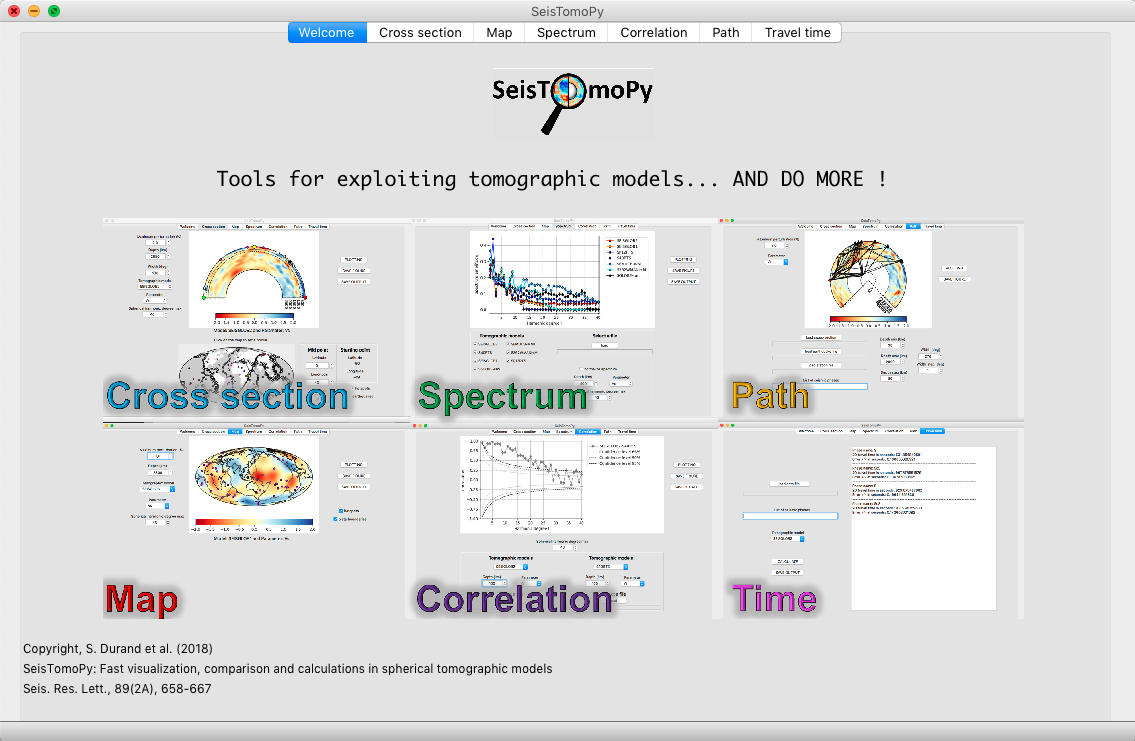
\includegraphics[scale=0.3]{SeisTomoPy_notebook/figures/welcome.png}
\caption{Welcoming screen of SeisTomoPy GUI interface.}
\label{welcome}
\end{center}
\end{figure}

    \subsection{Cross sections}\label{crosspy}

Go on the tab Cross section. A screen with a map at the bottom
and an empty space at the top appears. The parameters are already set to
default values so that clicking on the button PLOTTING (top
right button) computes a cross section.\\

Various options are available.  First, it is possible to choose the
location of the profile. To do so: 
\begin{itemize}
\item 1) Click on the map at the bottom
which will move the profile. This changes the mid-point of the
profile (yellow dot). One can also manually enter the values of the
latitude and longitude of the mid-point.
\item 2) Change the azimuth of the profile.
\end{itemize}
Other parameters that can be changed include: 
\begin{itemize}
\item 3) The width of the profile.
\item 4) The maximum depth down to which the cross section will be plotted.
\item 5) The tomographic model and parameter to be plotted.
\item 6) The spherical harmonic degree up to which the model will be plotted. It can be at most 60.
\item 7) The maximum values of the velocity perturbations used for the color bar.

\end{itemize}
All these actions are summarized on Figure 2.

\begin{figure}
\begin{center}
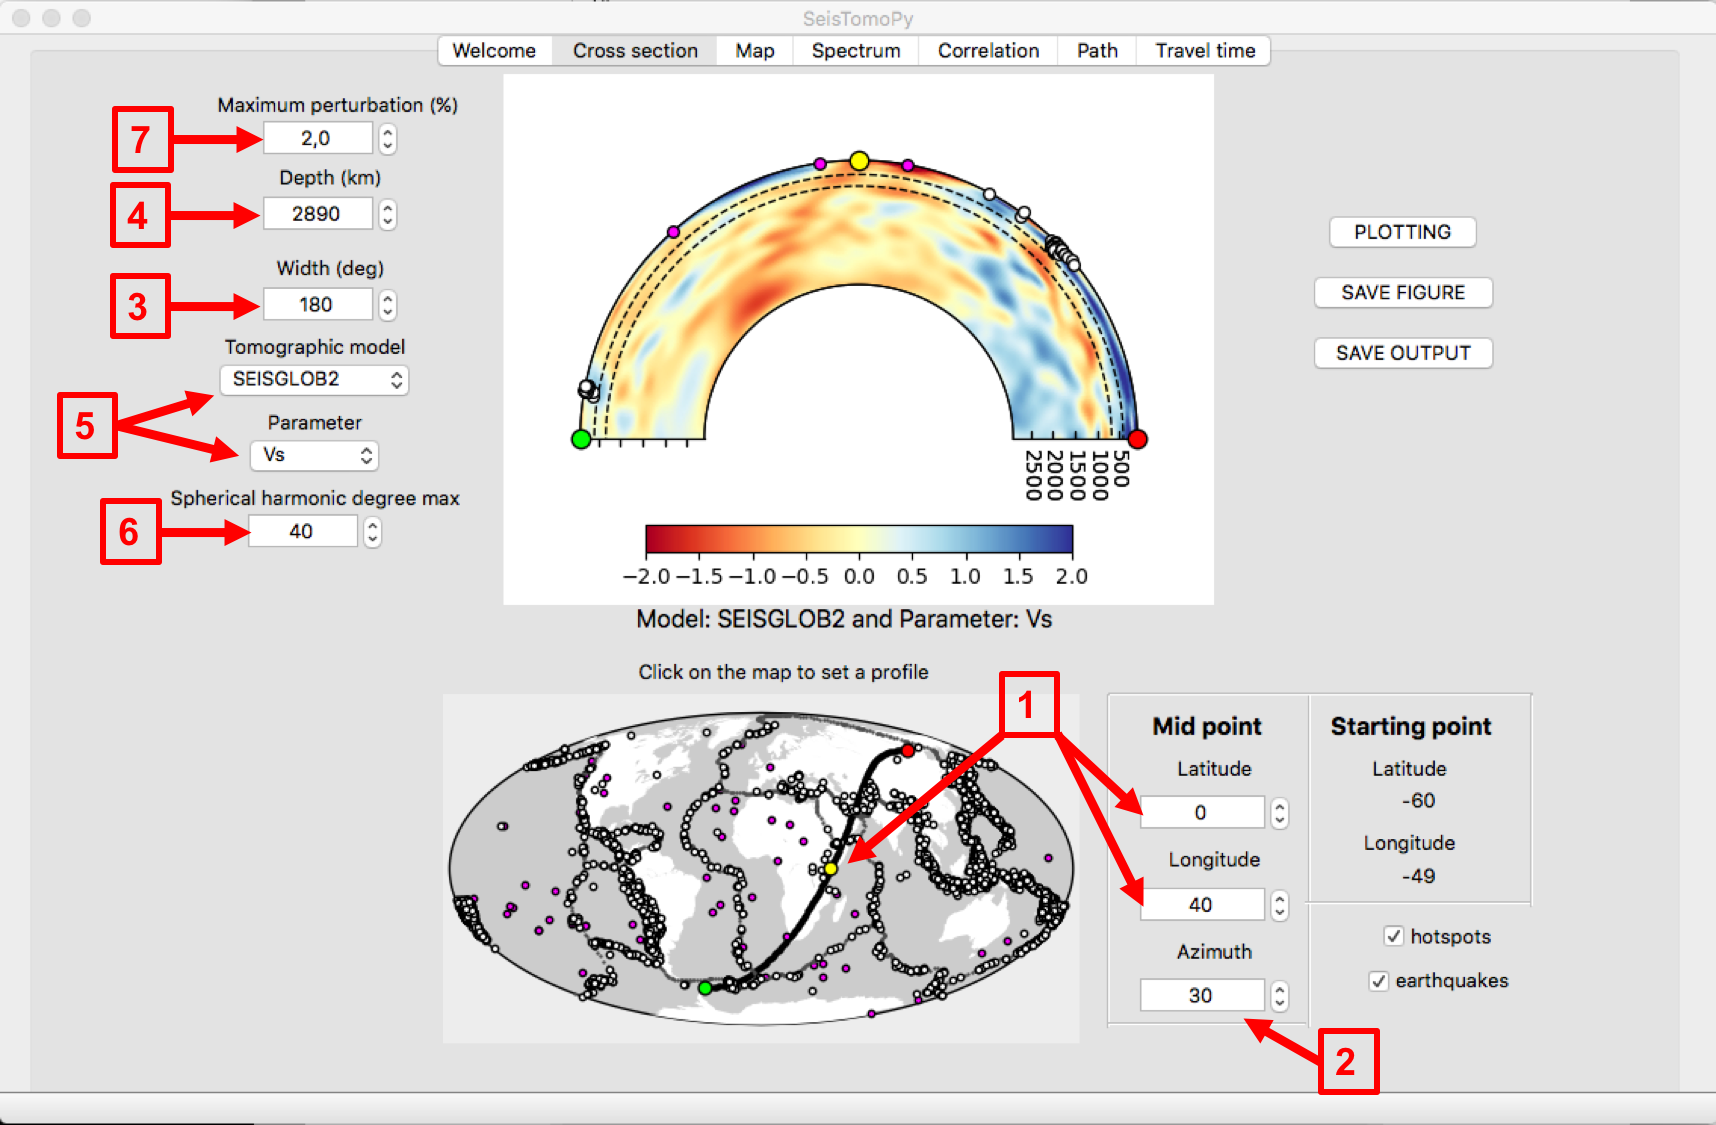
\includegraphics[scale=0.47]{SeisTomoPy_notebook/figures/crosspy.png}
\caption{Summary of the different options in Cross section.}
\label{crosspy}
\end{center}
\end{figure}

One can save the plots by clicking on SAVE FIGURE (top right button). This will produce two pdf files:
\begin{itemize}
\item
  \verb?map_MODEL_PARA_LAT_LON_AZI.pdf?
\item
 \verb?crossec_MODEL_PARA_LAT_LON_AZI.pdf?
\end{itemize}
MODEL, PARA, LAT, LON and AZI, respectively, correspond to the tomographic
model,  parameter, latitude and longitude of the mid-point and
 azimuth used for generating the profile.

Some useful output files can also be saved by clicking on SAVE OUTPUT. A
folder entitled \verb?output_crossection_LAT_LON_AZI? will appear at
the desired location. It contains 3 files:

\begin{itemize}
\item
  \verb?output_cross_MODEL.out?: file containing all the values to reproduce
  the cross section. There are 6 columns: latitude, longitude, radius
  (km), \(d\ln(V_p)\) (\%), \(d\ln(V_s)\) (\%), \(d\ln(\rho)\) (\%).
\item \verb?MODEL_input_AxiSEM.sph?: input file for running synthetic seismograms
  with AxiSEM.   \textcolor{red}{\textbf{It is important to note that these files give the velocity perturbations with respect to the reference model used in every tomographic inversion so that if the user provides  this file to AxiSEM, the good reference model file should also be provided. They are provided in }} \verb|Taup_models/AXISEM_REF|.
\item
  \verb?MODEL_PathPy.sph?: file that can be used in PathPy (see later).
\end{itemize}

\subsection{Maps}\label{mappy}

On the tab Maps, one finds a screen with an empty space  where the map will be plotted. The parameters are already set
to default values so that one can already click on the button PLOTTING
(top right button). After some seconds, the map will appear.\\

Parameters that can be changed include: 

\begin{itemize}
\item 1) The depth of the map.
\item 2) The tomographic model and parameter to be plotted.
 \item 3) The spherical harmonic degree up to which the model will be plotted.
    It can be at most 60.
\item 4) The central longitude.
\item 5) The maximum values of the velocity perturbations used for the
    color bar.
\end{itemize}
All these actions are summarized on Figure 3.

\begin{figure}
\begin{center}
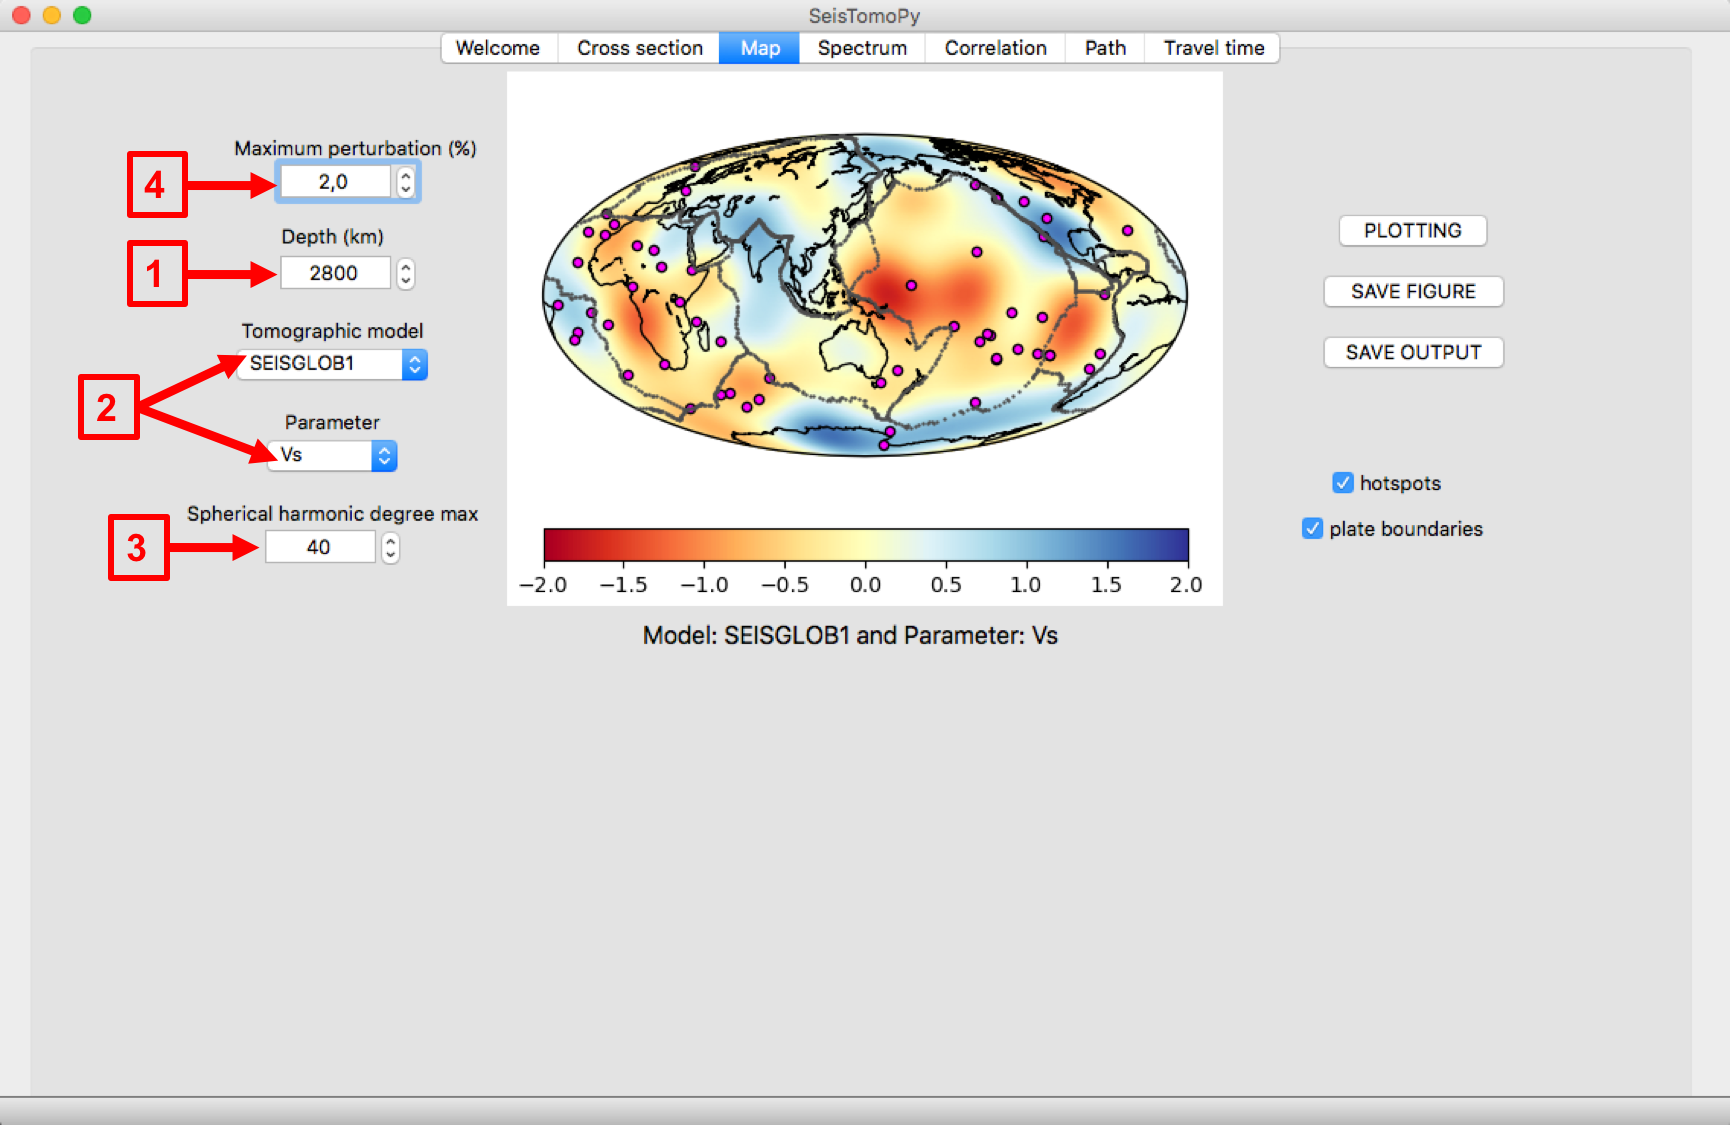
\includegraphics[scale=0.35]{SeisTomoPy_notebook/figures/mappy.png}
\caption{Summary of the different options in Map.}
\label{mappy}
\end{center}
\end{figure}

The plot can be saved by clicking on SAVE FIGURE (top right button).
This will produce one pdf file:

\begin{itemize}
\tightlist
\item
 \verb? map_MODEL_PARA_DEPTH.pdf?
\end{itemize}
MODEL, PARA and DEPTH, respectively, correspond  to the tomographic model,
 parameter and  depth used for generating the map.

Some useful output files can also be saved by clicking on SAVE OUTPUT. A
folder entitled \verb?output_map_DEPTH? will appear at the desired
location. It contains 4 files:

\begin{itemize}
\item
  3 files \verb?map_NEW_MODEL_PARA.out?: files containing all the values to
  reproduce the map. There are 3 columns: latitude, longitude,
  \(dln(PARA)\) (\%).
\item
  \verb?output_map_MODEL.out?: summary file with 5 columns: latitude,
  longitude, \(dln(V_p)\) (\%), \(dln(V_s)\) (\%), \(dln(\rho)\) (\%).
\end{itemize}

\subsection{Spectrum}\label{specpy}

On the tab Spectrum, the spectrum will be calculated. The parameters are already
set to default values so that clicking on the button
PLOTTING (top right button) produces a spectrum.\\


Parameters that can be changed include: 
\begin{itemize}
\item 1) The tomographic models to be
used.
\item 2) The depth at which the spectrum is being computed.
\item 3) The parameter.
\item 4) The spherical harmonic degree up to which the spectrum will be
    computed. It can be at most 60.
  \item 5)  It is also possible with this tool to compute the spectrum of any
    other model that the user wishes to use. Then the user must upload the
    file with the model at a given depth for a given parameter using the
    space entitle ``Select a file'' by clicking on the button ``load''.
    The file must have a specific format. Please refer to  section \ref{format} for details about these files.
\end{itemize}
All these actions are summarized on Figure 4.

\begin{figure}
\begin{center}
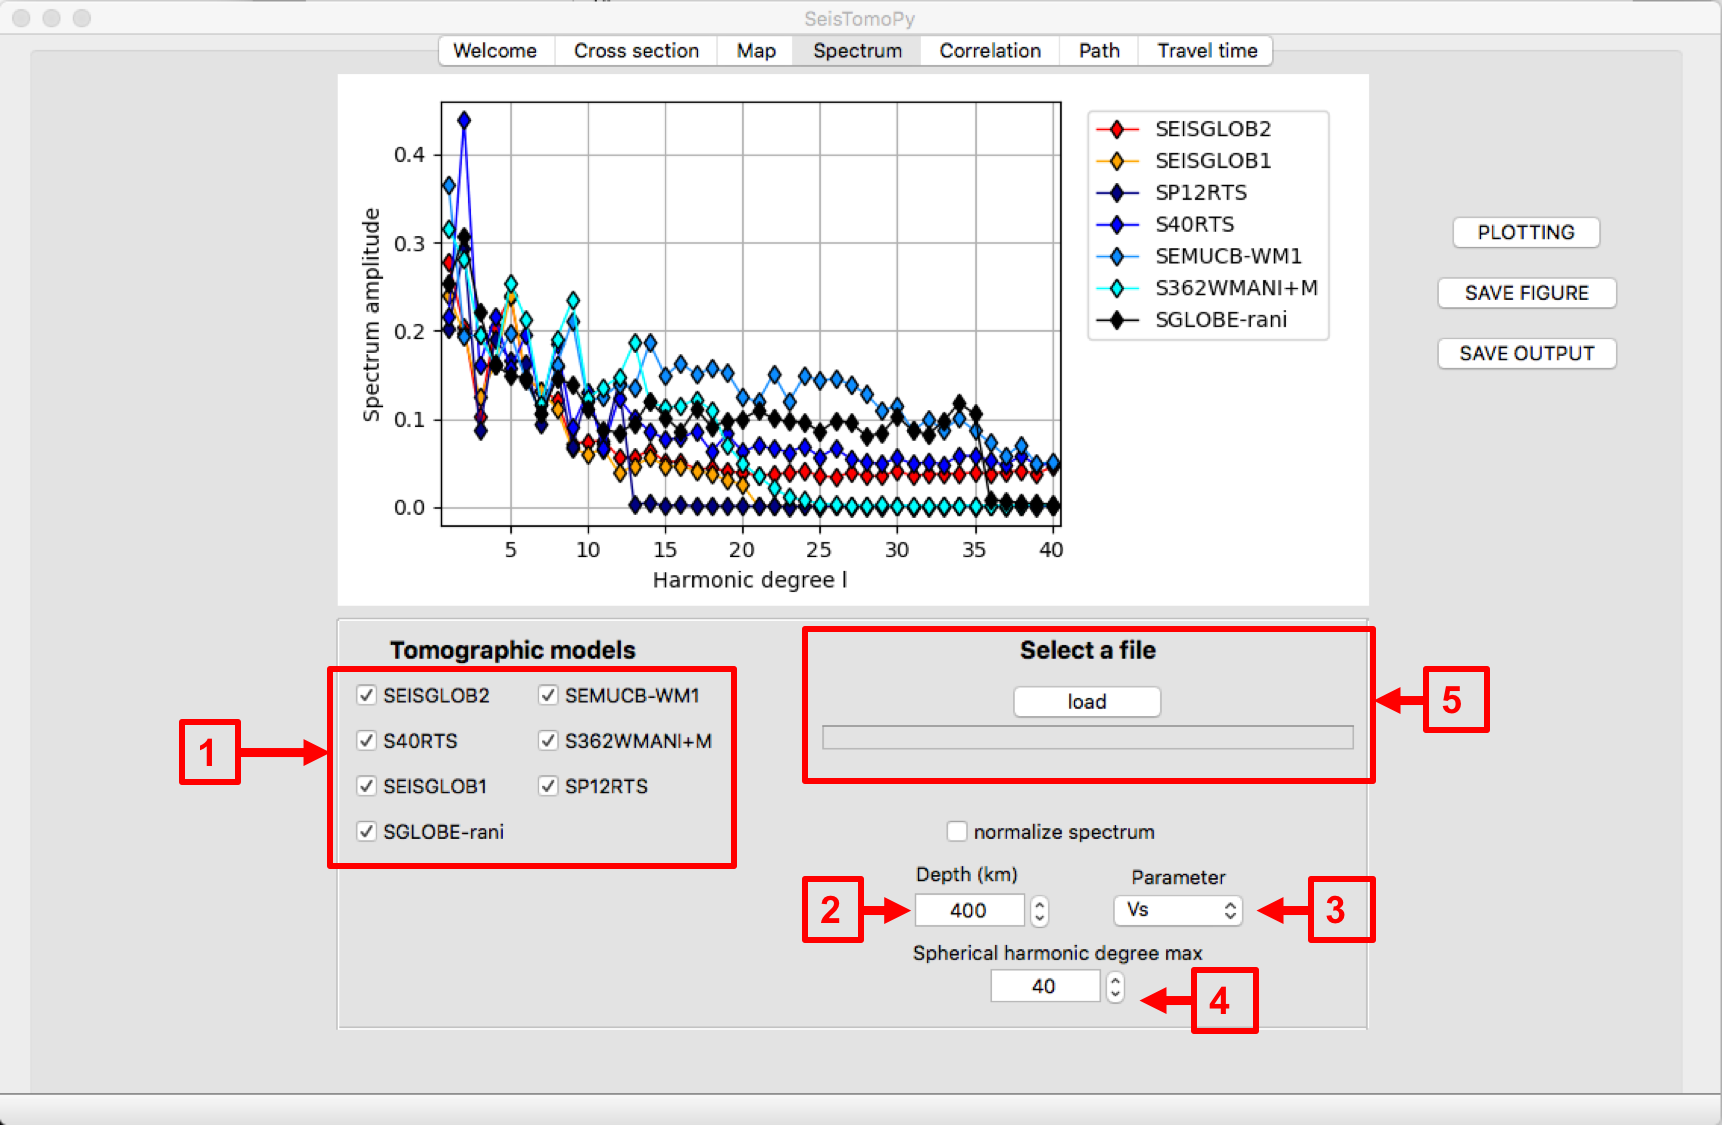
\includegraphics[scale=0.35]{SeisTomoPy_notebook/figures/specpy.png}
\caption{Summary of the different options in Spectrum.}
\label{specpy}
\end{center}
\end{figure}

One can save the plot by clicking on SAVE FIGURE (top right button).
This will produce one pdf file:

\begin{itemize}
\tightlist
\item
  \verb?spectre_DEPTH.pdf?
\end{itemize}
DEPTH corresponds to the depth at which the spectrum has been computed.

Some useful output files can be saved by clicking on SAVE OUTPUT. A
folder entitled \verb?output_spectre_DEPTH? will appear at the desired
location. It contains as many files as the number of tomographic models
used:

\begin{itemize}
\tightlist
\item
  \verb?spectre_MODEL_PARA_DEPTH.out?: file containing all the values of the
  spectrum. There are 2 columns: harmonic degree, spectrum.
\end{itemize}

\subsection{Correlations}\label{corrpy}

Tab Correlation calculates correlations between models.  The parameters are
already set to default values so that clicking on the
button PLOTTING (top right button) produces a correlation.\\

Parameters that can be changed include: 
\begin{itemize}
\item 1) The two tomographic models.
 \item 2)  The two depths.
  \item 3) The two parameters.
   \item 4)   The spherical harmonic degree up to which the spectrum will be
    computed. It can be at most 60.
 \item 5)    It is also possible with this tool to compute the correlation with
    any other model that the user wishes to use. The user must upload
    the file with the model at a given depth for a given parameter using
    the space entitled ``Select a file'' by clicking on the button
    ``load''.  The file must have a specific format. Please refer to  section \ref{format} for details about these files. If this option is to be
    used, then the tomographic model should be set to ``None''.
\end{itemize}
All these actions are summarized  on Figure 5.

\begin{figure}
\begin{center}
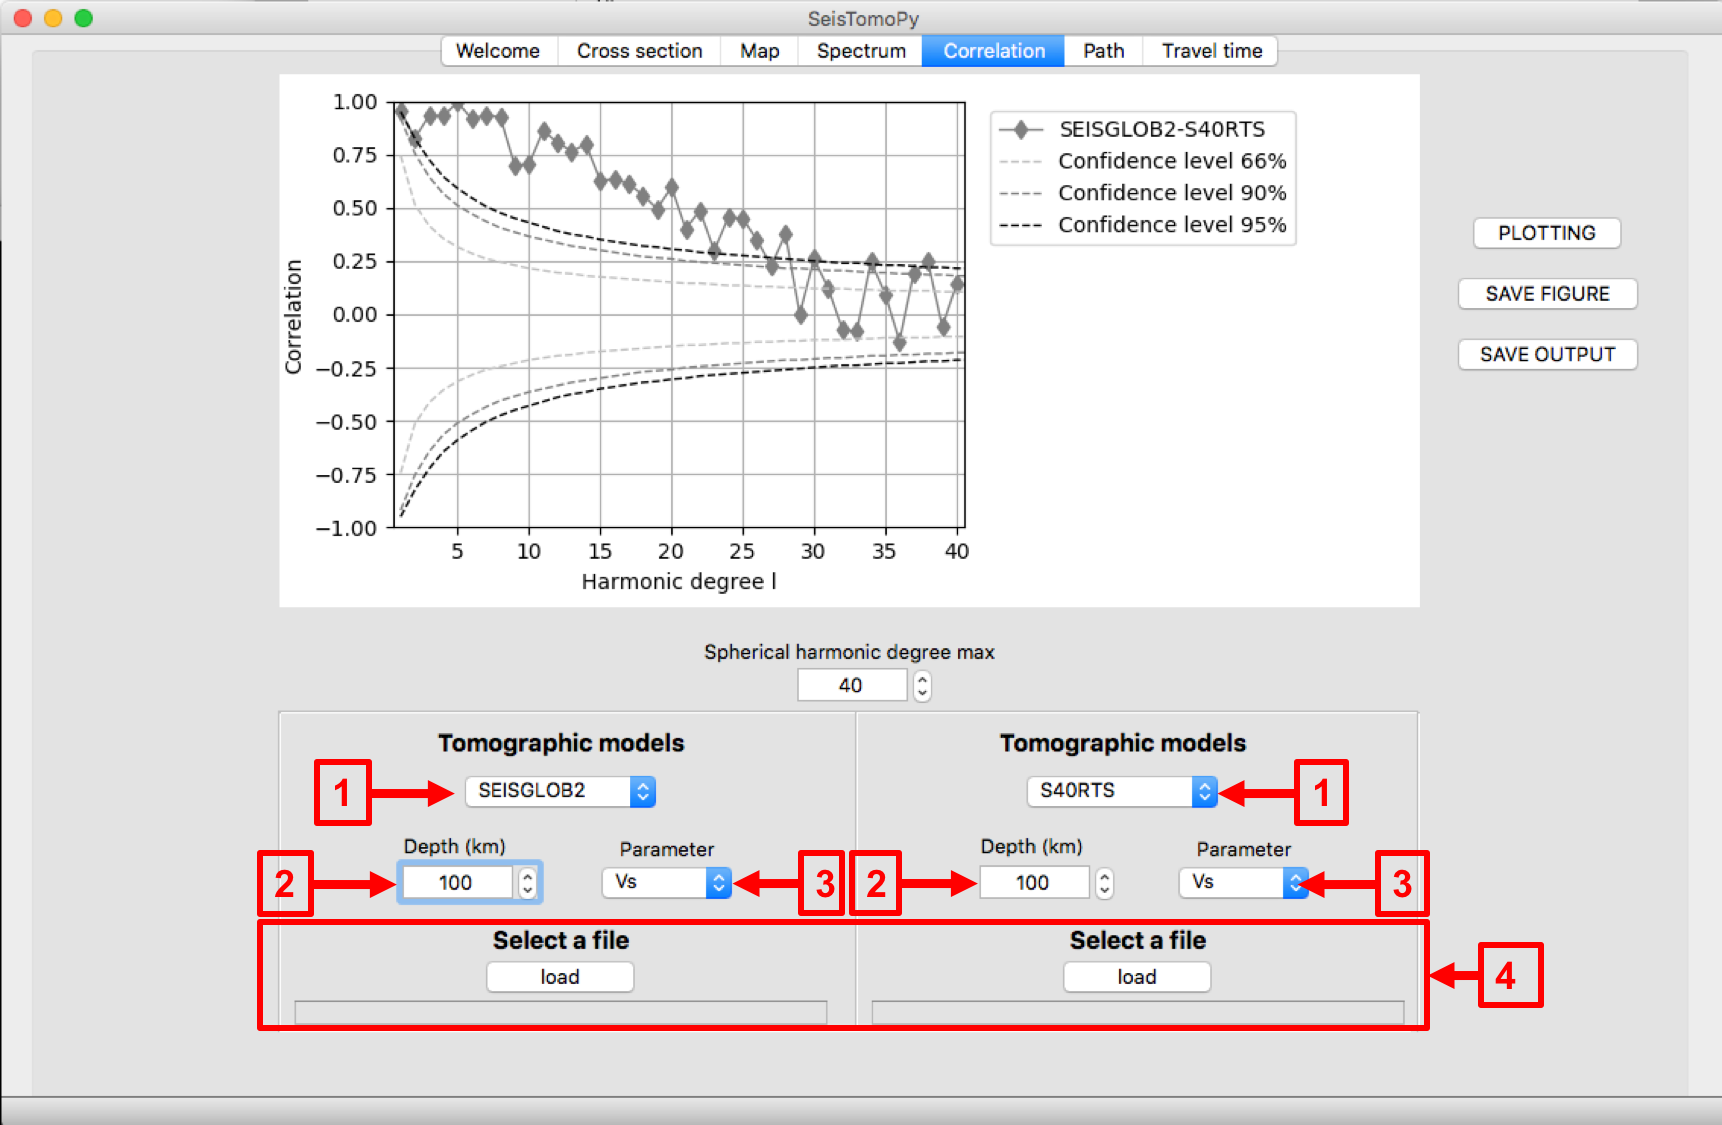
\includegraphics[scale=0.35]{SeisTomoPy_notebook/figures/corrpy.png}
\caption{Summary of the different options in Correlation.}
\label{corrpy}
\end{center}
\end{figure}

The plot can be saved by clicking on SAVE FIGURE (top right button). This will produce one pdf
file:
\begin{itemize}
\tightlist
\item
  \verb?correlation.pdf?
\end{itemize}

Some useful output files can also be saved by clicking on SAVE OUTPUT. A
folder entitled \verb?output\_corr? will appear at the desired location. It
contains 1 file:

\begin{itemize}
\tightlist
\item
  \verb?corr_MODEL1_MODEL2.out?: file containing all the values of the
  correlation. There are 2 columns: harmonic degree, correlation.
\end{itemize}

\subsection{Paths}\label{pathpy}

Tab Path allows to calculate paths and plot them on top of tomographic models. \\

The first thing to do with Path is
\begin{itemize}
 \item 1) to upload a cross section. This
can be achieved by clicking on ``load cross-section'' and first using
a file generated by the Cross section tool (\verb?MODEL_PathPy.sph?).
\item 2) Then in order to
properly read this file the user must give the starting and ending
depths in the file, as well as the depth step. The same for the width of the
cross section. It is then already possible to test wether the file is
properly read by clicking on PLOTTING. If yes, then a cross section 
is plotted (see Figure 6).

\begin{figure}
\begin{center}
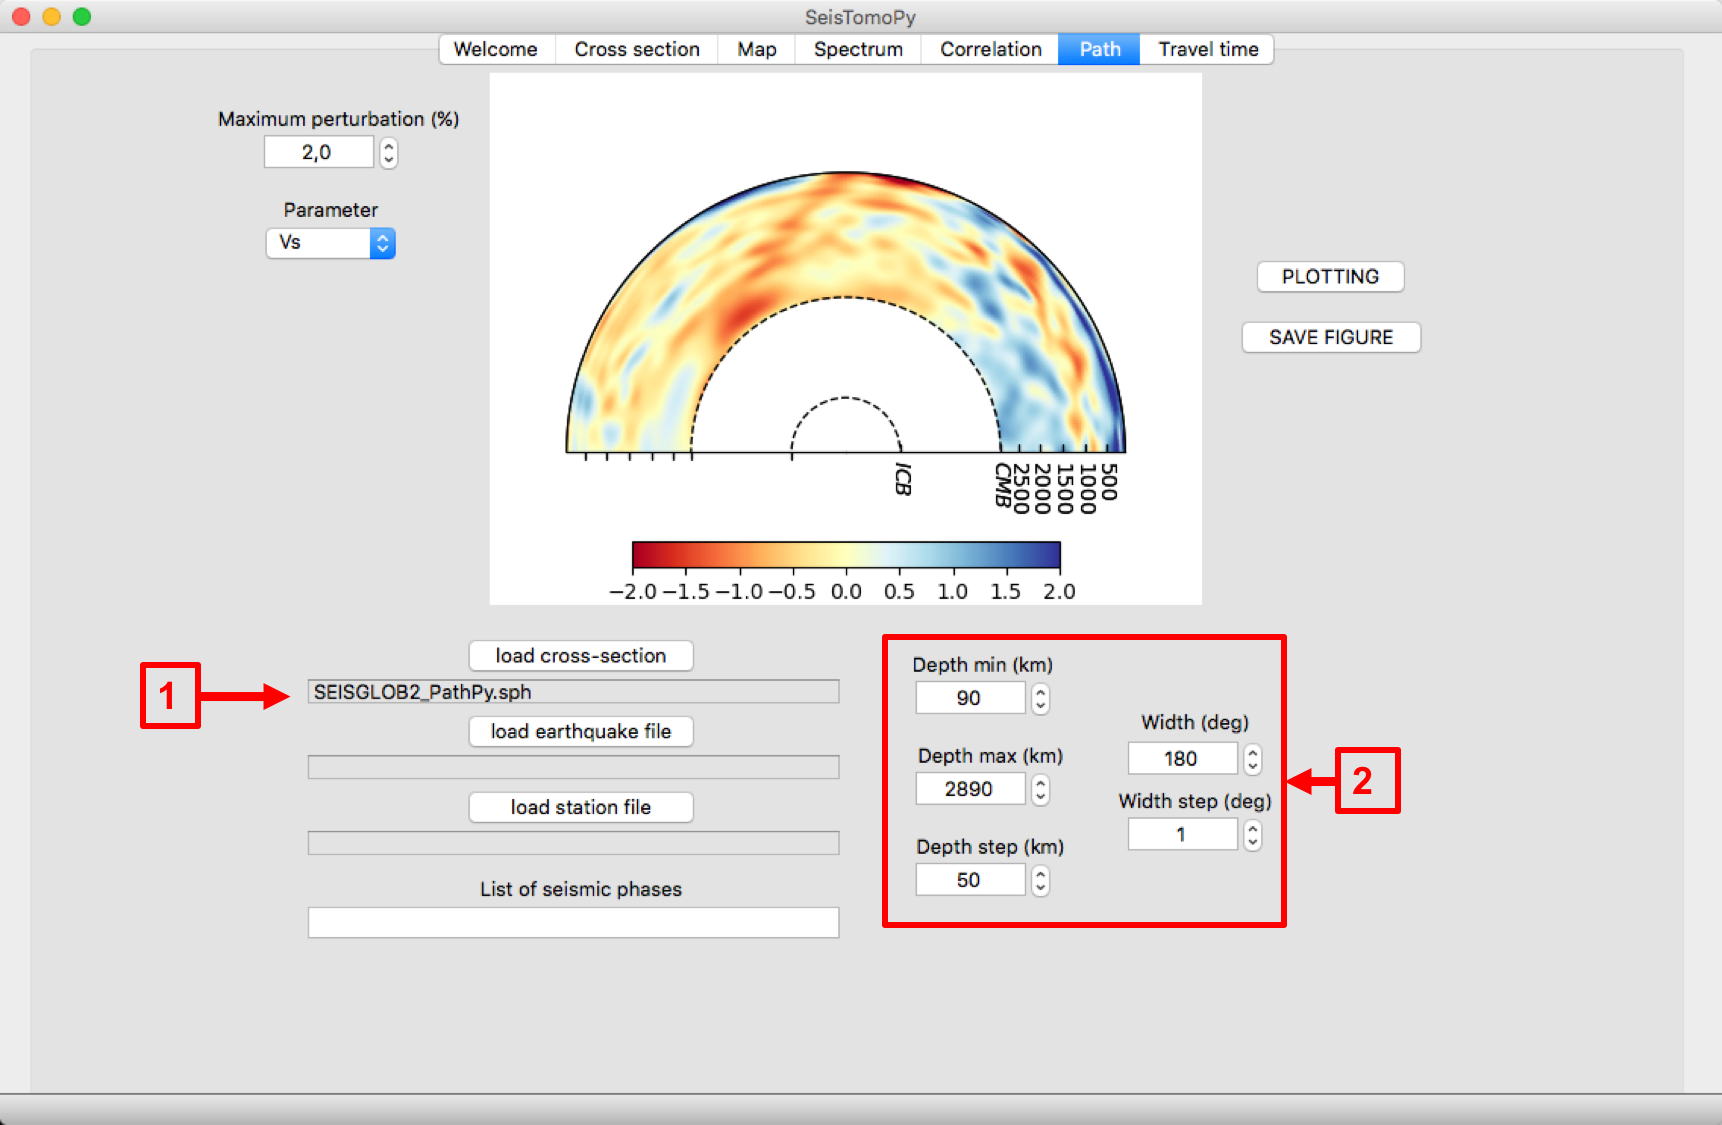
\includegraphics[scale=0.35]{SeisTomoPy_notebook/figures/pathpy1.png}
\caption{Summary of the different options in Path.}
\label{pathpy1}
\end{center}
\end{figure}

\item 3) Then one may want to plot  some seismic
wave paths on top of the cross section. To do so the user must choose a 1-D model used for the paths calculations. It can be chosen within the default ones or the user can also upload a 1-D model. Please refer to section \ref{format} for details about the model file.

\item 4) The user must also upload earthquake and station files. For the earthquake and station files,
they must contain two columns with the angle (in degrees) from the starting point of the profile and the depth
(in km) of the earthquakes and stations. For the example Figure 7 the following files \verb|event.xy|:

\begin{verbatim}
10 0
20 500
\end{verbatim}

\newpage
and \verb|station.xy|:

\begin{verbatim}
70 0
75 0
80 0
100 0
120 0
150 0
\end{verbatim}
have been used.

\item 5) Finally,  a list of seismic
phases should be provided. The list must contain the name of the seismic phases. If there is more than one they must be separated by a blank (for instance S ScS Sdiff ...). It is possible to run the calculations by clicking on PLOTTING, and
the cross section with the wave paths appears (see Figure 7).
\end{itemize}

\begin{figure}
\begin{center}
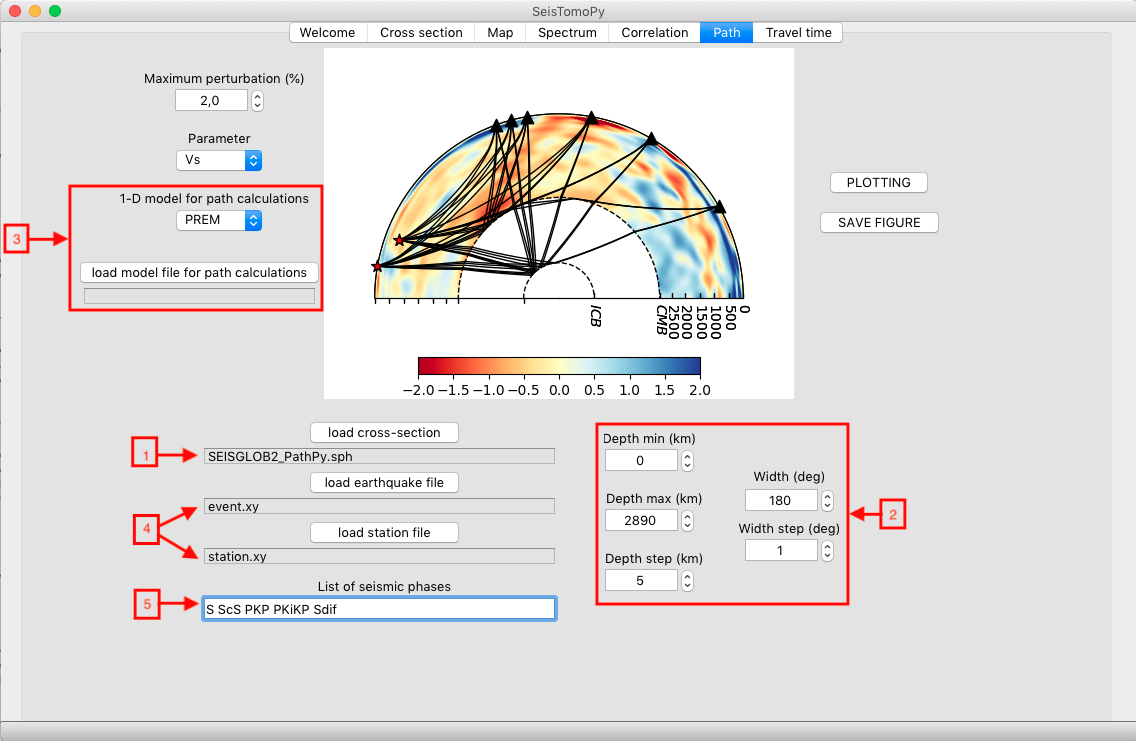
\includegraphics[scale=0.35]{SeisTomoPy_notebook/figures/pathpy2.png}
\caption{Summary of the different options in Path.}
\label{pathpy2}
\end{center}
\end{figure}

The plot can be saved by clicking on SAVE FIGURE and a \verb?path.pdf? file
will appear at the chosen location.

\subsection{Travel times}\label{timepy}

The last tool is Travel time. For this the user needs to
\begin{itemize}
\item 1) upload a file
with the earthquake and station locations. This file contains 5 columns
with event latitude, event longitude, event depth, station latitude and
station longitude.  For the example Figure 8 we used the file \verb|test.xy|:

\begin{verbatim}
0 0 200 0 30
0 0 200 0 50
\end{verbatim}

\item 2) Then the user must specify  the seismic waves to be
computed. If more than one is given the different phases must be separated by blanks (for instance S ScS Sdiff).
\item 3) Finally  a tomographic model must be chosen. The travel
time will be computed by clicking on CALCULATE. The summary of the
calculations will appear in the empty space on the right (see Figure 8).
\end{itemize}

The travel times can be saved by clicking on SAVE OUTPUT which will
create a folder travel\_times\_output.

\begin{figure}
\begin{center}
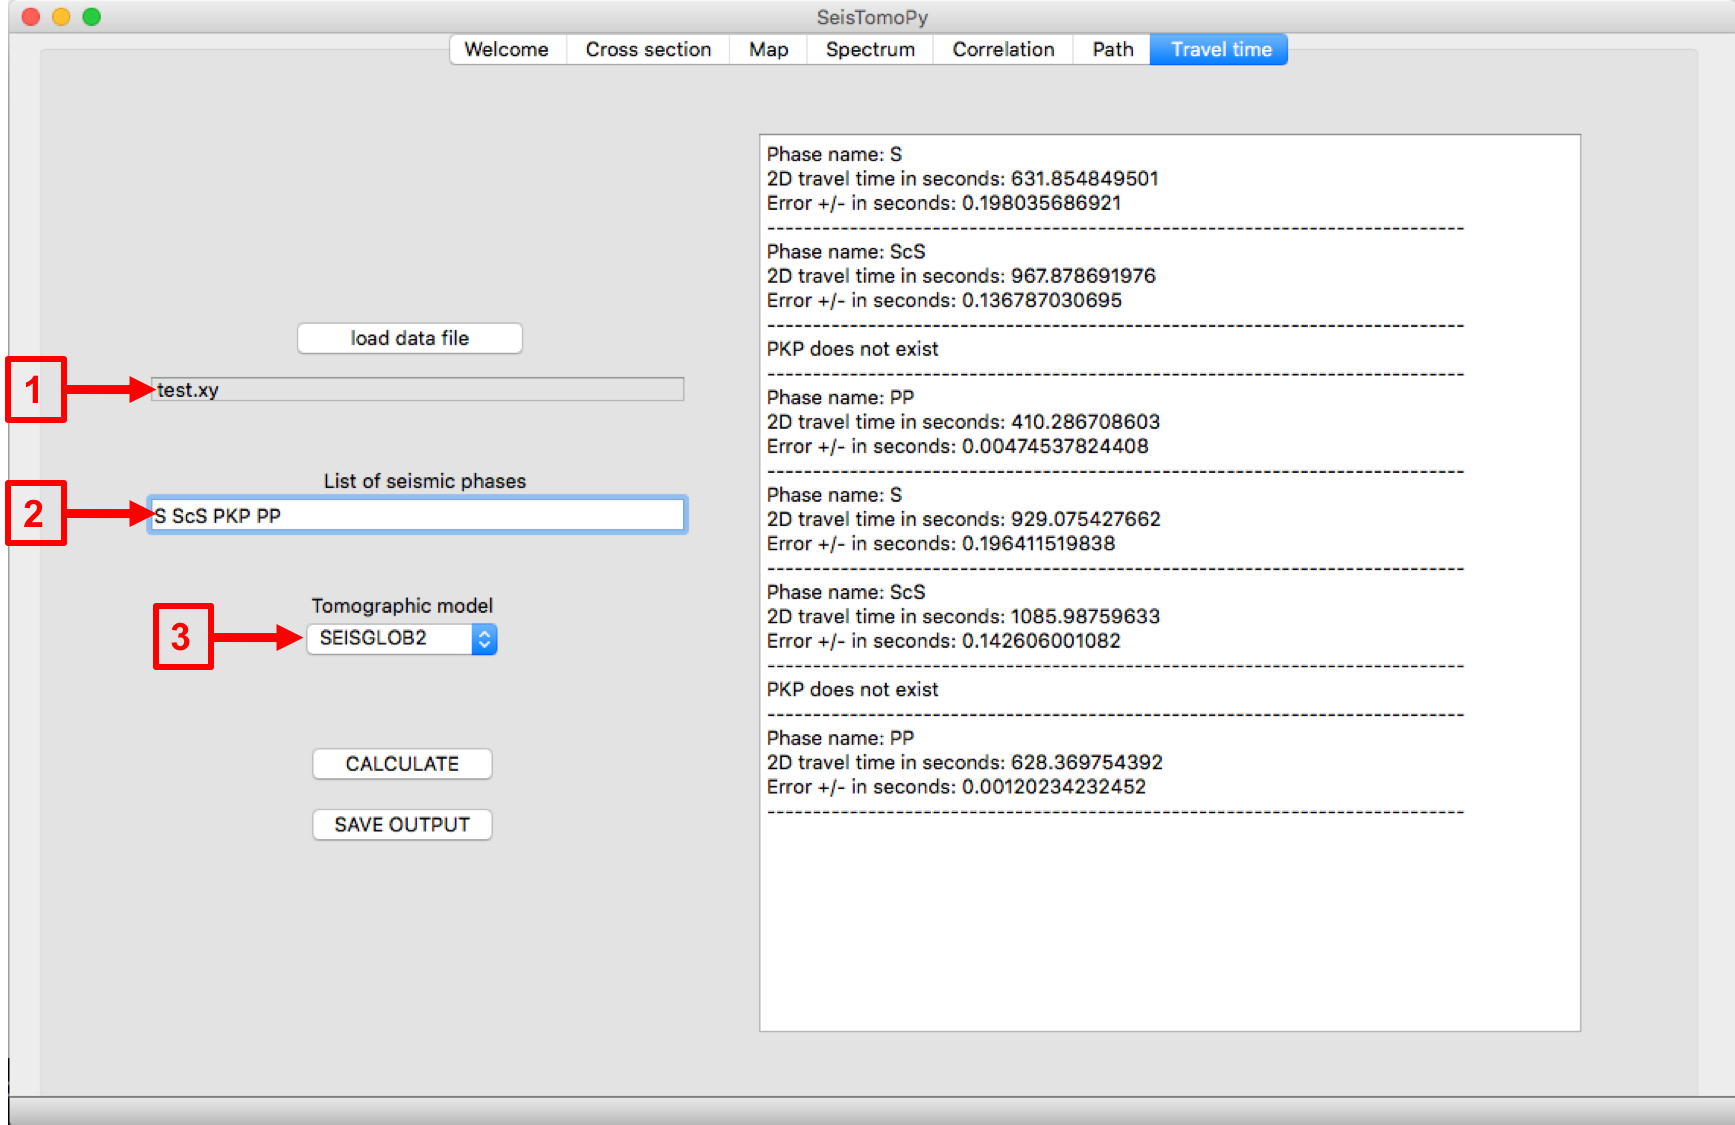
\includegraphics[scale=0.35]{SeisTomoPy_notebook/figures/timepy.png}
\caption{Summary of the different options in Travel time.}
\label{timrpy}
\end{center}
\end{figure}

\newpage

\section{Jupyter notebooks}\label{notebooks}

Jupyter notebooks have been developped as tutorial to facilitate the use of SeisTomoPy. You can access them by going to the folder 

\verb?$ cd SeisTomoPy/Documentation/SeisTomoPy_notebook?

Here you launch jupyter

\verb?$ jupyter notebook?

A web window should open and you will see two notebooks, one for learning how to use the SeisTomoPy classes and one for learning how to use the GUI interface.

\section{Model and parameter options}\label{models}

For using the tools, the tomographic models, parameters and 1-D models must be chosen. Here is the list of the acronyms to be used for the tomographic models:

   \begin{Verbatim}[commandchars=\\\{\},fontsize=\footnotesize]
\PY{l+s+s1}{\PYZdq{}}\PY{l+s+s1}{SEISGLOB2}\PY{l+s+s1}{\PYZdq{}}   
\PY{l+s+s1}{\PYZdq{}}\PY{l+s+s1}{S40RTS}\PY{l+s+s1}{\PYZdq{}}   
\PY{l+s+s1}{\PYZdq{}}\PY{l+s+s1}{SEMUCBWM1}\PY{l+s+s1}{\PYZdq{}}   
\PY{l+s+s1}{\PYZdq{}}\PY{l+s+s1}{S362WMANIM}\PY{l+s+s1}{\PYZdq{}}   
\PY{l+s+s1}{\PYZdq{}}\PY{l+s+s1}{SEISGLOB1}\PY{l+s+s1}{\PYZdq{}}   
\PY{l+s+s1}{\PYZdq{}}\PY{l+s+s1}{SP12RTS}\PY{l+s+s1}{\PYZdq{}}   
\PY{l+s+s1}{\PYZdq{}}\PY{l+s+s1}{SGLOBE}\PY{l+s+s1}{\PYZdq{}}   
\PY{l+s+s1}{\PYZdq{}}\PY{l+s+s1}{3D2016}\PY{l+s+s1}{\PYZdq{}}   
\PY{l+s+s1}{\PYZdq{}}\PY{l+s+s1}{MYMODEL}\PY{l+s+s1}{\PYZdq{}}   
  \end{Verbatim}

for the parameters

   \begin{Verbatim}[commandchars=\\\{\},fontsize=\footnotesize]
\PY{l+s+s1}{\PYZdq{}}\PY{l+s+s1}{VS}\PY{l+s+s1}{\PYZdq{}}   
\PY{l+s+s1}{\PYZdq{}}\PY{l+s+s1}{VP}\PY{l+s+s1}{\PYZdq{}}   
\PY{l+s+s1}{\PYZdq{}}\PY{l+s+s1}{RHO}\PY{l+s+s1}{\PYZdq{}}   
  \end{Verbatim}

and for the 1-D models

   \begin{Verbatim}[commandchars=\\\{\},fontsize=\footnotesize]
\PY{l+s+s1}{\PYZdq{}}\PY{l+s+s1}{prem}\PY{l+s+s1}{\PYZdq{}}   
\PY{l+s+s1}{\PYZdq{}}\PY{l+s+s1}{iasp91}\PY{l+s+s1}{\PYZdq{}}   
\PY{l+s+s1}{\PYZdq{}}\PY{l+s+s1}{ak135}\PY{l+s+s1}{\PYZdq{}}   
\PY{l+s+s1}{\PYZdq{}}\PY{l+s+s1}{pwdk}\PY{l+s+s1}{\PYZdq{}}   
  \end{Verbatim}


\section{Creating a new tomographic model file}\label{create}

It is possible to upload a new model in SeisTomoPy. For this the user has to generate the model file. To do so we provide a package. The user will find a directory \verb|Create_model_file| with a README file explaining the procedure. 

First the user must generate \verb|vs.DEPTH.xyz| files at every kilometer depth and store them in the directory \verb|Create_model_file/model| and then go to \verb|Create_model_file/src| and run 

  \verb?$ make clean?

  \verb?$ make all?

  \verb?$ ./main?

This will generate two model files   \verb?YOURMODEL_5km.sph? and   \verb?YOURMODEL_1km.sph? that should be copied in \verb|SeisTomoPy/fortran_files/models|. Then one can use all the tools of SeisTomoPy referring to the new model using 

   \begin{Verbatim}[commandchars=\\\{\},fontsize=\footnotesize]
\PY{l+s+s1}{\PYZdq{}}\PY{l+s+s1}{MYMODEL}\PY{l+s+s1}{\PYZdq{}}   
  \end{Verbatim}


\section{Changing plate boundary model and hot spots and earthquake catalogs}

 The plate boundaries of model NUVEL-1A \citep{demet90}, the hot spot locations \citep{muller93} and a catalog of earthquakes can be added. The catalog of earthquakes is not exhaustive, it has been built  with a minimum of earthquakes such that plate boundaries can be seen. We used events deeper than 100 km depth with magnitudes greater than 5.9 in the time range 1976-1998 and we added all events with magnitudes greater than 5.0 in the time range  2010-2011. Magnitudes were chosen to be larger than 5.0 to keep the dataset small. 

However, the user may want to use another plate boundary model, or hot spot and earthquake catalogs. To that aim it is possible to provide new files with the same format as those already provided and with the same name. 

\subsection{Plate boundary model}

The file must be named \verb|plate_boundaries.xy| and contains in the first column the longitude and in the second column the latitude of the plate boundaries. Every segment of boundary should be separated by NaN values as illustrated below.

\begin{verbatim}
...
    10.30000   -53.2000
     11.5000   -53.0000
     13.0000   -52.7000
     14.2000   -52.4000
     15.0000   -52.2000
     15.4000   -51.9000
NaN NaN
     15.3000   -51.9000
     16.1000   -51.9000
     16.4000   -52.1000
     17.3000   -52.4000
...
\end{verbatim}

\subsection{Hot spot catalog}

The file must be named \verb|points_chauds.xy| and contains in the first column the longitude of the hot spots and in the second column the latitude of the hot spots (see below). 

\begin{verbatim}
...
42.0000 12.0000 
-25.0000 -17.0000 
-14.3700 -7.9500 
-139.9699 -29.3722 
-28.0000 38.0000 
-113.0000 27.0000 
164.7017 -67.3982
...
\end{verbatim}

\subsection{Earthquake catalog}

The file must be named \verb|catalogue.xy| and contains in the first column the longitude of the event, in the second column the latitude of the event and in the third column the depth of the event (see below).

\begin{verbatim}
...
167.81 -15.97 174 
120.07 -7.37 623     
166.95 -14.91 103 
129.74 -6.90 186 
-177.61 -19.46 453        
70.64 36.33 196
-68.51 -20.54 134 
...
\end{verbatim}


\section{Input file formats for Spectrum, Correlations and Paths}\label{format}

It is possible to upload model files to be used in Spectrum, Correlation and Path. 

For Spectrum and Correlation the files have the same format and it is the same format as the files
    \verb?map_NEW_MODEL_PARA.out? obtained with Map tool, which have 3 columns:
    latitude (from -89 to 89 degrees, with a step of 1 degree),
    longitude (from 0 to 359 degrees, with a step of 1 degree) and
    parameter perturbations (\%). It must thus contain in total 64440 lines. Below is an extract given as example.

\begin{verbatim}
         -89           0  0.73245523974336291     
         -88           0  0.72104058555001316     
         -87           0  0.71041631025040164     
... 
          87         359  0.49352141683917167     
          88         359  0.51590110372203857     
          89         359  0.54502724312040074    
\end{verbatim}

For Path, the file must contain 5 columns: the radius, the distance in degrees from the starting point, $d\ln(V_p)$, $d\ln(V_s)$ and $d\ln(\rho)$ in \%. It is the same format as the files  \verb?MODEL_PathPy.sph? obtained with the Cross section tool. The user sets which parameter should be plotted in the input arguments of the function \verb?SeisTomoPy.path_plot_fromfile? or with the parameters to set on the GUI. Below is an example.

\begin{verbatim}
        3481           0   2.7162811E-002   4.9385717E-002   9.8771474E-003
        3531           0   3.3263616E-002   6.0478839E-002   1.2099678E-002
        3581           0   4.0070403E-002   7.2856784E-002   1.4571265E-002
...
        6131         180   1.2205796        2.2192353       0.4438470     
        6181         180   0.4952321        0.9005191       0.1801038     
        6231         180   0.7806580        1.4193792       0.2833848     
        6281         180   1.5027913        2.7322743       0.5464547     
\end{verbatim}

For path the user can also upload a 1-D model. This file must have the same format as \verb?*.nd? files used in TauP tool kit. It contains 6 columns: the depth (km), $V_p$ (km s$^{-1}$), $V_s$ (km s$^{-1}$),  $\rho$ (g cm$^{-3}$), $Q_\kappa$, $Q_\mu$. For major discontinuities (mantle, outer-core and inner-core) the discontinuity must be written. For any additional discontinuity tha user would like to add it should just be added where it is desired. Below is an example.

\begin{verbatim}
   0.00      5.80000   3.20000   2.60000    1456.0     600.0
   15.00     5.80000   3.20000   2.60000    1456.0     600.0
   15.00     6.80000   3.90000   2.90000    1350.0     600.0
   24.40     6.80000   3.90000   2.90000    1350.0     600.0
mantle
   24.40     8.11061   4.49094   3.38076    1446.0     600.0
   40.00     8.10119   4.48486   3.37906    1446.0     600.0
   60.00     8.08907   4.47715   3.37688    1447.0     600.0
...
 2271.00    13.13055   7.05525   5.25729     803.0     312.0
 2371.00    13.24532   7.09974   5.30724     807.0     312.0
 2471.00    13.36074   7.14423   5.35706     811.0     312.0
 2491.00    13.38410   7.15320   5.36700     812.0     312.0
 2491.00    13.91950   7.43930   5.58170     812.0     312.0
 2571.00    14.01650   7.47650   5.62310     815.0     312.0
 2671.00    14.13980   7.52340   5.67480     819.0     312.0
 2741.00    14.22760   7.55660   5.71110     822.0     312.0
 2771.00    14.23500   7.55640   5.72670     823.0     312.0
 2871.00    14.26020   7.55550   5.77870     826.0     312.0
 2891.00    14.26530   7.55520   5.78910     826.0     312.0
outer-core
 2891.00     8.06482   0.00000   9.90349   57822.0       0.0
 2971.00     8.19939   0.00000  10.02940   57822.0       0.0
 3071.00     8.36019   0.00000  10.18134   57822.0       0.0
 3171.00     8.51298   0.00000  10.32726   57822.0       0.0
...
 4971.00    10.24959   0.00000  12.06924   57822.0       0.0
 5071.00    10.30971   0.00000  12.12500   57822.0       0.0
 5149.50    10.35568   0.00000  12.16634   57822.0       0.0
inner-core
 5149.50    11.02827   3.50432  12.76360     445.0      85.0
 5171.00    11.03643   3.51002  12.77493     445.0      85.0
 5271.00    11.07249   3.53522  12.82501     443.0      85.0
...
 6271.00    11.26064   3.66670  13.08630     431.0      85.0
 6371.00    11.26220   3.66780  13.08848     431.0      85.0
\end{verbatim}


\section{Future developments }

Further functionalities will be added in the future:
%
\begin{itemize}
\item Displaying fully anisotropic tomographic models.
\item Displaying geodynamic models obtained from modeling codes such as Stag3D \citep{stag3D}, that can then be directly compared to tomographic models.
\end{itemize}

\section{Reference}

Please if you are using SeisTomoPy please refer to \\

\noindent S. Durand, R. Abreu, C. Thomas, 2018,\\
SeisTomoPy: Fast visualization, comparison and calculations in global tomographic models,\\
\srl \textbf{89}(2A), 658-667


\begin{thebibliography}{}

\bibitem[\textit{Bassin et al.,}(2000)]{bassin00}
Bassin, C., Laske, G., Masters, G., 2000,
The current limits of resolution for surface wave tomography in North America, 
\textit{EOS Trans AGU}, \textbf{81}, F897

\bibitem[\textit{Chang et al.}(2015)]{chang15}
Chang, S-J, Ferreira, A.M.G., Ritsema, J., van Heijst, H. J., Woodhouse, J.H., 2015, 
Joint inversion for global isotropic and radially anisotropic mantle structure including crustal thickness perturbations, 
\jgr \textbf{120}, 4,278-4,300. 

\bibitem[\textit{DeMets et al.}(1990)]{demet90}
DeMets, C., Gordon, R., Argus, D., 1990,
Current plate motions,
\gji \textbf{101}, 425-478.


\bibitem[\textit{Durand et al.}(2016)]{durand16}
Durand, S., Debayle, E., Ricard, Y., Lambotte, S., 2016, 
Seismic evidence for a change in the large scale tomographic pattern accross the D" layer, 
\grl \textbf{43}(15), 7,928-7,936. 

\bibitem[\textit{Durand et al.}(2017a)]{durand17a}
Durand, S., Debayle, E., Ricard, Y., Zaroli, C., Lambotte, S., 2017a, 
Confirmation of a change in the global shear velocity pattern at around 1,000 km depth, 
\gji \textit{revision}

\bibitem[\textit{Durand et al.}(2017b)]{durand17}
Durand, S., Abreu, R., Thomas, C., 2018, 
SeisTomoPy: Fast visualization, comparison and calculations in global tomographic models,
\srl \textbf{89}(2A), 658-667

\bibitem[\textit{French \& Romanowicz}(2014)]{french14}
French, S.W., Romanowicz, B., 2014, 
Whole-mantle radially anisotropic shear-velocity structure from spectral-element waveform tomography, 
\gji \textbf{199}, 1,303-1,327.

\bibitem[\textit{Koelemeijer et al.}(2016)]{koelemeijer16}
Koelemeijer, P. , Ritsema,J.,  Deuss, A., Van Heijst, H-J., 2016),
SP12RTS: a degree-12 model of shear- and compressional-wave velocity for Earth's mantle,
\gji \textbf{204}(2), 1,024-1,039.

\bibitem[\textit{Kustowski et al.}(2008)]{kustowski08}
Kustowski, B., Ekstrom, G.,  Dziewonski,  A. M., 2008,
Anisotropic shear-wave velocity structure of the Earth's mantle: A global model,
\jgr \textbf{113}B06306, doi:10.1029/2007JB005169.

\bibitem[\textit{Moulik \& Ekstr\"om}(2014)]{moulik13}
Moulik, P., Ekström, G., 2014, 
An anisotropic shear velocity model of the Earth's mantle using normal modes, body waves, surface waves and long-period waveforms, 
\gji \textbf{199}3, 1,713-1,738.

\bibitem[\textit{M\"uller et al.}(1993)]{muller93}
 M\"uller, R.D., Royer, J-Y., Lawver, L.A., 1993,
Revised plate motions relative to the hotspots from combined Atlantic and Indian ocean hotspot tracks,
\geo \textbf{21}, 275-278.

\bibitem[\textit{Nataf \& Ricard}(1993)]{nataf93}
Nataf, H., Ricard, Y.,1993, 
3SMAC: An a priori tomographic model of the upper mantle based on geophysical modeling,
\pepi, \textbf{95}, 101–122.

\bibitem[\textit{Ritsema et al.}(2011)]{ritsema11}
Ritsema, J., Deuss, A., van Heijst, H.J., Woodhouse, J.H., 2011,
S40RTS: a degree-40 shear-velocity model for the mantle from new Rayleigh wave dispersion, teleseismic traveltime and normal-mode splitting function measurements,
\gji \textbf{184}, 1,223-1,236.

\bibitem[\textit{Tackley \& Shunxing}(2002)]{stag3D}
Tackley, P., Shunxing, X., 2002,
The thermochemical structure and evolution of Earth{\textquoteright}s mantle: constraints and numerical models,
\textit{Philosophical Transactions of the Royal Society of London A: Mathematical, Physical and Engineering Sciences} \textbf{360}, 1,800 ,2,593-2,609.

\end{thebibliography}

    \end{document}
